\documentclass[twoside,11pt]{article}
\usepackage{epsfig}
\usepackage{rotating}

%%%\documentstyle[11pt,psfig]{article}
\pagestyle{myheadings}

% -----------------------------------------------------------------------------
% ? Document identification

\newcommand{\scusoft}          {{\sc Surf}}
\newcommand{\micron}           {$\mu$m}   

\newcommand{\stardoccategory}  {Starlink User Note}
\newcommand{\stardocinitials}  {SUN}
\newcommand{\stardocsource}    {sun\stardocnumber}
\newcommand{\stardocnumber}    {216.1}
\newcommand{\stardocauthors}   {T. Jenness, J.~F. Lightfoot\\
                                Joint Astronomy Centre, Hilo, Hawaii}
\newcommand{\stardocdate}      {30 June 1997}
\newcommand{\stardoctitle}     {SURF -- SCUBA User Reduction Facility}
\newcommand{\stardocversion}   {1.0-0}
\newcommand{\stardocmanual}    {User's manual}
\newcommand{\stardocabstract}  {%
\scusoft\ is a set of ADAM tasks necessary for reducing demodulated 
Submillimetre Common-User Bolometer Array (SCUBA) data obtained from
the James Clerk Maxwell Telescope. The tasks allows one to completely
re-reduce your SCUBA data.

This document describes how to reduce SCUBA data and includes detailed
descriptions of each task.
}
% ? End of document identification

% set up some common package names
\newcommand{\Kappa}{\xref{{\sc{Kappa}}}{sun95}{}}
\newcommand{\Figaro}{\xref{{\sc{Figaro}}}{sun86}{}}
\newcommand{\gaia}{\xref{{\sc{Gaia}}}{sun214}{}}
\newcommand{\convert}{\xref{{\sc{Convert}}}{sun55}{}}
\newcommand{\fluxes}{\xref{{\sc{Fluxes}}}{sun213}{}}
\newcommand{\Iras}{\xref{{\sc{Iras90}}}{sun163}{}}
\newcommand{\ndf}{\xref{NDF}{sun33}{}}
\newcommand{\agi}{\xref{AGI}{sun48}{}}

% Application tasks
\newcommand{\task}[1]{{\sf #1}}

% ADAM parameters
\newcommand{\param}[1]{{\tt #1}}

% Common tasks
\newcommand{\rebin}{\htmlref{\task{rebin}}{REBIN}}
\newcommand{\bolrebin}{\htmlref{\task{bolrebin}}{BOLREBIN}}
\newcommand{\intrebin}{\htmlref{\task{intrebin}}{INTREBIN}}
\newcommand{\chgqual}{\htmlref{\task{change\_quality}}{CHANGE_QUALITY}}
\newcommand{\chgflat}{\htmlref{\task{change\_flat}}{CHANGE_FLAT}}
\newcommand{\chgpnt}{\htmlref{\task{change\_pointing}}{CHANGE_POINTING}}
\newcommand{\chgdata}{\htmlref{\task{change\_data}}{CHANGE_DATA}}
\newcommand{\resw}{\htmlref{\task{reduce\_switch}}{REDUCE_SWITCH}}
\newcommand{\flatf}{\htmlref{\task{flatfield}}{FLATFIELD}}
\newcommand{\skydip}{\htmlref{\task{skydip}}{SKYDIP}}
\newcommand{\scuphot}{\htmlref{\task{scuphot}}{SCUPHOT}}
\newcommand{\ext}{\htmlref{\task{extinction}}{EXTINCTION}}
\newcommand{\scuquick}{\htmlref{\task{scuquick}}{SCUQUICK}}
\newcommand{\scuhelp}{\htmlref{\task{scuhelp}}{SCUHELP}}
\newcommand{\remsky}{\htmlref{\task{remsky}}{REMSKY}}
\newcommand{\scuover}{\htmlref{\task{scuover}}{SCUOVER}}
\newcommand{\extdata}{\htmlref{\task{extract\_data}}{EXTRACT_DATA}}
\newcommand{\sculog}{\htmlref{\task{sculog}}{SCULOG}}
\newcommand{\scucat}{\htmlref{\task{scucat}}{SCUCAT}}
\newcommand{\photsum}{\htmlref{\task{photsum}}{PHOTSUM}}
\newcommand{\mapsum}{\htmlref{\task{mapsum}}{MAPSUM}}
\newcommand{\pointsum}{\htmlref{\task{pointsum}}{POINTSUM}}
\newcommand{\qdraw}{\htmlref{\task{qdraw}}{QDRAW}}
\newcommand{\sigclip}{\htmlref{\task{sigclip}}{SIGCLIP}}
\newcommand{\restore}{\htmlref{\task{restore}}{RESTORE}}
\newcommand{\sdip}{\htmlref{\task{sdip}}{SDIP}}
\newcommand{\scupa}{\htmlref{\task{scupa}}{SCUPA}}
\newcommand{\obssum}{\htmlref{\task{obssum}}{OBSSUM}}

% Non surf tasks

\newcommand{\display}{\xref{\task{display}}{sun95}{DISPLAY}}
\newcommand{\linplot}{\xref{\task{linplot}}{sun95}{LINPLOT}}
\newcommand{\drawsig}{\xref{\task{drawsig}}{sun95}{DRAWSIG}}
\newcommand{\centroid}{\xref{\task{centroid}}{sun95}{CENTROID}}
\newcommand{\setaxis}{\xref{\task{setaxis}}{sun95}{SETAXIS}}
\newcommand{\kstest}{\xref{\task{kstest}}{sun95}{KSTEST}}
\newcommand{\stats}{\xref{\task{stats}}{sun95}{STATS}}
\newcommand{\thresh}{\xref{\task{thresh}}{sun95}{THRESH}}
\newcommand{\setbb}{\xref{\task{setbb}}{sun95}{SETBB}}
\newcommand{\fitslist}{\xref{\task{fitslist}}{sun95}{FITSLIST}}
\newcommand{\ndffits}{\xref{\task{ndf2fits}}{sun55}{NDF2FITS}}
\newcommand{\cadd}{\xref{\task{cadd}}{sun95}{CADD}}
\newcommand{\hdstrace}{\xref{\task{hdstrace}}{sun102}{}}
\newcommand{\psmerge}{\xref{\task{psmerge}}{sun164}{}}
\newcommand{\wdfits}{\xref{\task{wdfits}}{sun86}{WDFITS}}
\newcommand{\delobj}{\xref{\task{delobj}}{sun86}{DELOBJ}}
\newcommand{\setvar}{\xref{\task{setvar}}{sun95}{SETVAR}}
\newcommand{\ndfcopy}{\xref{\task{ndfcopy}}{sun95}{NDFCOPY}}
\newcommand{\gdset}{\xref{\task{gdset}}{sun95}{GDSET}}
\newcommand{\image}{\xref{\task{image}}{sun86}{IMAGE}}

%%% Some macros

% quick routine description. Now uses a description list

% This is the latex version

\newcommand{\quickdes}[3]{
\item \textbf{#1:} {\raggedright  #2 (page \pageref{#3})}}

% The HTML version is redefined later when the htmlonly environment
% is defined

% Environment for indenting and using a small font.
\newenvironment{myquote}{\begin{quote}\begin{small}}{\end{small}\end{quote}}

\newcommand{\text}[1]{{\small \tt #1}}

% -----------------------------------------------------------------------------

\newcommand{\stardocname}{\stardocinitials /\stardocnumber}
\markboth{\stardocname}{\stardocname}
\setlength{\textwidth}{160mm}
\setlength{\textheight}{230mm}
\setlength{\topmargin}{-2mm}
\setlength{\oddsidemargin}{0mm}
\setlength{\evensidemargin}{0mm}
\setlength{\parindent}{0mm}
\setlength{\parskip}{\medskipamount}
\setlength{\unitlength}{1mm}

% -----------------------------------------------------------------------------
%  Hypertext definitions.
%  ======================
%  These are used by the LaTeX2HTML translator in conjunction with star2html.

%  Comment.sty: version 2.0, 19 June 1992
%  Selectively in/exclude pieces of text.
%
%  Author
%    Victor Eijkhout                                      <eijkhout@cs.utk.edu>
%    Department of Computer Science
%    University Tennessee at Knoxville
%    104 Ayres Hall
%    Knoxville, TN 37996
%    USA

%  Do not remove the %\begin{rawtex} and %\end{rawtex} lines (used by 
%  star2html to signify raw TeX that latex2html cannot process).
%\begin{rawtex}
\makeatletter
\def\makeinnocent#1{\catcode`#1=12 }
\def\csarg#1#2{\expandafter#1\csname#2\endcsname}

\def\ThrowAwayComment#1{\begingroup
    \def\CurrentComment{#1}%
    \let\do\makeinnocent \dospecials
    \makeinnocent\^^L% and whatever other special cases
    \endlinechar`\^^M \catcode`\^^M=12 \xComment}
{\catcode`\^^M=12 \endlinechar=-1 %
 \gdef\xComment#1^^M{\def\test{#1}
      \csarg\ifx{PlainEnd\CurrentComment Test}\test
          \let\html@next\endgroup
      \else \csarg\ifx{LaLaEnd\CurrentComment Test}\test
            \edef\html@next{\endgroup\noexpand\end{\CurrentComment}}
      \else \let\html@next\xComment
      \fi \fi \html@next}
}
\makeatother

\def\includecomment
 #1{\expandafter\def\csname#1\endcsname{}%
    \expandafter\def\csname end#1\endcsname{}}
\def\excludecomment
 #1{\expandafter\def\csname#1\endcsname{\ThrowAwayComment{#1}}%
    {\escapechar=-1\relax
     \csarg\xdef{PlainEnd#1Test}{\string\\end#1}%
     \csarg\xdef{LaLaEnd#1Test}{\string\\end\string\{#1\string\}}%
    }}

%  Define environments that ignore their contents.
\excludecomment{comment}
\excludecomment{rawhtml}
\excludecomment{htmlonly}
%\end{rawtex}

%  Hypertext commands etc. This is a condensed version of the html.sty
%  file supplied with LaTeX2HTML by: Nikos Drakos <nikos@cbl.leeds.ac.uk> &
%  Jelle van Zeijl <jvzeijl@isou17.estec.esa.nl>. The LaTeX2HTML documentation
%  should be consulted about all commands (and the environments defined above)
%  except \xref and \xlabel which are Starlink specific.

\newcommand{\htmladdnormallinkfoot}[2]{#1\footnote{#2}}
\newcommand{\htmladdnormallink}[2]{#1}
\newcommand{\htmladdimg}[1]{}
\newenvironment{latexonly}{}{}
\newcommand{\hyperref}[4]{#2\ref{#4}#3}
\newcommand{\htmlref}[2]{#1}
\newcommand{\htmlimage}[1]{}
\newcommand{\htmladdtonavigation}[1]{}

%  Starlink cross-references and labels.
\newcommand{\xref}[3]{#1}
\newcommand{\xlabel}[1]{}

%  LaTeX2HTML symbol.
\newcommand{\latextohtml}{{\bf LaTeX}{2}{\tt{HTML}}}

%  Define command to re-centre underscore for Latex and leave as normal
%  for HTML (severe problems with \_ in tabbing environments and \_\_
%  generally otherwise).
\newcommand{\latex}[1]{#1}
\newcommand{\setunderscore}{\renewcommand{\_}{{\tt\symbol{95}}}}
\latex{\setunderscore}

%  Redefine the \tableofcontents command. This procrastination is necessary 
%  to stop the automatic creation of a second table of contents page
%  by latex2html.
\newcommand{\latexonlytoc}[0]{\tableofcontents}

% -----------------------------------------------------------------------------
%  Debugging.
%  =========
%  Remove % on the following to debug links in the HTML version using Latex.

% \newcommand{\hotlink}[2]{\fbox{\begin{tabular}[t]{@{}c@{}}#1\\\hline{\footnotesize #2}\end{tabular}}}
% \renewcommand{\htmladdnormallinkfoot}[2]{\hotlink{#1}{#2}}
% \renewcommand{\htmladdnormallink}[2]{\hotlink{#1}{#2}}
% \renewcommand{\hyperref}[4]{\hotlink{#1}{\S\ref{#4}}}
% \renewcommand{\htmlref}[2]{\hotlink{#1}{\S\ref{#2}}}
% \renewcommand{\xref}[3]{\hotlink{#1}{#2 -- #3}}
% -----------------------------------------------------------------------------
% ? Document specific \newcommand or \newenvironment commands.
% ? End of document specific commands
% -----------------------------------------------------------------------------
%  Title Page.
%  ===========
\renewcommand{\thepage}{\roman{page}}

% quickdes For HTML
\begin{htmlonly}
\renewcommand{\quickdes}[3]{ \item[\htmlref{#1}{#1}:] {#2}}
\end{htmlonly}



%%%% START 

\begin{document}
\thispagestyle{empty}

%  Latex document header.
%  ======================
\begin{latexonly}
   CCLRC / {\sc Rutherford Appleton Laboratory} \hfill {\bf \stardocname}\\
   {\large Particle Physics \& Astronomy Research Council}\\
   {\large Starlink Project\\}
   {\large \stardoccategory\ \stardocnumber}
   \begin{flushright}
   \stardocauthors\\
   \stardocdate
   \end{flushright}
   \vspace{-4mm}
   \rule{\textwidth}{0.5mm}
   \vspace{5mm}
   \begin{center}
   
\epsfig{file=sun216_logo.eps,width=2.0in}

   {\Huge\bf  \stardoctitle \\ [2.5ex]}
   {\LARGE\bf \stardocversion \\ [4ex]}
   {\Huge\bf  \stardocmanual}
   \end{center}
   \vspace{5mm}

% ? Heading for abstract if used.
   \vspace{10mm}
   \begin{center}
      {\Large\bf Abstract}
   \end{center}
% ? End of heading for abstract.
\end{latexonly}

%  HTML documentation header.
%  ==========================
\begin{htmlonly}
   \xlabel{}
   \begin{rawhtml} <H1> \end{rawhtml}
      \stardoctitle\\
      \stardocversion\\
      \stardocmanual
   \begin{rawhtml} </H1> \end{rawhtml}

% ? Add picture here if required.
   
\epsfig{width=2.0in,file=sun216_logo.eps}

% ? End of picture

   \begin{rawhtml} <P> <I> \end{rawhtml}
   \stardoccategory \stardocnumber \\
   \stardocauthors \\
   \stardocdate
   \begin{rawhtml} </I> </P> <H3> \end{rawhtml}
      \htmladdnormallink{CCLRC}{http://www.cclrc.ac.uk} /
      \htmladdnormallink{Rutherford Appleton Laboratory}
                        {http://www.cclrc.ac.uk/ral} \\
      \htmladdnormallink{Particle Physics \& Astronomy Research Council}
                        {http://www.pparc.ac.uk} \\
   \begin{rawhtml} </H3> <H2> \end{rawhtml}
      \htmladdnormallink{Starlink Project}{http://star-www.rl.ac.uk/}
   \begin{rawhtml} </H2> \end{rawhtml}
   \htmladdnormallink{\htmladdimg{source.gif} Retrieve hardcopy}
      {http://star-www.rl.ac.uk/cgi-bin/hcserver?\stardocsource}\\

%  HTML document table of contents. 
%  ================================
%  Add table of contents header and a navigation button to return to this 
%  point in the document (this should always go before the abstract \section). 
  \label{stardoccontents}
  \begin{rawhtml} 
    <HR>
    <H2>Contents</H2>
  \end{rawhtml}
  \renewcommand{\latexonlytoc}[0]{}
  \htmladdtonavigation{\htmlref{\htmladdimg{contents_motif.gif}}
        {stardoccontents}}

% ? New section for abstract if used.
  \section{\xlabel{abstract}Abstract}
% ? End of new section for abstract
\end{htmlonly}

% -----------------------------------------------------------------------------
% ? Document Abstract. (if used)
%  ==================
\stardocabstract
% ? End of document abstract
% -----------------------------------------------------------------------------
% ? Latex document Table of Contents (if used).
%  ===========================================
 \newpage
 \begin{latexonly}
   \setlength{\parskip}{0mm}
   \latexonlytoc
   \setlength{\parskip}{\medskipamount}
   \markboth{\stardocname}{\stardocname}
 \end{latexonly}
% ? End of Latex document table of contents
% -----------------------------------------------------------------------------
\cleardoublepage
\renewcommand{\thepage}{\arabic{page}}
\setcounter{page}{1}

% +
%  Name:
%     SST.TEX
 
%  Purpose:
%     Define LaTeX commands for laying out Starlink routine descriptions.
 
%  Language:
%     LaTeX
 
%  Type of Module:
%     LaTeX data file.
 
%  Description:
%     This file defines LaTeX commands which allow routine documentation
%     produced by the SST application PROLAT to be processed by LaTeX and
%     by LaTeX2html. The contents of this file should be included in the
%     source prior to any statements that make of the sst commnds.
 
%  Notes:
%     The commands defined in the style file html.sty provided with LaTeX2html
%     are used. These should either be made available by using the appropriate
%     sun.tex (with hypertext extensions) or by putting the file html.sty
%     on your TEXINPUTS path (and including the name as part of the
%     documentstyle declaration).
 
%  Authors:
%     RFWS: R.F. Warren-Smith (STARLINK)
%     PDRAPER: P.W. Draper (Starlink - Durham University)
 
%  History:
%     10-SEP-1990 (RFWS):
%        Original version.
%     10-SEP-1990 (RFWS):
%        Added the implementation status section.
%     12-SEP-1990 (RFWS):
%        Added support for the usage section and adjusted various spacings.
%     8-DEC-1994 (PDRAPER):
%        Added support for simplified formatting using LaTeX2html.
%     {enter_further_changes_here}
 
%  Bugs:
%     {note_any_bugs_here}
 
% -
 
%  Define length variables.
\newlength{\sstbannerlength}
\newlength{\sstcaptionlength}
\newlength{\sstexampleslength}
\newlength{\sstexampleswidth}
 
%  Define a \tt font of the required size.
\newfont{\ssttt}{cmtt10 scaled 1095}
 
%  Define a command to produce a routine header, including its name,
%  a purpose description and the rest of the routine's documentation.
\newcommand{\sstroutine}[3]{
   \goodbreak
   \rule{\textwidth}{0.5mm}
   \vspace{-7ex}
   \newline
   \settowidth{\sstbannerlength}{{\Large {\bf #1}}}
   \setlength{\sstcaptionlength}{\textwidth}
   \setlength{\sstexampleslength}{\textwidth}
   \addtolength{\sstbannerlength}{0.5em}
   \addtolength{\sstcaptionlength}{-2.0\sstbannerlength}
   \addtolength{\sstcaptionlength}{-5.0pt}
   \settowidth{\sstexampleswidth}{{\bf Examples:}}
   \addtolength{\sstexampleslength}{-\sstexampleswidth}
   \parbox[t]{\sstbannerlength}{\flushleft{\Large {\bf #1}}}
   \parbox[t]{\sstcaptionlength}{\center{\Large #2}}
   \parbox[t]{\sstbannerlength}{\flushright{\Large {\bf #1}}}
   \begin{description}
      #3
   \end{description}
}
 
%  Format the description section.
\newcommand{\sstdescription}[1]{\item[Description:] #1}
 
%  Format the usage section.
\newcommand{\sstusage}[1]{\item[Usage:] \mbox{} \\[1.3ex] {\ssttt #1}}
 
 
%  Format the invocation section.
\newcommand{\sstinvocation}[1]{\item[Invocation:]\hspace{0.4em}{\tt #1}}
 
%  Format the arguments section.
\newcommand{\sstarguments}[1]{
   \item[Arguments:] \mbox{} \\
   \vspace{-3.5ex}
   \begin{description}
      #1
   \end{description}
}
 
%  Format the returned value section (for a function).
\newcommand{\sstreturnedvalue}[1]{
   \item[Returned Value:] \mbox{} \\
   \vspace{-3.5ex}
   \begin{description}
      #1
   \end{description}
}
 
%  Format the parameters section (for an application).
\newcommand{\sstparameters}[1]{
   \item[Parameters:] \mbox{} \\
   \vspace{-3.5ex}
   \begin{description}
      #1
   \end{description}
}
 
%  Format the examples section.
\newcommand{\sstexamples}[1]{
   \item[Examples:] \mbox{} \\
   \vspace{-3.5ex}
   \begin{description}
      #1
   \end{description}
}
 
%  Define the format of a subsection in a normal section.
\newcommand{\sstsubsection}[1]{ \item[{#1}] \mbox{} \\}
 
%  Define the format of a subsection in the examples section.
\newcommand{\sstexamplesubsection}[2]{\sloppy
\item[\parbox{\sstexampleslength}{\ssttt #1}] \mbox{} \\ #2 }
 
%  Format the notes section.
\newcommand{\sstnotes}[1]{\item[Notes:] \mbox{} \\[1.3ex] #1}
 
%  Provide a general-purpose format for additional (DIY) sections.
\newcommand{\sstdiytopic}[2]{\item[{\hspace{-0.35em}#1\hspace{-0.35em}:}] \mbox{} \\[1.3ex] #2}
 
%  Format the implementation status section.
\newcommand{\sstimplementationstatus}[1]{
   \item[{Implementation Status:}] \mbox{} \\[1.3ex] #1}
 
%  Format the bugs section.
\newcommand{\sstbugs}[1]{\item[Bugs:] #1}
 
%  Format a list of items while in paragraph mode.
\newcommand{\sstitemlist}[1]{
  \mbox{} \\
  \vspace{-3.5ex}
  \begin{itemize}
     #1
  \end{itemize}
}
 
%  Define the format of an item.
\newcommand{\sstitem}{\item}
 
%  Now define html equivalents of those already set. These are used by
%  latex2html and are defined in the html.sty files.
\begin{htmlonly}
 
%  Re-define \ssttt.
   \newcommand{\ssttt}{\tt}
 
%  sstroutine.
   \renewcommand{\sstroutine}[3]{
      \subsection{#1\xlabel{#1}-\label{#1}#2}
      \begin{description}
         #3
      \end{description}
   }
 
%  sstdescription
   \renewcommand{\sstdescription}[1]{\item[Description:]
      \begin{description}
         #1
      \end{description}
   }
 
%  sstusage
   \renewcommand{\sstusage}[1]{\item[Usage:]
      \begin{description}
         {\ssttt #1}
      \end{description}
   }
 
%  sstinvocation
   \renewcommand{\sstinvocation}[1]{\item[Invocation:]
      \begin{description}
         {\ssttt #1}
      \end{description}
   }
 
%  sstarguments
   \renewcommand{\sstarguments}[1]{
      \item[Arguments:]
      \begin{description}
         #1
      \end{description}
   }
 
%  sstreturnedvalue
   \renewcommand{\sstreturnedvalue}[1]{
      \item[Returned Value:]
      \begin{description}
         #1
      \end{description}
   }
 
%  sstparameters
   \renewcommand{\sstparameters}[1]{
      \item[Parameters:]
      \begin{description}
         #1
      \end{description}
   }
 
%  sstexamples
   \renewcommand{\sstexamples}[1]{
      \item[Examples:]
      \begin{description}
         #1
      \end{description}
   }
 
%  sstsubsection
   \renewcommand{\sstsubsection}[1]{\item[{#1}]}
 
%  sstexamplesubsection
   \renewcommand{\sstexamplesubsection}[2]{\item[{\ssttt #1}] \\ #2}
 
%  sstnotes
   \renewcommand{\sstnotes}[1]{\item[Notes:]
      \begin{description}
         #1
      \end{description}
   }
 
%  sstdiytopic
   \renewcommand{\sstdiytopic}[2]{\item[{#1}]
      \begin{description}
         #2
      \end{description}
   }
 
%  sstimplementationstatus
   \renewcommand{\sstimplementationstatus}[1]{\item[Implementation Status:]
      \begin{description}
         #1
      \end{description}
   }
 
%  sstitemlist
   \newcommand{\sstitemlist}[1]{
      \begin{itemize}
         #1
      \end{itemize}
   }
\end{htmlonly}
 
%  End of "sst.tex" layout definitions.
% .
% @(#)sst.tex   1.4   95/06/06 11:46:41   96/07/05 10:28:17

\section{\xlabel{introduction}Introduction\label{introduction}}

The Submillimetre Common-User Bolometer Array (SCUBA) is a continuum
instrument on the \htmladdnormallinkfoot{James Clerk Maxwell
Telescope}{http://www.jach.hawaii.edu/JCMT}, Mauna Kea, Hawaii.  SCUBA has two
arrays and can observe simultaneously at two wavelengths (three wavelengths
when using the photometry pixels) -- the layout of the SCUBA arrays is shown
in Fig.\ \ref{arrays}.

The on-line system produces data in the Starlink \ndf\ format \cite{ndf}.
Both the raw demodulated data (signified by `\_dem\_' in the file name) and a
reduced image (`RO' file) can be stored.  This package is designed to take the
demodulated data (stored in the [.dem] directory on-line) and remove SCUBA
dependent effects. In the case of MAP data, a rectangular-gridded image is
produced, for PHOTOM observations a set of photometry data. Packages such as
\gaia \cite{gaia} or \Kappa\cite{kappa} \display, for MAP, and \Kappa\
\linplot\ and \drawsig, for PHOTOM, can be used for further
processing. Calibration via planet observations can be determined using the
\fluxes \cite{fluxes} package.  The \convert \cite{convert} package can
also be used to export the data into your favoured data format.

The RO file (signified by `\_red\_' in the file name) contains the reduced
data (image, skydip result, photometry result) calculated by the on-line
system. These data can be examined either by using \hdstrace\cite{hdstrace} or, for images, a Starlink-compatible image display
package (note that nested NDFs are used - see Appendix \ref{filenames}).

\begin{latexonly}
\begin{center}
\begin{figure}
\hspace*{20mm}
\epsfig{file=sun216_arrays.eps,width=0.90\textheight,angle=90}
\caption{The SCUBA arrays}
\label{arrays}
\end{figure}
\end{center}
\end{latexonly}

\begin{htmlonly}
\begin{figure}
\htmlimage{scale=0.5}
\epsfig{file=sun216_arrays.eps,angle=90,width=3.0in,clip=}
\caption{The SCUBA arrays}
\end{figure}
\label{arrays}

\end{htmlonly}

\section{\xlabel{startup}Starting up \scusoft \label{startup}}

The \scusoft\ environment can be initialised from the C-shell using the
\texttt{surf} command.

\begin{myquote}
\begin{verbatim}
% surf
 
   SURF - SCUBA User Reduction Facility
     Commands are now available -- (Version 1.0-0)
 
     Type scuhelp for help on SURF commands.
 
\end{verbatim}
\end{myquote}

Note that the \texttt{\%} represents the C-shell prompt and shouldn't be typed.
\scusoft\ is also available from the ICL command language.


\subsection{Getting help}

Help is available in two forms; from the command-line and via a hypertext 
version of this document. The command-line version is available with

\begin{myquote}
\begin{verbatim}
% scuhelp
\end{verbatim}
\end{myquote}

and the hypertext version can be obtained with

\begin{myquote}
\begin{verbatim}
% findme surf
\end{verbatim}
\end{myquote}
or
\begin{myquote}
\begin{verbatim}
% showme sun216
\end{verbatim}
\end{myquote}
A WWW browser will be started up if necessary.

It is possible to start the help system when responding to
an ADAM prompt. Supplying a `?' will give more information on the
parameter being requested and supplying `??' will start the interactive
help system.

There are also two cookbooks available; one dealing with the reduction of
photometry data \cite{S97} and the other dealing with the reduction of
map data \cite{SANDELL97}.

Alternatively the JCMT software group can be contacted directly via the
\htmladdnormallinkfoot{World-Wide-Web}{http://www.jach.hawaii.edu/jcmt\_sw}.
Information on known bugs and updates will be available there.




\section{\xlabel{journal}What data do I have?\label{journal}}

Journal software is available to aid with book-keeping of observation
files.\footnote{only available if {\tt ndfperl} is installed on your system
(see Appendix \ref{ndfperl})}  If you are reducing your data at the Joint
Astronomy Centre you may need to read Appendix \ref{JAC} to find where the
data is stored.

\sculog\ will give a summary of all NDF files in
a directory (the directory is the current working directory and, if set, the
directory specified by the {\sc datadir} environment variable).
\begin{myquote}
\begin{verbatim}
% sculog
 
 Enter starting observation number [0] 94
 Enter final observation number [last] 95
-Log for directory: /jcmt_sw/scuba/sun216
                    /scuba/observe/apr25/dem
94      JUPITER             PHOTOM        1997:4:25     17:43:39.99893
   RA: 21 26  1.54 Dec: -15 42 52.0 (J2000) Observed centre: PLANET
   Mean airmass: 1.2310825  Bolometers:   H7                Filter: 450N:850
   Throw:    60 arcsec  AZ  Integrations: 4      Measurements: 1
   Accept: not used         DATA_KPT: DEMOD              Gain: 1
   Observation file: jupiter_h7.obs             Data file: apr25_dem_0094
 
---------
 
95                 SKYDIP        1997:4:25     17:46:26.99799
   Bolometers:   SHORT_DC,LONG_DC                Filter: 450N:850
   Max EL: 80   Min EL: 15  Integrations: 20     Measurements: 10
   Accept: NO               DATA_KPT: DEMOD              Gain: 1
   Observation file: scuba_skydip.obs           Data file: apr25_dem_0095
---------
\end{verbatim}
\end{myquote}
In most cases \sculog\ provides far too much information and a one 
line summary is more desirable. \obssum\footnote{\obssum\ is simply an alias
for \texttt{\sculog\ $-$summary}.} is provided for this purpose:
\begin{myquote}
\begin{verbatim}
% obssum -demod
 
 Enter starting observation number [0] 92
 Enter final observation number [last] 98
-Log for directory: /jcmt_sw/scuba/sun216
                    /scuba/observe/apr25/dem
 
 #    HST    Obsmode   Source   Meas/Int Airmass  Filter  Bolometers
---- -----   --------- -------  -------- ------- -------- ----------
92   07:33   PHOTOM    JUPITER     1/4   1.229 450N:850N G4
93   07:36   PHOTOM    JUPITER     1/4   1.229 450N:850N G3
94   07:43   PHOTOM    JUPITER     1/4   1.231 450N:850N H7
95   07:46   SKYDIP    SKY        10/20        450N:850N SHORT_DC,LONG_DC
96   07:54   POINTING  uranus      1/2   1.337 450N:850N LONG
97   07:57   MAP       uranus      1/1   1.407 450N:850N SHORT,LONG
98   08:45   POINTING  uranus      1/2   1.488 450N:850N LONG
\end{verbatim}
\end{myquote}
In this example a summary listing has been requested for observations 92
through 98 from the {\sc \$datadir} directory %%%% $ for emacs (there were no
demodulated data files in my current directory).  The `--demod' flag indicated
that I am only interested in raw demodulated data (i.e.\ files containing
`\_dem\_' in their names). \sculog\ (and \obssum) supports many more options
and these are detailed in \S\ref{surf:sculog}.

Alternatively, listings of certain observations can be obtained by using the
more specialized listing programs \photsum, \mapsum\ and \pointsum. \pointsum\
lists pointing observations, \photsum\ lists photometry observations (and, in
fact, skydip observations) and \mapsum\ lists map observations. Using
\photsum\ instead of \sculog\ on the data used above gives:
\begin{myquote}
\begin{verbatim}
% photsum --begin=92 --end=98
 #    HST    Source   Meas/Int  Am   Filter  SubInst Signal   S/N   Tau  Seeing
---  -----   -------  -------- ---- -------- ------- ------  -----  ---  ------
92   07:33   JUPITER     1/4   1.23 450N:850 LONG   7.85e+00 2841.  0.074 0.161
93   07:36   JUPITER     1/4   1.23 450N:850 LONG   6.34e+00 1257.  0.074 0.161
94   07:43   JUPITER     1/4   1.23 450N:850 LONG   5.97e+00 936.4  0.074 0.423
                                             SHORT  9.26e-01 164.
**************
95   07:46   SKYDIP     10/20       450N:850 SHORT:  1.756          0.074 0.423
                                             LONG    0.310
\end{verbatim}
\end{myquote}
In this case I specify the range of observations on the command line and
the format of the listing has changed from that returned by \sculog. Note that
the signal and signal-to-noise are now provided\footnote{Note that HDS creates
temporary files when mapping the reduced data. If the files are in a directory
in which you do not have write permission, this operation will fail and 
\photsum\ will return an error message. This can be overcome by forcing 
HDS to write temporary files to another directory by setting the 
{\sc hds\_scratch} environment variable to a writeable directory 
(e.g.\ {\tt \% setenv HDS\_SCRATCH /tmp})} -- this is only the case 
if RO files are catalogued since the demodulated data files do not
contain results (the column is left blank if no reduced data is found).

On the other hand, \mapsum\ gives this output:
\begin{myquote}
\begin{verbatim}
% mapsum --begin=92 --end=100
 #    HST    Source   Meas/Int  Am   Filter    Mode   Thr Crd  PA   Tau  Seeing
---  -----   -------  -------- ---- -------- -------- --- --- ----  ---  ------
**************
95   07:46   SKYDIP     10/20       450N:850 SHORT:  1.756          0.074 0.423
                                             LONG    0.310
--------------
97   07:57   uranus      1/1   1.41 450N:850 RASTER   40  SC     0  0.074 0.423
\end{verbatim}
\end{myquote}

\pointsum\ can be used to list pointing data:
\begin{myquote}
\begin{verbatim}
% pointsum --begin=50 --end=98
 #    LST    Source  Meas/Int Az  El  Filter  Inst   Uaz  Uel   Tau  Seeing Hum
---  -----   ------- -------- --- -- -------  ----   ---  ---   ---  ------ ---
51   19:32   jupiter    1/1   140 45 450N:850 LONG  -1.6 -9.5  0.074 0.344  14%
62   20:06   jupiter    1/1   150 49 450N:850 LONG  -2.1 -10.  0.074 0.351  14%
83   20:56   jupiter    1/1   168 53 450N:850 LONG  -1.8 -11.  0.074 0.242  15%
96   21:47   uranus     1/2   203 48 450N:850 LONG  -2.7 -11.  0.074 0.423  14%
98   22:38   uranus     1/2   218 42 450N:850 LONG  -3.0 -9.6  0.074 0.984  20%
\end{verbatim}
\end{myquote}
Note that UAZ and UEL indicate the offsets before the pointing observation
and that the time is now quoted as LST instead of HST since this is the format
expected by \chgpnt.

In all cases the output can be stored in a file using standard unix
redirection so long as the search path is fully specified (either with the
`\texttt{--all}' flag or with `\texttt{--begin=}' and `\texttt{--end=}') so
that the programs are not waiting for input. e.g.:
\begin{myquote}
\begin{verbatim}
% obssum -all > summary.txt
\end{verbatim}
\end{myquote}


\section{\xlabel{obsmodes}Supported Observing Modes\label{obsmodes}}

The \scusoft\ package supports the following SCUBA observing modes:

\begin{itemize}

\item {\bf ALIGN} 

This is the mode used for setting the X and Y alignment of the secondary
mirror. This mode usually consists of 5 measurements, one for each secondary
mirror position. Currently the standard observing mode uses a single pixel to
calculate the best secondary mirror position since it is the most efficient
method for determining the alignment -- this is similar to the heterodyne X
and Y focus observations -- and this mode is not supported by \scusoft. 
Alternatively it is possible to ALIGN using the entire array and,
since these data are simply 5 JIGGLE/MAPS, this mode can be reduced with
\scusoft.  Care must be taken to make sure that each measurement is rebinned
independently (switch off the measurements that are not required by using
\chgqual) otherwise you will end up with the average of all the measurements
at all secondary mirror positions (the unfocussed images will dominate). Note
that no special processing is perfomed on these data and \scusoft\ does not
provide a way of calculating the secondary mirror offset.

\item {\bf FOCUS}

This is the mode used for focussing the Z axis of telescope. This mode is
similar to ALIGN in that five measurements are taken and that the single pixel
mode is not supported. The same care must be taken when reducing the 
unfocussed images since each measurement will be from a different secondary
mirror position.

\item {\bf JIGGLE/MAP}

This is the main imaging mode for sources which are smaller than the array
(i.e.\ less than about 2 arcmin). All JIGGLE/MAP observations (including
ALIGN, FOCUS and POINTING) are reduced in the same way using \rebin\ to
make the final image. [info on how a JIGGLE/MAP is taken - reference exposures
and switches]

\item {\bf PHOTOM}

This mode is used to measure the flux of a point source. In its simplest guise
the observation involves pointing a single bolometer at the source, measuring
the signal, chopping and nodding to reduce the effect of sky emission, and
integrating to build up the signal-to-noise. SCUBA also allows for 2 or 3
bolometer photometry (chopping on the array), simultaneous photometry using
the long and short wave arrays, and jiggling on source to reduce the effects
of seeing. The \scuphot\ task is used to reduce photometry observations
to a simpler form (one data point per integration) for further analysis.

\item {\bf POINTING}

This mode is used to check the pointing of the telescope by observing a bright
source with a known position. A single-pixel observing mode is available and
is not supported by \scusoft. The JIGGLE/MAP implementation can be processed
as a standard JIGGLE/MAP. The pointing offset can be checked by using, say,
the \Kappa\ \centroid\ task.

\item {\bf SCAN/MAP}

In SCAN/MAP mode (also known as `on-the-fly' mapping) the telescope is
continuously scanned across the sky (usually at a Nasmyth position angle of 18
degrees so that the image is fully-sampled on a single pass) whilst using the
secondary mirror to chop in the scan direction so that atmospheric 
contributions can be minimized. Scan rates of up to 21 arcseconds per second
are possible in this mode and it is the most efficient SCUBA mapping mode.
One problem with this mode is that the data is taken in dual-beam mode; each
data point is the difference between the left and the right chop positions.
This means that sources appear twice in data, separated by the chop throw:
a positive beam and a negative beam -- this dual beam response must
be taken out in software.

\item {\bf SKYDIP}

This mode measures the sky brightness temperature at a range of elevations and
uses that data to calculate the zenith sky opacity. In most cases the values
found in the RO file should be sufficient and skydip data should not need to
be reanalysed.  The \skydip\ task can be used to re-reduce the data
if necessary (see also \sdip).

\end{itemize}

\section{Message filtering}

All of the tasks print messages to standard output. On some occasions it
is desirable for more or less information to be displayed to the user.
For this reason the verbosity of all the tasks can be modified by use of 
the \param{MSG\_FILTER} parameter. This parameter controls the messaging
level of the tasks and can take values of NORM (normal messaging level),
VERB (verbose) or QUIET \cite{mers}. Note that warning messages (such 
as forgetting to flatfield) are always displayed whereas the general messages
can be turned off by using QUIET mode.


\section{\xlabel{sections}SCUBA sections\label{sections}}

Since all the tasks rely on information in the NDF
extensions that must correspond to data in the main DATA\_ARRAY none of the
\scusoft\ tasks can accept NDF sections \cite{ndf}. On many occassions it
is desirable to work on a subset of the observation (e.g.\ data from a
specific exposure, integration or measurement) and the \scusoft\ package 
supports this via the concept of a `SCUBA section.'

A SCUBA section is indicated by using curly brackets after the file
name (c.f.\ round brackets for NDF sections). The brackets then contain
a specification that selects a certain part of the input data
using the following format shown in table \ref{scusect}.

\begin{table}
\begin{center}
\begin{tabular}{cl}
\hline
Specifier & Definition \\ \hline
\{  & Begins a SCUBA section \\
\}  & Ends a SCUBA section   \\
b  & indicates that the following numbers \\
   & describe bolometer numbers (ie X axis)\\
p  & indicates data position (ie Y axis). \\
   & Can not be used in conjunction with s, e, i or m\\
s  & swithes \\
e  & exposures \\
i  & integrations \\
m  & measurements \\
;  & Separates components   \\
,  & Separates numbers \\
:  & indicates a range of values \\
$-$& negates the section when placed after the last curly bracket \\ \hline
\end{tabular}

\caption{Special characters used to describe SCUBA sections}

\label{scusect}
\end{center}
\end{table}

Note that SCUBA data is organised with bolometer number along the 
X axis and time (eg jiggle) along the Y axis so  that the `b' specifier
simply selects out bolometer data but the p, s, e, i and m specifiers select
data by time.

Here are some example SCUBA sections:

\begin{description} 

\item \textbf{test\{\}} \newline
          select all points (good for resetting \chgqual\
          mask)

\item \textbf{test\{i3\}} \newline
          means select all bolometers in integration 3 for all
          measurements
 
\item \textbf{test\{b3:5\}} \newline
          select bolometers 3 to 5 for all points
 
\item \textbf{test\{e3\}--} \newline
    select everything except the 3rd exposure in each integration

\item \textbf{test\{e3;i4\}}  \newline
    select the third exposure in integration 4

\item \textbf{test\{b5;p500:600\}} \newline
    select points 500 to 600 for bolometer 5

\item \textbf{test\{b5:7,19\}}   \newline
    select bolometers 5 through 7 and bolometer 19

\item \textbf{test\{i1:4,7\}\{b3\}} \newline
    select integrations 1,2,3,4 and 7 and all data for
    bolometer 3.

\item \textbf{test\{b2\}\{i3\}}\newline
    select bolometer 2 and integration 3. Note that this
    is different to \{b2;i3\} which would only select the second
    bolometer from integration 3.

\item \textbf{test\{p50:100\}\{b32\}--}\newline
    select samples 1 through 49 and 101 through to the end, and
    all bolometers except number 32.

\end{description}

The tasks \rebin, \bolrebin, \intrebin, \chgdata, \chgqual\ and
\extdata\ understand the concept of SCUBA sections.



\section{\xlabel{outline}Basic outline of SCUBA data reduction\label{outline}}

The SCUBA transputers take data at a rate of 128~Hz but data are only kept
every second (until the high speed data link is installed). Each second of
data therefore is the mean of 128 measurements and the standard deviation
gives the error. The transputers also detect fast transient spikes which are
removed from the calculation of the mean. The number of spikes detected in
each measurement is stored for use by the off-line system. Note that the
effects of cosmic rays may last significantly longer than 1/128~second and the
transputers would probably not detect a spike.

As the SCUBA arrays are not fully-sampled and not on a rectangular grid, images
can not be taken in the same way as for an optical CCD array. At least 16
individual secondary mirror, or `jiggle', positions (each of 1 second) are
required to make a fully sampled image (64 jiggles are required if both the
long and short wave arrays are being used simultaneously). The \scusoft\ data
reduction package must take these data, combine them and regrid them onto a
rectangular grid.

The data-file produced by the on-line system contains all the information
necessary to reduce the observations. As well as the raw data, the file
contains information on the jiggle pattern, the coordinates of the
bolometers relative to the central pixel, flatfield information, internal
calibrator signal and general observation parameters.

All SCUBA data reduction must include the following stages (see Fig.\
\ref{flowpath} for a flow diagram):
\begin{enumerate}
\item {\bf Nod compensation} 

The task \resw\ takes the raw beam switched data and subtracts the
off-position from the on-position (`nods'). If required, this task also
divides the data with the internal calibrator signal (this is stored in
the demodulated data file as well as the switch information) and sets the
level at which spikes detected by the transputers become significant. 

\item {\bf Single-beam restoration}

The dual-beam SCAN/MAP data must be restored to a single-beam map
before further processing can be performed. At present this is achieved
by using the EKH algorithm \cite{ekh} as implemented in the 
\restore\ task. In future it is hoped that a maximum entropy algorithm
can be implemented \cite{R92}.


\item {\bf Flatfielding}

The \flatf\ task takes the output of \resw\ and flatfields the array by
multiplying each bolometer by the volume flatfield value (these are the
volumes relative to a reference pixel -- the reference bolometers are 
usually from the array centres: H7 and C14).

The flatfield file itself is actually stored in the demodulated data file. In
order to apply a different flatfield, the internal file must be changed with
the \chgflat\ task before running \flatf.  The \chgflat\ task changes the
bolometer positions as well as the volumes.

It is not necessary to flatfield PHOTOM data unless sky removal is to be used
or, in some cases, multiple bolometers are to be analysed together.

\item {\bf Extinction correction}

The \ext\ task takes the flatfielded data and applies an extinction
correction to each pixel one jiggle at a time. The zenith sky opacity (tau)
should have been obtained from skydips or estimated from photometry. The
optical depth is linearly interpolated as a function of time to find the
correction that should be applied to each jiggle.

Since the extinction correction is different for each array, it is at this
point that the two arrays must be dealt with independently -- the output of
this task will contain data for one sub-instrument.


\end{enumerate}

At this stage the data reduction path diverges depending on the observation
type. Map data must be regridded onto a rectangular grid using the \rebin\
task whereas photometry data must be processed using the \scuphot\ task.

The data reduction process can be automated to a certain extent by using the 
\scuquick\ script. This script can take as arguments any parameter that is
expected by the \scusoft\ tasks.

\begin{figure}
\htmlimage{scale=0.9}
\epsfig{width=\textwidth,file=sun216_flow.eps}
\caption{The \scusoft\ data reduction flow diagram. Optional tasks are
indicated by dashed lines. Note that map data can follow the photometry
path and photometry data can follow the map path if necessary.}
\label{flowpath}
\end{figure}


A number of optional tasks are also available:
\begin{itemize}
\item {\bf Changing header parameters}

Tasks are available to change header parameters such as flatfield
information (\chgflat), applying pointing corrections
(\chgpnt) or setting pixels (bolometers) and integrations to bad
values (\chgqual). 

\item {\bf Changing data values}

Data can be changed using the \chgdata\ task. This task can be used to
change Data, Variance or Quality arrays and should be used with
care. 

\item {\bf Sky noise removal}

Instrumental variations and sky-noise can be removed by using the task \remsky.
At present this task is rather simplistic and should be used with care.
\remsky\ can not be used for SCAN/MAP data.

\item {\bf Array overlay}

If the rebinned images are displayed using a program that writes to the \agi\
graphics database \cite{agi}, such as \Kappa\ \display, the array can be
overlaid on the image using the task \scuover. This is very useful for
identifying noisy bolometers or bad pixels.

\item{\bf Display data values}

The task \extdata\ is similar to the \rebin\ tasks except that the 
X, Y and data values are written to an ASCII text file instead of 
being regridded into a final output image. This is useful for examining
the data before regridding (or passing it to an external program for
further processing). Obviously this task should not be used to simply
examine the data, \Kappa\ tasks such as \display\ and \linplot\
can do that; this task gives you the position of each bolometer in addition
to the data value.

\end{itemize}


\section{\xlabel{reduction}The data reduction process\label{reduction}}

This section will describe the steps needed to process SCUBA data. For more
detailed examples please consult the two cookbooks \cite{S97,SANDELL97}.
For this example I will use map and photometry observation of 3C279
from a commissioning night\footnote{Note that the naming convention has now
changed to YYYYMMDD instead of MMMDD as used at the time the data was
taken}.

\subsection{Preliminaries}
\label{prelim}

The data is not in the work directory so DATADIR should be set:

\begin{myquote}
\begin{verbatim}
% setenv DATADIR /scuba/observe/apr8/dem
\end{verbatim}
\end{myquote}

assuming a C-shell type environment. I can now make a log of a subset
of the nights data to find out which observations should be processed:

\begin{myquote}
\begin{verbatim}
% sculog -summary --begin=54 --end=63
-Log for directory: /home/timj/scuba/maps/sun216
                    /scuba/observe/apr8/dem
 
 #    HST    Obsmode   Source   Meas/Int Airmass  Filter  Bolometers
---- -----   --------- -------  -------- ------- -------- ----------
54   23:02   SKYDIP    SKY        10/20          450N:850 SHORT_DC,LONG_DC
55   23:13   POINTING  3c279       1/2   1.14464 450N:850 LONG
56   23:17   PHOTOM    3c279       1/10  1.13858 450N:850 H7
57   23:22   PHOTOM    3c279       1/10  1.13217 450N:850 H7
58   23:28   PHOTOM    3c279       1/10  1.12641 450N:850 H7
59   23:35   MAP       3c279       1/3   1.12019 450N:850 SHORT,LONG
60   23:44   MAP       3c279       1/3   1.11481 450N:850 SHORT,LONG
61   23:53   MAP       3c279       1/3   1.11101 450N:850 SHORT,LONG
62   00:02   MAP       3c279       1/3   1.10965 450N:850 SHORT,LONG
63   00:03   POINTING  3c273       1/4   1.05483 450N:850 SHORT
 :                                  :                :
 :                                  :                :
98   03:18   SKYDIP    SKY        10/20          450N:850 SHORT_DC,LONG_DC
\end{verbatim}
\end{myquote}

\subsection{Skydips}

From the listing in the previous section we can see that Skydip data 
was taken at scans 54 and 98. From the RO (either by using mapsum or
photsum on the ro data or by using \hdstrace) file we can see that the 
fitted taus were 1.140 (short) and 0.220 (long) for scan 54 and 1.042 (short)
and 0.187 (long).

In most cases these numbers will be sufficient for use by \ext\ but
it is possible to recalculate the tau by using the \skydip\ task. As an
example here is the result of \skydip\ on scan 54:

\begin{myquote}
\begin{verbatim}
% skydip apr8_dem_0054
SURF: run 54 was a SKYDIP observation
SURF: observation started at sidereal time 11 47 24 and ended at 11 54 07
SURF: file contains data for the following sub-instrument(s)
 - SHORT with filter 450
 - LONG with filter 850
SUB_INSTRUMENT - Name of sub-instrument to be extinction corrected /'SHORT'/ > l
SURF: file contains data for 20 integration(s) in 10 measurement(s)
T_COLD - Temperature of cold load /73.6/ > 
ETA_TEL - Telescope efficiency /-1/ > 0.91
B_FIT - B parameter /-1/ > 
SCULIB: fit for filter 850 and sub-instrument LONG_DC
 eta =   0.91          b =   0.86  tau =   0.22  X =   18.4  N =    9
OUT - Name of output NDF for measured data /!/ > sky
MODEL_OUT - Name of output NDF for MODEL data /!/ > sky_model
\end{verbatim}
\end{myquote}

\begin{figure}
\begin{center}
\epsfig{width=4.0in,file=sun216_skydip.eps}
\caption{The Skydip result for scan 54. The crosses are the measured
sky temperatures and the line is the fitted model.}
\label{skyfig}
\end{center}
\end{figure}


The results of the fit are displayed in figure \ref{skyfig}. Points worth
noting are that the local sidereal time of the observation is printed (this is
useful later when running \ext), a fixed $\eta_{tel}$ and a floating value of
B were used and the tau agrees with the on-line system (which is not
surprising since the same code is used on-line as in \scusoft). Note also that
the `X' indicates the reduced $\chi^2$ of the fit and the `N' indicates the
number of iterations required to converge on the fit.

The \sdip\ script can be used to automate the procedure of running
\skydip\ and displaying the results with \Kappa's \linplot. More 
information on Skydipping can be found in \S\ref{skydips}.

\subsection{Common data reduction}

Now the data processing can begin. We will start by running 
\resw\ in order to subtract the off from the on and to split the
data array of the raw data into separate components.

\begin{myquote}
\begin{verbatim}
% reduce_switch apr8_dem_0059
SURF: run 59 was a MAP observation of object 3c279
SURF: file contains data for 2 switch(es) in 4 exposure(s) in 3 integration(s)
in 1 measurement(s)
OUT - Name of output file to contain reduced switch data > n59
\end{verbatim}
\end{myquote}

In this example the calibrator signal has not been used and any datum from
which more than 5 spikes were removed by the transputers is marked bad (these
are the default settings). The processed data are then written to file
n59.sdf.

In this case we need to change the flatfield file (since the flatfield was
updated after the data were taken) using \chgflat:
\begin{myquote}
\begin{verbatim}
% change_flat
IN - Name of input file containing demodulated map data /@n59/ > 
SURF: run 59 was a MAP observation of 3c279
NEW_FLAT - The name of the file containing the new flat-field > photflat1.dat
\end{verbatim}
\end{myquote}

The next task is to flatfield the data:
\begin{myquote}
\begin{verbatim}
% flatfield n59 n59_flat
SURF: run 59 was a MAP observation of 3c279
SURF: applying flatfield from photflat1.dat
\end{verbatim}
\end{myquote}

If the input and output files are not specified on the command line they will
be requested.

The data can now be corrected for airmass (elevation) and sky opacity by using
\ext. According to the skydip observation taken prior to the map, the tau at
850~\micron\ is 0.220 and a skydip taken after the map shows it was 0.187. If
\ext\ is given two $\tau$ values from different times then the actual $\tau$
for each jiggle will be calculated by linear interpolation -- obviously this
assumes that the $\tau$ varied linearly with time. For this example we will
assume the $\tau$ variations in order to demonstrate the principle:

\begin{myquote}
\begin{verbatim}
% extinction
IN - Name of NDF containing demodulated data /@n59_flat/ > 
SURF: run 59 was a MAP observation with JIGGLE sampling of object 3c279
SURF: file contains data for 4 exposure(s) in 3 integration(s) in 1
measurement(s)
SURF: observation started at sidereal time 12 19 59 and ended at 12 28 40
SURF: file contains data for the following sub-instrument(s)
 - SHORT with filter 450
 - LONG with filter 850
SUB_INSTRUMENT - Name of sub-instrument to be extinction corrected /'SHORT'/ > l
ong
FIRST_TAU - First zenith sky opacity measured > 0.22
FIRST_LST - Sidereal time of first opacity measurement; hh mm ss.ss > 11 54
SECOND_TAU - Second zenith sky opacity measured > 0.187
SECOND_LST - Sidereal time of second opacity measurement; hh mm ss.ss > 16 10
OUT - Name of output NDF > n59_ext_lon
\end{verbatim}
\end{myquote}
The arrays are separated at this point (since the extinction correction would
be different). In this case the LONG-wave array was selected; \ext\
would have to be re-run to select the LONG-wave array (the question is not
asked if only one sub-instrument is present). 

Some comment is probably required for the use of LST for the tau measurements
-- this is not as bad as it sounds. The \skydip\ task prints the LST of the
skydip and \ext\ prints the LST of the observation; in many cases it is known
that the tau value was taken a certain time before or after the observation so
this value can simply be added. In addition, most of the time a constant tau
value is used and for the case of a constant tau the LST is irrelevant.


If desired, sky noise can now be removed with \remsky. \remsky\ works in a very
simplistic way: Sky bolometers are specified, each jiggle is then analysed in
turn, the average value for the sky bolometers (either MEDIAN or MEAN) is then
removed from the entire array. At present it is not possible to specify sky
regions, only sky bolometers can be specified. This may cause problems with
extended sources (rebin the map in NA coordinates initially to find the sky
bolometers). \remsky\ should normally be run after \rebin\ in order to
choose sky bolometers that are really looking at sky, for this example
we will skip that step. 

\begin{myquote}
\begin{verbatim}
% remsky
IN - Name of input file containing demodulated map data /@n59_ext_lon/ > 
SURF: run 59 was a MAP observation with JIGGLE sampling of object 3c279
OUT - Name of output file > n59_sky_lon
BOLOMETERS - The Sky bolometers, [a1,a2] for an array // > [i2,i3,h12,h1,g10,g9]
MODE - Sky removal mode /'MEAN'/ > 
ITER_SIGMA - Sigma level to drop points from mean iteratively /-1/ > 3
DESPIKE - Do you wish to despike the bolometers? /NO/ > 
\end{verbatim}
\end{myquote}

In this example MEAN sky removal has been used with an iterative clip of 3
sigma (this means that if there are any points further than 3 sigma from the
mean they are discarded and a new mean and standard deviation are
calculated. This continues until no more points are dropped.) The parameters
\param{DESPIKE} and \param{NSIGMA} are used for the simple despiking algorithm
that is available: The mean and standard deviation for each bolometer are
calculated, any points lying further than \param{NSIGMA} sigma from the mean
are marked bad. This technique should definitely not be used for bright
sources that have been mapped in JIGGLE/MAP mode since the jiggle pattern is
usually large enough that there are significant signal variations on the
on-source bolometers (you can end up by clipping the source). Despiking
is usable for photometry data, although it is less important since spikes 
can be removed at a later stage with e.g.\ \sigclip, since the bolometers
are always on source.

\begin{figure}
\begin{center}
\htmlimage{scale=0.9}
\epsfig{width=4.0in,height=4.0in, file=sun216_remsky.eps}
\caption{The 3C279 data after processing through \ext\ and \remsky. The next
stage is to regrid the data using \rebin. The source can clearly be seen 
in bolometer 19 (H7). The negative stripes are indicating that the chop
throw was smaller than the array.}
\label{remsky}
\end{center}
\end{figure}


The output of \ext\ or \remsky\ can be displayed using, say, \Kappa\
\display\ to see whether some integrations or bolometers should be marked
bad. Sometimes bad bolometers can only be identified after a \rebin/\scuover\
phase. The output so far can be seen in figure \ref{remsky} -- the axes are
labeled with bolometer number along the X-axis and integration number up the
Y-axis.

Now that the data have been extinction corrected and, optionally, processed
with \remsky, the data reduction path diverges according to the type of
observation. Map making\footnote{It is possible to rebin photometry data
although, obviously, the image will not be fully-sampled} and photometry will
be dealt with separately. Note that \scuquick\ can be used to automate some of
the more repetitive tasks during this stage of the data reduction process.

\subsection{Map making}

All that is required now is that the data be rebinned onto a rectangular grid
with the \rebin\ task. If necessary it is possible to enter Az/El pointing
corrections by using \chgpnt:

\begin{myquote}
\begin{verbatim}
% change_pointing n59_sky_lon
SURF: run 59 was a MAP observation of 3c279
SURF: observation started at LST 12 19 59 and ended at 12 28 40
SURF: no pointing corrections found
CHANGE_POINT - Do you want to change the pointing correction data > y
POINT_LST - The sidereal time of the pointing offset (hh mm ss.ss) /!/ > 12 00
POINT_DAZ - The azimuth pointing correction to be added (arcsec) > 0
POINT_DEL - The elevation pointing correction to be added (arcsec) > 0
POINT_LST - The sidereal time of the pointing offset (hh mm ss.ss) /!/ > 12 50
POINT_DAZ - The azimuth pointing correction to be added (arcsec) > 1.1
POINT_DEL - The elevation pointing correction to be added (arcsec) > -0.9
POINT_LST - The sidereal time of the pointing offset (hh mm ss.ss) /!/ > 
\end{verbatim}
\end{myquote}
The time for the pointing corrections must be in LST (they also must be
entered in chronological order). The pointing offset is assumed to vary
linearly with time. Here I have assumed good pointing at an LST of 12h
(the pointing observation before the map) and a small shift 50 minutes
later when another pointing observation was taken (the shift can be found
by using \pointsum). It is probably best that the pointing offset is 
measured directly from the image by first regridding the data in 
Az/El coordinates and then using, for example, the \Kappa\ \centroid\
task to find any offset.

A number of questions need to be asked before regridding the data :-
\begin{description}
\item {\bf What rebin method should be used?}

Currently, two methods are available. The data can be regridded with a
weighting function or interpolated using spline fitting.  Bessel and linear
weighting functions are available; in theory the Bessel function interpolation
should give the best results but in practice the linear function is better
since it is much faster and is affected less by edge effects (both of these
advantages are because the convolution function has a much smaller radius for
linear interpolation). The spline fitting algorithms are experimental and have
not been thoroughly tested -- please use with care.

\item {\bf What coordinate system should be used?}

The data can be rebinned in the following coordinate systems:

\begin{tabular}{ll}
NA & Nasmyth (SCUBA) coordinate frame\\
AZ & Azimuth-Elevation offsets\\
PL & Moving source (eg planet) \\
RB & RA/Dec B1950 \\
RJ & RA/Dec J2000 \\
RD & RA/Dec epoch of observation\\
GA & Galactic coordinates (J2000) \\
\end{tabular}

The first two coordinate systems are fixed on the telescope so that the source
rotates during long observations. They are most useful for taking beam maps
(AZ) or examining the properties of the SCUBA bolometers (NA). Obviously AZ
and NA contain no astrometry information. The PL coordinate system should be
used for moving sources (eg planets or comets) where the RA and Dec of the
source is changing with time; offsets from this moving centre are calculated
and no astrometry informtaion is stored.  The remaining coordinate systems
correct for source rotation and do have associated FITS
World-Coordinate-Systems (WCS) astrometry information \cite{WCS}.

\item {\bf Map centre}

The default map centre will be the map centre of the first map entered into
\rebin\ modified to the epoch of the output map if necessary.  coordinates
used as the map centre of the This question is not asked if a NA, AZ or PL
coordinate system is being used.

\item {\bf Pixel size}

The regridded image can be in any pixel size. The main point is that account
is taken of the beam sizes: approximately 7 arcsec at 450 microns and 14
arcsec at 850 microns.  The on-line system regrids with 3 arcsec
pixels. Obviously the regridding takes longer the smaller the pixel size that
is requested but only becomes a real problem if BESSEL regridding is
used. Linear interpolation should be fast (less than 10 seconds) for most
reasonable pixel sizes.

\end{description}

The map can now be made with \rebin\ (in this case using linear interpolation,
J2000 coordinates, 1 arcsec pixels and default map centre, looping is turned
off since I am only regridding one map):
\begin{myquote}
\begin{verbatim}
% rebin noloop
REBIN_METHOD - Rebinning method to be used /'LINEAR'/ > 
SURF: Initialising LINEAR weighting functions
OUT_COORDS - Coordinate sys of output map; PL,AZ,NA,RB,RJ,RD or GA /'RJ'/ > 
SURF: output coordinates are FK5 J2000.0
REF - Name of first data file to be rebinned /'n59_sky_lon'/ > 
SURF: run 59 was a MAP observation of 3c279 with JIGGLE sampling
SURF: file contains data for 4 exposure(s) in 3 integrations(s) in 1
measurement(s)
 
WEIGHT - Weight to be assigned to input dataset /1/ > 
SHIFT_DX - X shift to be applied to input dataset on output map (arcsec) /0/ > 
SHIFT_DY - Y shift to be applied to input dataset on output map (arcsec) /0/ > 
SURF Input data: (name, weight, dx, dy)
   -- 1: n59_sky_lon (1, 0, 0)
 
LONG_OUT - Longitude of of output map centre in hh (or dd) mm ss.ss format /'+12
 56 11.17'/ > 
LAT_OUT - Latitude of output map centre in dd mm ss.ss format /'- 05 47 22.1'/ > 
OUT_OBJECT - Object name for output map /'3c279'/ > 
PIXSIZE_OUT - Size of pixels in output map (arcsec) /3/ > 1
OUT - Name of file to contain rebinned map > n59_reb_lon
WTFN_REGRID: Entering second rebin phase (T = 0.9061 seconds)
WTFN_REGRID: Entering third rebin phase (T = 3.682912 seconds)
WTFN_REGRID: Regrid complete. Elapsed time = 4.055644 seconds.
\end{verbatim}
\end{myquote}

If more than one map is available the extinction corrected data (with or
without sky removal) can all be added into a single map at this stage. The
parameter \param{IN} can be supplied with one new map at a time or via a text
file (\S\ref{batch}). Each input data set can be shifted by setting
\param{SHIFT\_DX} and \param{SHIFT\_DY} (this shift is in arcseconds on the
output grid cf.\ pointing corrections which are in Az/El offsets) and assigned
a relative weight with the \param{WEIGHT} parameter. \rebin\ does understand
SCUBA sections (\S\ref{sections}) so it is possible to select part of an
observation for regridding at this time.

In addition to \rebin\ there are three closely related tasks (in fact they all
use the same code): \bolrebin\ will regrid each bolometer individually,
\intrebin\ will regrid each integration into a separate file and \extdata\
will write the data to a text file before regridding.  Note that the output
file for \bolrebin\ and \intrebin\ is an HDS container \cite{hds} rather than
a simple NDF.  For example, if the \param{OUT} file is test.sdf the images
will be accessible as NDFs via test.h7, test.h8 etc (or test.i1, test.i2 for
\intrebin).


\begin{figure}
\begin{center}
\htmlimage{scale=0.9}
\psfig{file=sun216_3c279.eps,width=\textwidth}
\caption{A 850 micron image of 3C279 rebinned in RJ coordinates with the
long wave array overlaid. The two negative sources indicate the nodding 
and chopping that are part of a SCUBA jiggle/map.}
\label{image}
\end{center}
\end{figure}

At this point the map can be displayed with, say, \Kappa\ \display. 
Fig.\ \ref{image} shows the 850~micron image of 3C279 rebinned in RJ
coordinates with the long wave bolometer array overlaid (note that 
\scuover\ displays the array at zero jiggle offset).
Fig.\ \ref{image} was made as follows (note that this requires
\psmerge\ \cite{psmerge} in addition to \Kappa's \display):

\begin{myquote}
\begin{verbatim}
% display n59_reb_lon axes lut=$KAPPA_DIR/bgyrw_lut device=epsfcol_p
MODE - Method to define the scaling limits /'SCALE'/ > 
LOW - Low value for display /-0.01095889788121/ > 
HIGH - High value for display /0.022901531308889/ >

% scuover prompt
MSG_FILTER - Messaging level /'NORM'/ > 
DEVICE - Name of graphics device /@xwindows/ > epsfcol_p
Current picture has name: DATA, comment: KAPPA_DISPLAY.
Using /scuba/maps/sun217/n59_reb_lon as the input NDF.
EXT - Name of (extinction corrected) demodulated data file /'n59_sky_lon'/ > 
SURF: file contains data for 4 exposure(s) in 3 integration(s) in 1
measurement(s)
INTEGRATION - Integration number /1/ > 
EXPOSURE - Exposure number /1/ > 
COL - Colour of annotation /'red'/ > white
NAME - Display bolometer name (else number)? /TRUE/ > 


% psmerge -e gks74.ps gks74.ps.1 > 3c279.eps
\end{verbatim}
\end{myquote}

In general, for faint sources it would now be necessary to go back to the
extinction corrected (or sky-removed) data so that any bad bolometers and
integrations can be turned off (using \chgqual\ and SCUBA sections -- \rebin\
can be used to test a section before committing the change), different sky
bolometers chosen or new pointing corrections added. Once complete the data
can be calibrated -- planet fluxes can be obtained using the \textsc{Fluxes}
package and work is progressing on a list of secondary calibrators.


\subsubsection{Rebinning multiple datasets}
\label{batch}

On many occassions it is necessary to combine multiple observations into one
regridded image to attain the desired signal-to-noise for a source map. One
way of doing this is to enter into \rebin\ (or related task) each map in turn
along with the \param{WEIGHT}, \param{SHIFT\_DX} and \param{SHIFT\_DY}. For a
small number of input sets this approach is fine but for large numbers (n $>$
2) this approach becomes tedious and error prone.  In order to overcome this
problem the \rebin\ tasks can accept an ASCII text file as input as well as an
NDF.

This text file contains information on one input set per line. This line
must contain either a space separated list of with the NDF, weight, shift\_dx
and shift\_dy, or the name of another text file:

\begin{myquote}
\begin{verbatim}
# Regrid text file for 3c279

# Format of text file should be
#  NDF     WEIGHT     SHIFT_DX    SHIFT_DY

n59_reb_lon  1.0   0.0   0.0    # Map 59
n60_reb_lon  1.0   1.0   0.0    # Shift 1.0 relative to n59

n61_reb_lon{i2} 1.02            # Only want the second integration from
                                # this -- shifts will be requested when
                                # the text file is included
n62_reb_lon   0.98 1.0   2.0    

3c279_old.bat                   # Include previous 3c279 data via a text file.
\end{verbatim}
\end{myquote}

From this example we can see that blank line are ignored and a `\#' indicates
the start of a comment; all text on the line after the `\#' is ignored. Not
all the parameters need to be specified on the input line; if they are missing
the software will simply ask for the values from the user. The order of these
parameters is important so it is not possible to specify map shifts without
specifying a weight -- similarly \param{SHIFT\_DY} can not be given without
\param{SHIFT\_DX}. Also note that the NDF name can include SCUBA sections.
Even though text files can include other text files a recursion depth of 5 has
been hard-wired into the code to prevent abuse -- it was felt that this should
be sufficient in most cases.

With the default messaging level, \rebin\ tasks always show a summary
of all the input data before proceeding to the final regridding -- this
can be used to check that the correct files (and associated parameters) 
have been read in.

\subsubsection{Exporting maps}

After the data have been regridded with \rebin\ the image can then be
analysed with an image-analysis tool. Obviously \Kappa, \Figaro\ \cite{figaro}
or \gaia\ can be used immediately since they support the NDF standard.
Additionally, \rebin\ creates the extensions necessary for use with
\Iras\cite{iras90}.

In order to use packages such as {\sc iraf}, {\sc aips} or {\sc miriad} the
data must first be converted to FITS format by using either the \Figaro\ task
\wdfits\ or the \convert\ task \ndffits.  Both of these tasks
derive their axes information from the AXIS components in the NDF (arcseconds
offset from the map centre in this case) which contains no astrometry
information. In order to propagate WCS astrometry information from the NDF
FITS array into the FITS file the axis information must first be removed by
using \Figaro's \delobj\ or \Kappa's \setaxis. For example, if the
image is stored in file scuba\_image.sdf and we wish to convert this to an
integer FITS file scuba\_image.fits, with
\Kappa/\convert\ we would do:
\begin{myquote}
\begin{verbatim}
% kappa
% convert
% setaxis scuba_image mode=delete
% ndf2fits bitpix=32 profits scuba_image scuba_image.fits
\end{verbatim}
\end{myquote}
The \param{PROFITS} parameter is there to ensure that all the FITS information in the
NDF is propagated to the FITS file.
With \Figaro\ we would do:
\begin{myquote}
\begin{verbatim}
% figaro
% delobj scuba_image.axis
% wdfits scuba_image scuba_image.fits
\end{verbatim}
\end{myquote}
Note that \wdfits\ always writes integer FITS whereas \ndffits\
would by default write REAL FITS (bitpix=$-32$). \ndffits\ also writes
the Variance and Quality arrays to FITS tables in the output file (this can be
turned off by specifying just the data component with \param{COMP=D}).  Also
note that if the coordinate system of the NDF is changed in some way (eg by
making a section with \Kappa\ \cadd) then the WCS information stored in
the FITS array {\bf WILL BE WRONG}. The WCS information is only correct for
the image produced by \rebin.


\subsection{Photometry}

For photometry data all that is required after \ext/\remsky\ is that the
jiggle pattern be processed to determine the signal for each integration and
bolometer. It is possible to derive the signal by taking the AVERAGE of the
jiggle data or by fitting a PARABOLA to the data. Parabola fitting probably
should not be used unless the sky was exceptionally stable -- the individual
jiggle maps rarely look like they can be fitted by a parabola.

For this example I will use photometry data on 3C279 taken just before
the example used for mapping. The data have been processed in the same 
way as scan 59.

\begin{myquote}
\begin{verbatim}
% scuphot n56_sky_lon
SURF: run 56 was a PHOTOM observation of 3c279
SURF: file contains data for 1 exposure(s) in 10 integrations(s) in 1
measurement(s)
ANALYSIS - Which reduction method /'AVERAGE'/ > 
OUT - Name of container file to hold map and time-sequence data > n56_pht_lon 
FILE - Name of ASCII file to contain results summary /!/ > n56.txt
\end{verbatim}
\end{myquote}

In this example n56\_sky\_lon.sdf is processed with \scuphot.  This
observation consisted of 10 integrations and used a 9-point jiggle pattern.
The value of each integration was determined by taking the average of the
jiggle pattern. This information is written to a text file (n56.txt in this
case) and also to n56\_pht\_lon.sdf. Since photometry observations can use
multiple bolometers n56\_pht\_lon.sdf is in fact a HDS container \cite{hds}
which contains two NDFs per bolometer: $<$BOL$>$\_peak contains the photometry
data for each integration and $<$BOL$>$\_map contains the integrated jiggle
pattern (assuming the jiggle pattern was on a regular grid -- irregular jiggle
patterns are written as 1-D images and no map is written for zero offset
jiggles).  In this example the bolometer used was H7 so that
n56\_pht\_lon.h7\_peak would be the NDF containing the integration data (the
ascii version of which can be found in n56.txt) and n56\_phot\_lon.h7\_map
which would contain the integrated jiggle pattern


Since many photometry observations are usually combined to give the final
result the \scucat\ task can be used to concatenate data files that have been
produced with \scuphot\ (\scucat\ knows about the \_peak NDFs). In this
case we have combined the three photometry observations listed in
\S\ref{prelim}:

\begin{myquote}
\begin{verbatim}
% scucat 
OUT - Rootname of files to contain concatenated data > 3c279
IN - Name of input file containing photometry data /'n56_pht_lon'/ > 
SURF: Found data for the following bolometers: h7
SURF: This is a PHOTOM observation of 3c279. There are 10 integrations
IN - Name of input file containing photometry data /!/ > n57_pht_lon
SURF: Found data for the following bolometers: h7
SURF: This is a PHOTOM observation of 3c279. There are 10 integrations
IN - Name of input file containing photometry data /!/ > n58_pht_lon
SURF: Found data for the following bolometers: h7
SURF: This is a PHOTOM observation of 3c279. There are 10 integrations
IN - Name of input file containing photometry data /!/ > 
\end{verbatim}
\end{myquote}

\scucat\ continues to request input data until a null value (!) is given for
the \param{IN} parameter. Since different bolometers should be processed
independently, a new file is created for each bolometer. In this example
\scucat\ produces one file called 3c279\_h7.sdf; if this data was taken with
2-bolometer chopping there would have been another file called 3c279\_h9.sdf
(for example). These files can now be analysed with standard statistics
packages (e.g.\ \Kappa\ \stats\ and \kstest).

\subsubsection{\scusoft\ photometry and \Kappa}

The photometry data reduction system produces one flux measurement per
integration per bolometer. Further analysis simply involves finding a
self-consistent mean of the merged data set (multiple measurements with a
given bolometer can be concatenated together using \scucat).

\begin{figure}
\begin{center}
\epsfig{angle=270,width=5.0in,file=sun216_qdraw.eps}
\caption{Photometry data of 3C279. This is the concatenated data from three
separate observations.}
\label{qdrawfig}
\end{center}
\end{figure}

The \scusoft\ package supplies two \Kappa\ scripts to aid with this step of
the analysis:

\begin{itemize}

\item  \qdraw\ displays the data with a $\pm 5\sigma$ range,
calculates and draws the 3-sigma lines and reports the mean and error in the
mean of the supplied data set. This script uses the \Kappa\ routines
\stats, \linplot\ and \drawsig. Figure \ref{qdrawfig}
shows the data from the previous section as displayed with \qdraw.

\item If the data contains large spikes which are having a significant effect
on the standard deviation calculation then \sigclip\ can be used to mark
bad all data that are outside a given n-sigma threshold. This script uses the
\Kappa\ routines \thresh\ and \stats.

\end{itemize}

The \Kappa\ \kstest\ routine can also be used to check the
self-consistency of the photometry data by performing a Kolmogorov-Smirnov
test on the data (e.g.\ \cite{dhh}).


\section{\xlabel{future}Future Work\label{future}}

The \scusoft\ software is in constant development at the
Joint Astronomy Centre. New features are added regularly and new releases
will be announced on the JCMT software web pages and through Starlink.
Upgrades currently on the work list are:

\begin{itemize}

\item Upgrades to the sky removal software to allow removal of planes 
      and support for SCAN/MAP mode.

\item Despiking of MAP data.

\item Support for heterodyne receiver beam maps.

\item Enhancements to the reduction pipeline software (\scuquick), possibly
      including an X-windows interface.

\item A task to fit gaussians to dual-beam images.

\end{itemize}

If you wish to suggest new tasks or write your own extensions to the 
software please consult the \htmladdnormallinkfoot{SCUBA software
wish-list}{http://www.jach.hawaii.edu/jcmt\_sw/bin/scuba\_wish.pl}.

\section{\xlabel{relnotes}Release Notes\label{relnotes}}

\subsection*{Version 1.0--0}

First public release of \scusoft.


\clearpage

\section*{\xlabel{glossary}Glossary\label{glossary}}
\addcontentsline{toc}{section}{Glossary}

\begin{description}

\item{{\bf chopping}} The secondary mirror is continuously moved on and off
source at approximately 7~Hz in order to remove the sky to zeroth order. This
is done in addition to standard jiggling.

\item{{\bf demodulation}} Removal of the chop signal by the transputers.
At this time, the raw data can not be accessed, only the demodulated data are
stored.

\item{{\bf exposure}} An exposure is the result from a complete set of
switches. For example, in a JIGGLE/MAP or PHOTOM observation where the
telescope is nodding the source between left and right beams, the data from
each nod position is a switch and the reduced result `left switch' - `right
switch' say, is an exposure. In a SCAN/MAP observation there is no beam
switching so, in this case, an exposure is the same as a switch.


\item{{\bf integration}} An integration means different things for different
observations.

For one of the mapping modes it means the data from one fully-sampled coverage
of the map area. In a JIGGLE/MAP, where full sampling is achieved by jiggling
the secondary mirror, an integration is generally the results from one pass
through the complete jiggle pattern. An integration is made up of one or more
exposures. 

Similarly, an integration for a SCAN/MAP observation is made up of data from
the raster scans that cover the map area once.

For PHOTOM observations an integration is usually the average of a 9 point
mini-jiggle.

For a SKYDIP observation, an integration is the data from a single revolution
of the sector chopper in front of the cryostat window.


\item{{\bf jiggle}} In order to sample an image fully the secondary mirror
is moved once a second (whilst chopping) to move the position of the array on
the sky; this is called `jiggling.'  There are a  complete set of jiggle
positions for each integration. A PHOTOM observation can also jiggle in order
to correct for seeing effects.

\item{{\bf measurement}} A measurement is a group of integrations. Most MAP or
PHOTOM observations will consist of only one measurement.

A FOCUS or ALIGN observation consists of five measurements (one for each
secondary mirror position). A SKYDIP observation consists of one measurement
at each elevation.

\item{{\bf nod}} In order to correct for atmospheric variation the telescope
is moved off-source in each exposure so that sky can be measured.

\item{{\bf ODF}} The observation definition file (ODF) is a file containing a
list of instructions for an observation with SCUBA.

\item{{\bf sub-instrument}} SCUBA contains bolometer arrays and photometric
pixels that can operate at several wavelengths simultaneously. Each of these
is called a sub-instrument. They are:

\begin{itemize}
\item SHORT - the short wave array containing 91 bolometers
\item LONG - the long wave array containing 37 bolometers
\item P1100 - the single bolometer optimised for 1100\micron.
\item P1350 - the single bolometer optimised for 1350\micron.
\item P2000 - the single bolometer optimised for 2000\micron.
\end{itemize}


\item{{\bf switch}} The switch is the fundamental unit of data-taking in an
observation. For example in a JIGGLE/MAP or PHOTOM observation each chunk of
jiggle positions measured with the object in the beam of a telescope is a
switch. Each scan across the source in a SCAN/MAP observation is also a switch.
 
\item{{\bf tau ($\tau$)}} Submillimetre extinction is measured using the
zenith optical depth, tau or $\tau$, this is a measure of the amount of water
vapour present in the atmosphere. For a tau, $\tau$ at a given airmass, $A$,
the attenuation due to the atmosphere is given as e$^{-A \tau}$. Note that tau
is wavelength dependent and that the value quoted by the 
\htmladdnormallink{Caltech Submillimetre Observatory}{http://www.cco.caltech.edu/\~{}cso/} (CSO) is the $\tau$ at 225~GHz and will therefore be different at
the other wavelengths used by SCUBA (see e.g.\ \cite{SR94} for details on the
variation seen with UKT14).

\end{description}

\clearpage
\begin{thebibliography}{}
\addcontentsline{toc}{section}{References}

\bibitem{ndf}
Warren-Smith~R.~F., 1995, {\it NDF -- Routines for Accessing the Extensible
N-Dimensional Data Format}, \xref{Starlink User Note 33}{sun33}{}

\bibitem{gaia}
Draper~P.~W., 1997, {\it GAIA -- Graphical Astronomy and Image Analysis Tool},
\xref{Starlink User Note 214}{sun214}{}

\bibitem{kappa}
Currie~M.~J., 1997, {\it KAPPA --- Kernel Application Package},
\xref{Starlink User Note 95}{sun95}{}

\bibitem{fluxes}
Privett~G.~J., Jenness~T., Matthews~H.~E., 1997, {\it FLUXES --
JCMT Position and Flux Density Calibration}, 
\xref{Starlink User Note 213}{sun213}{}

\bibitem{convert}
Currie~M.~J., Privett~G.~J., Chipperfield~A.~J., 1995 {\it CONVERT --
A format-conversion package}, \xref{Starlink User Note 55}{sun55}{}

\bibitem{hdstrace}
Currie~M.~J., 1994, {\it HDSTRACE -- HDS data file listing}, 
\xref{Starlink User Note 102}{sun102}{}

\bibitem{S97}
Stevens~J.~A., Ivison~R.~J., Jenness~T., 1997, {\it The SCUBA photometry 
cookbook},
\xref{Starlink Cookbook 10}{sc10}{}

\bibitem{SANDELL97}
Sandell~G., 1997, {\it Reduction of SCUBA continuum maps: A first step to
proper map reduction}, \xref{Starlink Cookbook 11}{sc11}{}

\bibitem{ekh}
Emerson~D.~T., Klein~U., Haslam~C.~G.~T., 1979, {\it ApJ}, {\bf 76}, 92

\bibitem{R92}
Richer~J.~S., 1992, {\it MNRAS}, {\bf 254}, 165

\bibitem{agi}
Eaton~N., 1995, {\it AGI --- Applications Graphics Interface},
\xref{Starlink User Note 48}{sun48}{}

\bibitem{mers}
Rees~P.~C.~T., Chipperfield~A.~J., 1995, {\it MERS (MSG and ERR) -- Message
and Error Reporting Systems}, \xref{Starlink User Note 104}{sun104}{}

\bibitem{WCS}
Greisen~E.~W., Calabretta~M., 1996, {\it Representations of celestial
coordinates in FITS}, {\it A\&A}, in prep.

\bibitem{hds}
Warren-Smith~R.~F., Lawden~M.~D., 1995, {\it HDS -- Hierarchical Data System},
\xref{Starlink User Note 92}{sun92}{}

\bibitem{psmerge}
Terrett~D.~L., 1993, {\it PSMERGE -- Encapsulated Postscript handling utility},
\xref{Starlink User Note 164}{sun164}{}

\bibitem{iras90}
Berry~D.~S., Gong~W., Parsons~D.~C., 1995, {\it IRAS90 --- IRAS Survey and PO
Data Analysis Package -- Reference Guide}, \xref{Starlink User Note
163}{sun163}{} 

\bibitem{figaro}
Shortridge~K., Meyerdierks~H.~M., Currie~M.~J., Clayton~M., 
{\it FIGARO -- A general data reduction system}, 
\xref{Starlink User Note 86}{sun86}{}

\bibitem{dhh}
Hughes~D.~H., 1993, {\it JCMT--UKIRT Newsletter}, {\bf 4}, 32

\bibitem{SR94}
Stevens~J.~A.,  Robson~E.~I.,  1994, {\it  MNRAS}, {\bf 270}, L75

\bibitem{pda}
Meyerdierks~H.~M., Berry~D., Draper~P., Privett~G., Currie~M.~J.,
\textit{PDA -- Public Domain Algorithms}, 
\xref{Starlink User Note 194}{sun194}{}

\bibitem{Perl}
Wall~L., Christiansen~T., Schwartz~R.~L., 1996, 
\htmladdnormallink{\textit{Programming Perl}}{http://www.perl.org/}, 2nd
edn., \htmladdnormallink{O'Reilly \& Associates, Inc.}{http://www.ora.com/}

\bibitem{skydip}
Duncan,~W.~D., SCUBA project documentation, SCU/WDD/31.1/1093


\end{thebibliography}


\appendix

\clearpage

\section{\xlabel{alphabet}An alphabetical summary of \scusoft\ commands\label{alphabet}}

\begin{description}
\quickdes{BOLREBIN}{Generate a separate regridded image for each bolometer.}{surf:bolrebin}
\quickdes{CHANGE\_DATA}{Change data (or variance) values in a dataset.}{surf:chgdata}
\quickdes{CHANGE\_FLAT}{Change the stored flatfield information.}{surf:chgflat}
\quickdes{CHANGE\_POINTING}{Change Az and El pointing offsets for map data.}{surf:chgpnt}
\quickdes{CHANGE\_QUALITY}{Change data quality.}{surf:chgqual}
\quickdes{EXTINCTION}{Corrects demodulated data for atmospheric extinction}{surf:ext}
\quickdes{EXTRACT\_DATA}{Write bolometer positions and data to text a file}{surf:extdata}
\quickdes{FLATFIELD}{Multiply the data array by the flatfield volumes.}{surf:flatfield}
\quickdes{INTREBIN}{Generate a separate regridded image for each integration.}{surf:intrebin}
\quickdes{MAPSUM}{Generate a summary of map observations}{surf:mapsum}
\quickdes{OBSSUM}{Summarize all observations}{surf:sculog}
\quickdes{PHOTSUM}{Generate a summary of photometry observations}{surf:photsum}
\quickdes{POINTSUM}{Generate a summary of pointing observations}{surf:pointsum}
\quickdes{QDRAW}{Plot photometry data (requires \Kappa).}{surf:qdraw}
\quickdes{REBIN}{ Rebin all data onto a rectangular grid}{surf:rebin}
\quickdes{REDUCE\_SWITCH}{Convert raw demodulated data to standard format and
process individual switches.}{surf:resw}
\quickdes{REMSKY}{Remove sky contribution from each jiggle}{surf:remsky}
\quickdes{RESTORE}{Remove dual-beam response from SCAN/MAP data.}{surf:restore}
\quickdes{SCUCAT}{Concatenates photometry results into a single NDF.}{surf:scucat}
\quickdes{SCUHELP}{Interactive help system}{surf:scuhelp}
\quickdes{SCULOG}{Provide detailed descriptions of all observation data.}{surf:sculog}
\quickdes{SCUPHOT}{Reduces photometry data to a single point per integration}{surf:scuphot}
\quickdes{SCUOVER}{Overlay bolometer array on image}{surf:scuover}
\quickdes{SCUPA}{Show position angle of array (Requires \Kappa)}{surf:scupa}
\quickdes{SCUQUICK}{Semi-automated data reduction pipeline.}{surf:scuquick}
\quickdes{SDIP}{Script to reduce and display skydip data (requires \Kappa).}{surf:sdip}
\quickdes{SIGCLIP}{Remove spikes from photometry data (requires \Kappa).}{surf:sigclip}
\quickdes{SKYDIP}{Calculate sky opacity from skydip data}{surf:skydip}
\end{description}


\section{\xlabel{classified}Classified \scusoft\ commands\label{classified}}

\scusoft\ applications may be classified in terms of their function as 
follows:


\begin{description}

\item \textbf{Observation summaries:}

\begin{description}

\item[\htmlref{SCULOG}{SCULOG}:] Provide detailed descriptions of all
observation  data.

\item[\htmlref{OBSSUM}{OBSSUM}:] Summarize all observations.

\item[\htmlref{MAPSUM}{MAPSUM}:] Summarize mapping observations.

\item[\htmlref{PHOTSUM}{PHOTSUM}:] Summarize photometry observations.

\item[\htmlref{POINTSUM}{POINTSUM}:] Summarize pointing observations.

\end{description}

\item \textbf{Miscellaneous:}

\begin{description}

\item[\htmlref{SCUHELP}{SCUHELP}:] Interactive help system.

\item[\htmlref{SCUPA}{SCUPA}:] Show position angle of array (requires \Kappa).

\item[\htmlref{SCUQUICK}{SCUQUICK}:] Semi-automated data reduction pipeline.

\item[\htmlref{SDIP}{SDIP}:] Script to reduce and display skydip data
(requires \Kappa). 

\item[\htmlref{SKYDIP}{SKYDIP}:] Calculate sky opacity from skydip data.

\end{description}

\item \textbf{Initial Processing:}

\begin{description}

\item[\htmlref{REDUCE\_SWITCH}{REDUCE_SWITCH}:] Convert raw demodulated data
to standard format and process individual switches.

\item[\htmlref{FLATFIELD}{FLATFIELD}:] Multiply the data array by the
flatfield volumes.

\item[\htmlref{EXTINCTION}{EXTINCTION}:] Correct the data for atmospheric
extinction. 

\item[\htmlref{REMSKY}{REMSKY}:] Remove sky contribution from each jiggle.

\end{description}

\item \textbf{Processing SCAN/MAP data:}

\begin{description}
\item[\htmlref{RESTORE}{RESTORE}:] Remove dual-beam response from SCAN/MAP
data. 
\end{description}

\item \textbf{Data modification:}

\begin{description}

\item[\htmlref{CHANGE\_DATA}{CHANGE_DATA}:] Change data (or variance) values
in a dataset. 

\item[\htmlref{CHANGE\_FLAT}{CHANGE_FLAT}:] Change the stored flatfield
information. 

\item[\htmlref{CHANGE\_POINTING}{CHANGE_POINTING}:] Change Az and El pointing
offsets for map data. 

\item[\htmlref{CHANGE\_QUALITY}{CHANGE_QUALITY}:] Change data quality.

\end{description}


\item \textbf{Mapping:}


\begin{description}

\item[\htmlref{REBIN}{REBIN}:] Rebin all data onto a rectangular grid.

\item[\htmlref{BOLREBIN}{BOLREBIN}:] Generate a separate regridded image for
each bolometer.
\item[\htmlref{INTREBIN}{INTREBIN}:] Generate a separate regridded image for
each integration. 

\item[\htmlref{EXTRACT\_DATA}{EXTRACT_DATA}:] Write bolometer positions and
data to text file. 

\item[\htmlref{SCUOVER}{SCUOVER}:] Overlay bolometer array on image.

\end{description}

\item \textbf{Photometry:}

\begin{description}

\item[\htmlref{SCUPHOT}{SCUPHOT}:] Reduces photometry data to a single point
per integration. 

\item[\htmlref{SCUCAT}{SCUCAT}:] Concatenate photometry results into a single
NDF. 

\item[\htmlref{QDRAW}{QDRAW}:] Plot photometry data (requires \Kappa).

\item[\htmlref{SIGCLIP}{SIGCLIP}:] Remove spikes from photometry data
(requires \Kappa). 

\end{description}

\end{description}

\section{\xlabel{complete}Complete routine descriptions\label{complete}}

The \scusoft\ routines are described in the following pages:

\newpage
\label{surf:bolrebin}
\sstroutine{
   BOLREBIN
}{
   Generate a separate regridded image for each bolometer
}{
   \sstdescription{
      This routine rebins the demodulated data from SCUBA MAP observations
      onto a rectangular mesh by a variety of methods.
      Currently convolution by weighting functions and splines are
      supported.
      \sstitemlist{

         \sstitem
         Weighting functions:

           Currently linear and bessel weighting functions are supported.  The
           width of the Bessel function is such that it should preserve all
           spatial information obtained by the telescope at the wavelength of
           observation, but suppress higher spatial frequencies. To minimise
           edge effects the Bessel function is truncated at a radius of 10
           half-widths from the centre, and apodized over its outer third by a
           cosine function. Viewed in frequency space the method consists of
           Fourier transforming the input dataset(s), multiplying the
           transform by a cylindrical top-hat (the F.T. of the Bessel
           function), then transforming back into image space.  A linear
           weighting function is also available which works out to one
           half-width - this has the advantage that it is much faster to
           process and is much less susceptible to edge effects.

         \sstitem
         Splines:

           Additionally, spline interpolation and smoothing routines are also
           available. Note that the spline routines work on each integration
           in turn, whereas the weighting function routines work on all the
           input data in one go. At present the spline routines are
           experimental and comments are welcomed.

      }
   }
   \sstusage{
      bolrebin
   }
   \sstparameters{
      \sstsubsection{
         IN = CHAR (Read)
      }{
         The name of the input file to be rebinned. This parameter is requested
         repeatedly until a NULL value (!) is supplied. LOOP must be TRUE.
         IN can include a \htmlref{SCUBA section}{sections}.
         Like the REF parameter this parameter accepts a text file.
      }
      \sstsubsection{
         LAT\_OUT = CHAR (Read)
      }{
         The latitude of the output map centre. The supplied default value
         is that of the map centre of the first map.
      }
      \sstsubsection{
         LONG\_OUT = CHAR (Read)
      }{
         The longitude of the output map centre. The supplied default value
         is that of the map centre of the first map.
      }
      \sstsubsection{
         LOOP = LOGICAL (Read)
      }{
         Task will ask for multiple input files if true. Only REF is read
         if noloop.
      }
      \sstsubsection{
         MSG\_FILTER = CHAR (Read)
      }{
         Message filter level. Default is NORM.
      }
      \sstsubsection{
         OUT = NDF (Write)
      }{
        This is the name of the HDS container file that will contain the
        rebinned images. The map for each bolometer is stored in an NDF
        inside this NDF container. The maps can be accessed as 
        `\texttt{out.name}' where \texttt{name} is the bolometer name (e.g.\
        H7 or G1 etc.).
      }
      \sstsubsection{
         OUT\_COORDS = CHAR (Read)
      }{
         The coordinate system of the output map. Available coordinate
         systems are:
         \sstitemlist{

            \sstitem
            AZ:  Azimuth/elevation offsets

            \sstitem
            NA:  Nasmyth offsets

            \sstitem
            PL:  RA/Dec Offsets from moving centre (eg Planets)

            \sstitem
            RB:  RA/Dec (B1950)

            \sstitem
            RJ:  RA/Dec (J2000)

            \sstitem
            RD:  RA/Dec (epoch of observation)

            \sstitem
            GA:  Galactic coordinates (J2000)

         }
         For RD current epoch is taken from the first input file.
      }
      \sstsubsection{
         OUT\_OBJECT = CHAR (Read)
      }{
         The name of the object (ie the NDF title).
      }
      \sstsubsection{
         PIXSIZE\_OUT = REAL (Read)
      }{
         Size of pixels in the output map. Units are arcsec.
      }
      \sstsubsection{
         REBIN\_METHOD = CHAR (Read)
      }{
         The rebin method to be used. A number of regridding methods are
         available:
         \sstitemlist{

            \sstitem
            LINEAR:  Linear weighting function

            \sstitem
            BESSEL:  Bessel weighting function

            \sstitem
            SPLINE1: Interpolating spline 
                (\xref{PDA\_IDBVIP}{sun194}{PDA_IDBVIP})

            \sstitem
            SPLINE2: Smoothing spline 
                (\xref{PDA\_SURFIT}{sun194}{PDA_SURFIT})

            \sstitem
            SPLINE3: Interpolating spline 
                (\xref{PDA\_IDSFFT}{sun194}{PDA_IDSFFT})

         }
         Please refer to the PDA documentation 
         (\xref{SUN/194}{sun194}{}) for more information
         on the spline fitting algorithms.
      }
      \sstsubsection{
         REF = CHAR (Read)
      }{
         The name of the first NDF to be rebinned. The name may also be the
         name of an ASCII text file containing NDF and parameter values.
         See the notes. REF can include a \htmlref{SCUBA section}{sections}.
      }
      \sstsubsection{
         SHIFT\_DX = REAL (Read)
      }{
         The pointing shift (in X) to be applied that would bring the
         maps in line. This is a shift in the output coordinte frame.
      }
      \sstsubsection{
         SHIFT\_DY = REAL (Read)
      }{
         The pointing shift (in Y) to be applied that would bring the
         maps in line. This is a shift in the output coordinate frame.
      }
      \sstsubsection{
         WEIGHT = REAL (Read)
      }{
         The relative weight that should be assigned to each dataset.
      }
   }
   \sstexamples{
      \sstexamplesubsection{
         bolrebin REBIN\_METHOD=LINEAR OUT\_COORDS=RJ
      }{
         Rebin the maps with LINEAR weighting function in J2000 RA/Dec
         coordinates. You will be asked for input datasets until a null
         value is given.
      }
      \sstexamplesubsection{
         bolrebin REBIN\_METHOD=BESSEL OUT=map
      }{
         Rebin the maps with Bessel weighting function. Each bolometer is
         rebinned separately and placed in an NDF in the output container file
         map.sdf. Bolometer H7 can be accessed by displaying map.h7.
      }
      \sstexamplesubsection{
         bolrebin noloop IN=test.bat
      }{
	Rebin each bolometer using the data specified in the file test.bat.
      }
   }
   \sstnotes{
      For each file name that is entered, values for the parameters
      WEIGHT, SHIFT\_DX and SHIFT\_DY are requested.
      \sstitemlist{

         \sstitem
         The application can read in up to 100 separate input datasets.

         \sstitem
         The output map will be large enough to include all data points.

         \sstitem
         Spline regridding may have problems with SCAN/MAP (since integrations
         contain lots of overlapping data points).

         \sstitem
         SCUBA sections can be given along with any input NDF

         \sstitem
         The relative weights associated with each point in the output map
         are stored in a WEIGHTS NDF in the REDS extension of the output
         data. For spline rebinning each point is equivalent to the number
         of integrations added into the final data point. For weight function
         regridding the situation is more complicated.
      }
   }
   \sstdiytopic{
      ASCII input files
   }{
      The REF and IN parameters accept ASCII text files as input. These
      text files may contain comments (signified by a \#), NDF names,
      values for the parameters WEIGHT, SHIFT\_DX and SHIFT\_DY,
      and names of other ASCII files. There is one data file per line.
      An example file is:

\texttt{
\begin{tabular}{lcccl}
      file1\{b5\}  & 1.0 &  0.5 &  0.0&  \# Read bolometer 5 from file1.sdf\\
      file2        &     &      &     &\# Read file 2 but you will still be\\
                   &     &      &     &\# prompted for WEIGHT, and shifts.\\
      file3\{i3\}- & 1.0 &  0.0 &  0.0&  \# Use everything except int 3\\
      test.bat     &     &      &     &\# Read in another text file\\
\end{tabular}
}

      Note that the parameters are position dependent and are not necessary.
      Missing parameters are requested. This means it is not possible to
      specify SHIFT\_DX (position 3) without specifying the WEIGHT.
      If the file has the .txt extension the NDF system will attempt to
      convert it to NDF format before processing -- this is probably not
      what you want.
   }
   \sstdiytopic{
      Related Applications
   }{
      SURF: \rebin, \intrebin, \extdata
   }
}

\newpage
\label{surf:chgdata}
\sstroutine{
   CHANGE\_DATA
}{
   Set SCUBA data to any value
}{
   \sstdescription{
      This application is used to set SCUBA data to any value by using
      \htmlref{SCUBA sections}{sections} to specify a subset of the full
      data. Data, Variance and Quality arrays can be modified.

        Once the data specification has been decoded the application will
      read from parameter VALUE the value of the data that should be used.
      All data specified by the section (or by the inverse of this section
      if specified) will be set to this value.
   }
   \sstusage{
      change\_data ndf\{spec1\}\{spec2\}\{specn\} value out
   }
   \sstparameters{
      \sstsubsection{
         COMP = LITERAL (Read)
      }{
         The name of the NDF array component which should be changed:
         {\tt "}Data{\tt "},{\tt "}Error{\tt "}, {\tt "}Quality{\tt "} or {\tt "}Variance{\tt "} (where {\tt "}Error{\tt "} is the
         alternative to {\tt "}Variance{\tt "} and causes the square root of the
         variance values to be taken). The default component is always DATA.
         If {\tt "}Quality{\tt "} is specified, then the quality values are treated
         as numerical values (in the range 0 to 255).
      }
      \sstsubsection{
         IN = CHAR (Read)
      }{
         Name of data set and the specification of the data to be changed.
         Usually of the form `ndf\{spec1\}\{spec2\}{\tt '} where ndf is the filename
         and spec1...n are the section specifications.
         The section can be read from the SECTION parameter if the
         SCUBA section is omitted.
      }
      \sstsubsection{
         MSG\_FILTER = CHAR (Read)
      }{
         Message filter level. Default is NORM.
      }
      \sstsubsection{
         OUT = NDF (Write)
      }{
         Name of the NDF that stores the modified data.
      }
      \sstsubsection{
         SECTION() = CHAR (Read)
      }{
         This parameter can be used to specify SCUBA sections.
         Curly brackets must still be given. Since this is an array
         parameter square brackets must be used to specify more than
         one component:

               \hskip 0.75in \texttt{SECTION $>$ [ \{b3\} , \{i2\} ]}

         would supply two SECTIONS of \{b3\} and \{i2\}. Only \{b3\} will
         be used if the square brackets are not used. Care must also
         be taken when using commas in SCUBA sections - the parameter
         system will split multiple entries on commas unless the entire
         section is quoted:

         \hskip 0.75in \texttt{SECTION $>$ [ {\tt "}\{b3,5\}{\tt "} , \{i2\} ]}

         If necessary the negation character should come after a
         section (ie after the closing curly bracket) and that
         negation applies to the combined section and not just the string
         containing the negation character:

         \hskip 0.75in \texttt{SECTION $>$ [ \{b3\}-, \{i2\} ]}

         implies that the section consists of everything except bolometer 3
         and integration 2.

         This parameter is only used when no SCUBA section was specified
         via the IN parameter.
      }
      \sstsubsection{
         VALUE = LITERAL (Read)
      }{
         Value to which all selected data points should be set. A value of
         `bad{\tt '} will set the data point to VAL\_\_BAD (Starlink bad data
         value). For COMP=Quality only numbers 0 to 255 are allowed - numbers
         outside this range are assumed to be bad values.
      }
   }
   \sstexamples{
      \sstexamplesubsection{
         change\_data {\tt '}ndf\{b2\}{\tt '} bad changed
      }{
         Copy all data in ndf.sdf to changed.sdf and change all data
         in bolometer 2 to bad.
      }
      \sstexamplesubsection{
         change\_data {\tt '}ndf\{\}{\tt '} comp=variance value=0.0001
      }{
         Copy ndf.sdf to the output file (asked for explicitly) and
         set all variance values to 0.0001.
      }
      \sstexamplesubsection{
         change\_data test  section={\tt '}[\{b47\},\{i3\}]{\tt '} value=1.02
      }{
         Select data from bolometer 47 and integration 3 in test.sdf and set
         this to a value of 1.02. This method of selecting a section is not
         recommended given the complication using commas and square
         brackets.
      }
      \sstexamplesubsection{
         change\_data test2 section={\tt '}[{\tt "}\{b2,5\}{\tt "}, \{i2\}-]{\tt '} value=0.2 comp=err
      }{
         Select everything except integration 2 and bolometers 2 and 5.
         Set the error for this section to 0.2
      }
      \sstexamplesubsection{
         change\_data {\tt '}phot\{i2:6\}\{b3\}{\tt '} comp=quality value=8
      }{
         Explicitly set the quality array to 8 for integrations 2 through
         6 and bolometer 3. The task \chgqual\ is recommended in this
         case since then only bit 3 is affected.
      }
      \sstexamplesubsection{
         change\_data {\tt '}map\{i2,5\}-{\tt '} value=0.0
      }{
         Set everything except integrations 2 and 5 to zero.
      }
   }
   \sstnotes{
      \sstitemlist{

         \sstitem
         This software sets the actual value in the specified component
           and so, unlike \chgqual, is not reversible. For this reason
           a new output file is created.

         \sstitem
         This task does not attempt to create a component if the specified
           component is missing. A Variance array can be created using the
           \Kappa\ task \setvar\ if necessary.

         \sstitem
         The SECTION parameter is not used if a SCUBA section was given
           via the IN parameter.
      }
   }
   \sstdiytopic{
      Related Application
   }{
      SURF: \chgqual, \rebin, \scuphot
   }
}


\newpage
\label{surf:chgflat}
\sstroutine{
   CHANGE\_FLAT
}{
   Change the flatfield in a SCUBA datafile
}{
   \sstdescription{
      The flatfield information is stored inside each demodulated
      data file and this task can be used to change the flatfield that is
      stored internally. The new flatfield is read from a text file.
   }
   \sstusage{
      change\_flat in new\_flat
   }
   \sstparameters{
      \sstsubsection{
         IN = NDF (Read)
      }{
         Name of NDF to change.
      }
      \sstsubsection{
         MSG\_FILTER = CHAR (Read)
      }{
         Message filter level (Default is NORM).
      }
      \sstsubsection{
         NEW\_FLAT = CHAR (Read)
      }{
         Name of the new flatfield file.
      }
   }
   \sstexamples{
      \sstexamplesubsection{
         change\_flat test newflat.dat
      }{
         This will change the flatfield stored in test.sdf to that stored
         in newflat.dat.
      }
   }
   \sstdiytopic{
      Related Application
   }{
      SURF: \flatf, \scuquick
   }
}


\newpage
\label{surf:chgpnt}
\sstroutine{
   CHANGE\_POINTING
}{
   Change the pointing corrections to map data
}{
   \sstdescription{
      This application is used to change the pointing corrections to map
      data.

         If the observing mode of the input datafile is `MAP{\tt '} the
      application will search for pointing corrections in the file and, if it
      finds any, report them. You will be asked if you wish to change the
      pointing correction data in the file. `No{\tt '} will result in the data
      remaining unaltered, `yes{\tt '} will then ask you for the time of the
      pointing offset (LST in hh mm ss.ss format) and the azimuth and
      elevation correction (in arcseconds) that would have to be added to
      the observation position to correct the pointing at that time. If
      you supply no data the existing pointing corrections will be removed.
      Corrections will be requested until a negative number is given
      for the local sidereal time.
   }
   \sstusage{
      change\_pointing in change\_point
   }
   \sstparameters{
      \sstsubsection{
         CHANGE\_POINT = CHAR (Read)
      }{
         If true you will be prompted for pointing corrections otherwise
         the program will exit after listing the current pointing
         corrections.
      }
      \sstsubsection{
         IN = NDF (Read)
      }{
         Name of NDF to change.
      }
      \sstsubsection{
         MSG\_FILTER = CHAR (Read)
      }{
         Message filter level. (Default is NORM)
      }
      \sstsubsection{
         POINT\_DAZ = REAL (Read)
      }{
         The Azimuth pointing correction (arcsec).
      }
      \sstsubsection{
         POINT\_DEL = REAL (Read)
      }{
         The elevation pointing correction (arcsec).
      }
      \sstsubsection{
         POINT\_LST = CHAR (Read)
      }{
         The sidereal time of the pointing correction. Pointing corrections
         are asked for repeatedly until a NULL (!) or negative value are
         given for POINT\_LST.
      }
   }
   \sstnotes{
      \sstitemlist{

         \sstitem
         Pointing corrections are erased when new items are written.

         \sstitem
         Pointing corrections can be removed completely by issuing
           null (!) in response to POINT\_LST when first prompted.
           (ie pointing corrections are removed if no corrections are given)

         \sstitem 
         Use ABORT (!!) if you don't want to change the
         pointing corrections once you have started entering values.

         \sstitem
         Pointing corrections must be given in LST order.
      }
   }
   \sstdiytopic{
      Related Application
   }{
      SURF: \rebin
   }
}


\newpage
\label{surf:chgqual}
\sstroutine{
   CHANGE\_QUALITY
}{
   Set SCUBA data quality bad or good
}{
   \sstdescription{
      This application is used to set SCUBA data quality bad or good by using
      \htmlref{SCUBA sections}{sections} to specify a subset of the full data.

        Once the data specification has been decoded the application will
      read from parameter BAD\_QUALITY whether quality should be set good
      or bad. A `yes' answer will mark the area bad, a `no' answer will
      mark the area good (an area will only be good if no other QUALITY
      bits are set - \chgqual\ only uses QUALITY bit 3). The section
      can be inverted by using the negation character at the end of the
      section.
   }
   \sstusage{
      change\_quality ndf\{spec1\}\{specn\} bad\_quality
   }
   \sstparameters{
      \sstsubsection{
         BAD\_QUALITY = LOGICAL (Read)
      }{
         Set quality to BAD. Answering this question with a `yes{\tt '} will
         mean that the selected data will be set to BAD. `no{\tt '}
         will set them to good.
      }
      \sstsubsection{
         IN = CHAR (Read)
      }{
         Name of data set and the specification of the data to be changed.
         Usually of the form `ndf\{spec1\}\{spec2\}{\tt '} where ndf is the filename
         and spec1...n are the section specifications.
         The section can be read from the SECTION parameter if the
         SCUBA section is omitted.
      }
      \sstsubsection{
         MSG\_FILTER = CHAR (Read)
      }{
         Message filter level. Default is NORM.
      }
      \sstsubsection{
         SECTION() = CHAR (Read)
      }{
         This array parameter can be used to specify SCUBA sections.
         Curly brackets must still be given. Since this is an array
         parameter square brackets must be used to specify more than
         one component:

         \hskip 0.75in  \texttt{SECTION $>$ [ \{b3\} , \{i2\} ]}

         would supply two SECTIONS of \{b3\} and \{i2\}. Only \{b3\} will
         be used if the square brackets are not used. Care must also
         be taken when using commas in SCUBA sections - the parameter
         system will split multiple entries on commas unless the entire
         section is quoted:

         \hskip 0.75in\texttt{SECTION $>$ [ {\tt "}\{b3,5\}{\tt "} , \{i2\} ]}

         If necessary the negation character should come after a
         section (ie after the closing curly bracket) and that
         negation applies to the combined section and not just the string
         containing the negation character:

           \hskip 0.75in  \texttt{SECTION $>$ [ \{b3\}-, \{i2\} ]}

         implies that the section consists of everything except bolometer 3
         and integration 2.

         This parameter is only used when no SCUBA section was specified
         via the IN parameter.
      }
   }
   \sstexamples{
      \sstexamplesubsection{
         change\_quality {\tt '}ndf\{\}{\tt '} BAD\_QUALITY=false
      }{
         Select the entire array and unset bit 3.
      }
      \sstexamplesubsection{
         change\_quality {\tt '}ndf\{b2\}{\tt '} BAD\_QUALITY
      }{
         Select the second bolometer and mark it bad.
      }
      \sstexamplesubsection{
         change\_quality {\tt '}ndf\{b2;i3\}-{\tt '} BAD\_QUALITY
      }{
         Select the third integration of bolometer two but set all
         other data points bad by inverting the section.
      }
      \sstexamplesubsection{
         change\_quality {\tt '}ndf\{b16\}\{i2\}{\tt '} BAD\_QUALITY
      }{
         Select all of bolometer 16 and the whole of integration 2.
      }
      \sstexamplesubsection{
         change\_quality {\tt '}ndf\{e5,16:18\}{\tt '} MSG\_FILTER=quiet
      }{
         Select exposure 5 and 16 through 18. Messaging is turned off.
      }
      \sstexamplesubsection{
         change\_quality ndf
      }{
         Since no section has been specified, the user will be prompted
         for a section later.
      }
      \sstexamplesubsection{
         change\_quality test SECTION={\tt '}[{\tt "}\{b41,52\}{\tt "},\{i3\}]{\tt '} BAD\_QUALITY
      }{
         Set bolometers 41 and 52 as well as integration 3 to bad quality.
         Use of SECTION here is not recommended given the complication
         when using commas and square brackets.
      }
      \sstexamplesubsection{
         change\_quality test SECTION={\tt '}[\{b2;i2\}-]{\tt '} BAD\_QUALITY
      }{
         Set everything bad except bolometer 2 and integration 2.
      }
   }
   \sstnotes{
      Samples are marked bad by setting bit 3 of the quality array.
      The effects of \chgqual\  can be removed by changing the
      value of the bad bit mask (with the \Kappa\ task \setbb\ or by running
      \chgqual\ on the entire array [section is \{\} for entire array]
      but with BAD\_QUALITY=false) so that bit 3 (decimal value of 8) is
      no longer used as a masking bit.
   }
   \sstdiytopic{
      Related Application
   }{
      SURF: \chgdata, \rebin, \scuphot;\newline
      \xref{KAPPA}{sun95}{}: \setbb
   }
}


\newpage
\label{surf:ext}
\sstroutine{
   EXTINCTION
}{
   Remove the effect of atmospheric extinction from a SCUBA observation
}{
   \sstdescription{
      This application extracts from a demodulated-data file data for a
      specified SCUBA sub-instrument and corrects it for the effect of
      atmospheric extinction. The airmass at which each bolometer measurement
      was made is calculated, then multiplied by the zenith sky extinction at
      the time of the measurement to give the extinction optical depth along
      the line of sight. The data point in question is then multiplied by the
      exponential of the optical depth to give the value that would have been
      measured in the absence of the atmosphere.

      The zenith optical depth is assumed to vary linearly with time between
      the values input in parameters FIRST\_TAU and LAST\_TAU. If the
      measurement was taken at a time outside the range covered by FIRST\_TAU
      and LAST\_TAU then the value closest in time will be used.
   }
   \sstusage{
      extinction in sub\_instrument first\_tau first\_lst
                 second\_tau second\_lst out
   }
   \sstparameters{
      \sstsubsection{
         FIRST\_LST = CHAR (Read)
      }{
         The local sidereal time at which FIRST\_TAU was
         the zenith sky opacity, in hh mm ss.ss format.
      }
      \sstsubsection{
         FIRST\_TAU = REAL (Read)
      }{
         The zenith sky opacity before the observation.
      }
      \sstsubsection{
         IN = NDF (Read)
      }{
         The name of the input file containing demodulated SCUBA data.
      }
      \sstsubsection{
         MSG\_FILTER = CHAR (Read)
      }{
         Message filter level. Default is NORM.
      }
      \sstsubsection{
         OUT = NDF (Write)
      }{
         The name of the output file to contain the
         extinction corrected data for the specified
         sub-instrument.
      }
      \sstsubsection{
         SECOND\_LST = CHAR (Read)
      }{
         The local sidereal time at which SECOND\_TAU was
         the zenith sky opacity, in hh mm ss.ss format.
      }
      \sstsubsection{
         SECOND\_TAU = REAL (Read)
      }{
         The zenith sky opacity after the observation.
      }
      \sstsubsection{
         SUB\_INSTRUMENT = CHAR (Read)
      }{
         The name of the sub-instrument whose data are to
         be selected from the input file and extinction
         corrected. Permitted values are SHORT, LONG,
         P1100, P1350 and P2000. This parameter is only used if
         more than one sub-instrument is present in the file.
      }
   }
   \sstexamples{
      \sstexamplesubsection{
         extinction flat long 0.24 {\tt '}01 00 00{\tt '} 0.3 {\tt '}02 00 00{\tt '} corr
      }{
         Process the LONG sub-instrument from flat.sdf using the
         knowledge that the 850 tau (assuming LONG refers to the 850
         micron filter) was 0.24 at 1h LST and 0.3 at 2h LST. The
         output is written to corr.sdf
      }
      \sstexamplesubsection{
         extinction test short 0.6 0 0.6 0 test2
      }{
         Process the SHORT sub-instrument from test.sdf assuming
         a constant tau of 0.6 (since FIRST\_LST = SECOND\_LST) and write
         the result to test2.sdf
      }
   }
   \sstdiytopic{
      Related Applications
   }{
      SURF: \rebin, \scuphot, \skydip, \scuquick
   }
}


\newpage
\label{surf:extdata}
\sstroutine{
   EXTRACT\_DATA
}{
   Write bolometer positions and values to text file
}{
   \sstdescription{
      This routine writes the value, variance and position of each
      data point to a ASCII file.
      The interface is the same as that used in the \rebin\ task.
      The data and variance are in volts. The positions are in radians.
      The data are written out as columns: RA DEC DATA VAR
   }
   \sstparameters{
      \sstsubsection{
         FILE = FILENAME (Write)
      }{
         The name of the ASCII file used for storing the data.
      }
      \sstsubsection{
         IN = CHAR (Read)
      }{
         The name of the input file to be rebinned. This parameter is requested
         repeatedly until a NULL value (!) is supplied. LOOP must be TRUE.
         IN can include a  \htmlref{SCUBA section}{sections}.
         Like the REF parameter this parameter accepts a text file.
      }
      \sstsubsection{
         LAT\_OUT = CHAR (Read)
      }{
         The latitude of the output map centre. The supplied default value
         is that of the map centre of the first map.
      }
      \sstsubsection{
         LONG\_OUT = CHAR (Read)
      }{
         The longitude of the output map centre. The supplied default value
         is that of the map centre of the first map.
      }
      \sstsubsection{
         LOOP = LOGICAL (Read)
      }{
         Task will ask for multiple input files if true. Only REF is read
         if noloop.
      }
      \sstsubsection{
         MSG\_FILTER = CHAR (Read)
      }{
         Message filter level. Default is NORM.
      }
      \sstsubsection{
         OUT\_COORDS = CHAR (Read)
      }{
         The coordinate system of the output map. Available coordinate
         systems are:
         \sstitemlist{

            \sstitem
            AZ:  Azimuth/elevation offsets

            \sstitem
            NA:  Nasmyth offsets

            \sstitem
            PL:  RA/Dec Offsets from moving centre (eg Planets)

            \sstitem
            RB:  RA/Dec (B1950)

            \sstitem
            RJ:  RA/Dec (J2000)

            \sstitem
            RD:  RA/Dec (epoch of observation)

            \sstitem
            GA:  Galactic coordinates (J2000)
         }
      }
      \sstsubsection{
         REF = CHAR (Read)
      }{
         The name of the first NDF to be rebinned. The name may also be the
         name of an ASCII text file containing NDF and parameter values.
         See the notes. REF can include a  \htmlref{SCUBA section}{sections}.
      }
      \sstsubsection{
         SHIFT\_DX = REAL (Read)
      }{
         The pointing shift (in X) to be applied that would bring the
         maps in line. This is a shift in the output coordinte frame.
      }
      \sstsubsection{
         SHIFT\_DY = REAL (Read)
      }{
         The pointing shift (in Y) to be applied that would bring the
         maps in line. This is a shift in the output coordinate frame.
      }
      \sstsubsection{
         WEIGHT = REAL (Read)
      }{
         The relative weight that should be assigned to each dataset.
      }
   }
   \sstnotes{
      For each file name that is entered, values for the parameters
      SELECT\_INTS, WEIGHT, SHIFT\_DX and SHIFT\_DY are requested.
      \sstitemlist{

         \sstitem
         The application can read in up to 100 separate input datasets.

         \sstitem
         No data is returned if the DATA or positions are bad.
         Data is still returned if Variance is bad.
      }
   }
   \sstdiytopic{
      ASCII input files
   }{
      The REF and IN parameters accept ASCII text files as input. These
      text files may contain comments (signified by a \#), NDF names,
      values for the parameters WEIGHT, SHIFT\_DX and SHIFT\_DY,
      and names of other ASCII files. There is one data file per line.
      An example file is:

\texttt{
\begin{tabular}{lcccl}
      file1\{b5\}  & 1.0 &  0.5 &  0.0&  \# Read bolometer 5 from file1.sdf\\
      file2        &     &      &     &\# Read file 2 but you will still be\\
                   &     &      &     &\# prompted for WEIGHT, and shifts.\\
      file3\{i3\}- & 1.0 &  0.0 &  0.0&  \# Use everything except int 3\\
      test.bat     &     &      &     &\# Read in another text file\\
\end{tabular}
}

      Note that the parameters are position dependent and are not necessary.
      Missing parameters are requested. This means it is not possible to
      specify SHIFT\_DX (position 3) without specifying the WEIGHT.
      Also note that \htmlref{SCUBA sections}{sections} can be 
      specified with any input NDF.
   }
   \sstdiytopic{
      Related Applications
   }{
      SURF: \rebin, \bolrebin, \intrebin, \chgqual
   }
}


\newpage
\label{surf:flatfield}
\sstroutine{
   FLATFIELD
}{
   Flatfield demodulated SCUBA data
}{
   \sstdescription{
      This routine flatfields SCUBA demodulated data. The data must previously
      have been processed by \resw.
   }
   \sstusage{
      flatfield in out
   }
   \sstparameters{
      \sstsubsection{
         IN = NDF (Read)
      }{
         The name of the NDF containing the demodulated data to be
         flatfielded. This file should already have been run through the
         \resw\ application.
      }
      \sstsubsection{
         MSG\_FILTER = CHAR (Read)
      }{
         Message filter level. Default is NORM.
      }
      \sstsubsection{
         OUT = NDF (Write)
      }{
         The name of the NDF to which the flatfielded data are to be written.
      }
   }
   \sstexamples{
      \sstexamplesubsection{
         flatfield redsw flat
      }{
         This will flatfield the data from redsw.sdf and write it to flat.sdf
      }
   }
   \sstdiytopic{
      Related Applications
   }{
      SURF: \chgflat, \scuquick
   }
}


\newpage
\label{surf:intrebin}
\sstroutine{
   INTREBIN
}{
   Generate a separate regridded image for each integration
}{
   \sstdescription{
      This routine rebins the demodulated data from SCUBA MAP observations
      onto a rectangular mesh by a variety of methods.
      Currently convolution by weighting functions and splines are
      supported.
      \sstitemlist{

         \sstitem
         Weighting functions:

           Currently linear and bessel weighting functions are supported.  The
           width of the Bessel function is such that it should preserve all
           spatial information obtained by the telescope at the wavelength of
           observation, but suppress higher spatial frequencies. To minimise
           edge effects the Bessel function is truncated at a radius of 10
           half-widths from the centre, and apodized over its outer third by a
           cosine function. Viewed in frequency space the method consists of
           Fourier transforming the input dataset(s), multiplying the
           transform by a cylindrical top-hat (the F.T. of the Bessel
           function), then transforming back into image space.  A linear
           weighting function is also available which works out to one
           half-width - this has the advantage that it is much faster to
           process and is much less susceptible to edge effects.

         \sstitem
         Splines:

           Additionally, spline interpolation and smoothing routines are also
           available. Note that the spline routines work on each integration
           in turn, whereas the weighting function routines work on all the
           input data in one go. At present the spline routines are
           experimental and comments are welcomed.

      }
   }
   \sstusage{
      intrebin
   }
   \sstparameters{
      \sstsubsection{
         IN = CHAR (Read)
      }{
         The name of the input file to be rebinned. This parameter is requested
         repeatedly until a NULL value (!) is supplied. LOOP must be TRUE.
         IN can include a \htmlref{SCUBA section}{sections}.
         Like the REF parameter this parameter accepts a text file.
      }
      \sstsubsection{
         LAT\_OUT = CHAR (Read)
      }{
         The latitude of the output map centre. The supplied default value
         is that of the map centre of the first map.
      }
      \sstsubsection{
         LONG\_OUT = CHAR (Read)
      }{
         The longitude of the output map centre. The supplied default value
         is that of the map centre of the first map.
      }
      \sstsubsection{
         LOOP = LOGICAL (Read)
      }{
         Task will ask for multiple input files if true. Only REF is read
         if noloop.
      }
      \sstsubsection{
         MSG\_FILTER = CHAR (Read)
      }{
         Message filter level. Default is NORM.
      }
      \sstsubsection{
         OUT = NDF (Write)
      }{
        This is the name of the HDS container file that will contain the
        rebinned images. The map for each integration is stored in an NDF
        inside this NDF container. The maps can be accessed as 
        `\texttt{out.name}' where \texttt{name} is the integration name (i.e.\
         i1, i2, i3, etc.).
      }
      \sstsubsection{
         OUT\_COORDS = CHAR (Read)
      }{
         The coordinate system of the output map. Available coordinate
         systems are:
         \sstitemlist{

            \sstitem
            AZ:  Azimuth/elevation offsets

            \sstitem
            NA:  Nasmyth offsets

            \sstitem
            PL:  RA/Dec Offsets from moving centre (eg Planets)

            \sstitem
            RB:  RA/Dec (B1950)

            \sstitem
            RJ:  RA/Dec (J2000)

            \sstitem
            RD:  RA/Dec (epoch of observation)

            \sstitem
            GA:  Galactic coordinates (J2000)

         }
         For RD current epoch is taken from the first input file.
      }
      \sstsubsection{
         OUT\_OBJECT = CHAR (Read)
      }{
         The name of the object (ie the NDF title).
      }
      \sstsubsection{
         PIXSIZE\_OUT = REAL (Read)
      }{
         Size of pixels in the output map. Units are arcsec.
      }
      \sstsubsection{
         REBIN\_METHOD = CHAR (Read)
      }{
         The rebin method to be used. A number of regridding methods are
         available:
         \sstitemlist{

            \sstitem
            LINEAR:  Linear weighting function

            \sstitem
            BESSEL:  Bessel weighting function

            \sstitem
            SPLINE1: Interpolating spline 
                (\xref{PDA\_IDBVIP}{sun194}{PDA_IDBVIP})

            \sstitem
            SPLINE2: Smoothing spline 
                (\xref{PDA\_SURFIT}{sun194}{PDA_SURFIT})

            \sstitem
            SPLINE3: Interpolating spline 
                (\xref{PDA\_IDSFFT}{sun194}{PDA_IDSFFT})

         }
         Please refer to the PDA documentation 
         (\xref{SUN/194}{sun194}{}) for more information
         on the spline fitting algorithms.
      }
      \sstsubsection{
         REF = CHAR (Read)
      }{
         The name of the first NDF to be rebinned. The name may also be the
         name of an ASCII text file containing NDF and parameter values.
         See the notes. REF can include a \htmlref{SCUBA section}{sections}.
      }
      \sstsubsection{
         SHIFT\_DX = REAL (Read)
      }{
         The pointing shift (in X) to be applied that would bring the
         maps in line. This is a shift in the output coordinte frame.
      }
      \sstsubsection{
         SHIFT\_DY = REAL (Read)
      }{
         The pointing shift (in Y) to be applied that would bring the
         maps in line. This is a shift in the output coordinate frame.
      }
      \sstsubsection{
         WEIGHT = REAL (Read)
      }{
         The relative weight that should be assigned to each dataset.
      }
   }
   \sstexamples{
      \sstexamplesubsection{
         intrebin REBIN\_METHOD=LINEAR OUT\_COORDS=RJ
      }{
         Rebin the maps with LINEAR weighting function in J2000 RA/Dec
         coordinates. You will be asked for input datasets until a null
         value is given.
      }
      \sstexamplesubsection{
         intrebin REBIN\_METHOD=BESSEL OUT=map
      }{
         Rebin the maps with Bessel weighting function. Each integration is
         rebinned separately and placed in an NDF in the output container file
         map.sdf. Integration 2 can be accessed by displaying \texttt{map.i1}.
      }
      \sstexamplesubsection{
         intrebin noloop IN=test.bat
      }{
	Rebin each integration using the data specified in the file test.bat.
      }
   }
   \sstnotes{
      For each file name that is entered, values for the parameters
      WEIGHT, SHIFT\_DX and SHIFT\_DY are requested.
      \sstitemlist{

         \sstitem
         The application can read in up to 100 separate input datasets.

         \sstitem
         The output map will be large enough to include all data points.

         \sstitem
         Spline regridding may have problems with SCAN/MAP (since integrations
         contain lots of overlapping data points).

         \sstitem
         SCUBA sections can be given along with any input NDF

         \sstitem
         The relative weights associated with each point in the output map
         are stored in a WEIGHTS NDF in the REDS extension of the output
         data. For spline rebinning each point is equivalent to the number
         of integrations added into the final data point. For weight function
         regridding the situation is more complicated.
      }
   }
   \sstdiytopic{
      ASCII input files
   }{
      The REF and IN parameters accept ASCII text files as input. These
      text files may contain comments (signified by a \#), NDF names,
      values for the parameters WEIGHT, SHIFT\_DX and SHIFT\_DY,
      and names of other ASCII files. There is one data file per line.
      An example file is:

\texttt{
\begin{tabular}{lcccl}
      file1\{b5\}  & 1.0 &  0.5 &  0.0&  \# Read bolometer 5 from file1.sdf\\
      file2        &     &      &     &\# Read file 2 but you will still be\\
                   &     &      &     &\# prompted for WEIGHT, and shifts.\\
      file3\{i3\}- & 1.0 &  0.0 &  0.0&  \# Use everything except int 3\\
      test.bat     &     &      &     &\# Read in another text file\\
\end{tabular}
}

      Note that the parameters are position dependent and are not necessary.
      Missing parameters are requested. This means it is not possible to
      specify SHIFT\_DX (position 3) without specifying the WEIGHT.
      If the file has the .txt extension the NDF system will attempt to
      convert it to NDF format before processing -- this is probably not
      what you want.
   }
   \sstdiytopic{
      Related Applications
   }{
      SURF: \rebin, \bolrebin, \extdata
   }
}


\newpage
\label{surf:mapsum}
\sstroutine{
   MAPSUM
}{
   Produce one-line summary of SCUBA map observations
}{
   \sstdescription{
      Mapsum goes through all the sdf files in the current  directory
      and, optionally, DATADIR (defined in an environment  variable)
      and summarizes files containing map observations.

      In the absence of the $-$all flag, a  numeric range is
      requested. This range only has an effect on raw data or reduced
      files which have the run number embedded into the file
      name. Filenames with no numbers are treated as scan 0.
   }
   \sstusage{
      obssum [-h] [-demod] [-reduced] [-all$|$[-begin nn -end nn]]
   }
   \sstparameters{
      \sstsubsection{
         $-$h[elp]
      }{
         Return a help message only. More help can be obtained by using
         `showme sun216' or `scuhelp mapsum'.
      }
      \sstsubsection{
         $-$all
      }{
         List all map files in the current directory and \$DATADIR    %%%$
      }
      \sstsubsection{
         $-$demod
      }{
         Only list demodulated data files (signified by \_dem\_ file name)
      }
      \sstsubsection{
         $-$reduced
      }{
         Only list reduced data files (signified by \_red\_ file name)
      }
      \sstsubsection{
         $-$begin nn
      }{
         First scan number to be considered (same as $--$begin==nn)
      }
      \sstsubsection{
         $-$end nn
      }{
         Final scan number to be considered (same as $--$end=nn)
      }
   }
   \sstexamples{
      \sstexamplesubsection{
         mapsum
      }{
         Ask for a range of scan numbers and then give a summary
         of every MAP file matching this criterion in DATADIR and the
         current directory.
      }
      \sstexamplesubsection{
         mapsum $-$all
      }{
         Generate a summary of all map files in the current and
         DATADIR directory.
      }
      \sstexamplesubsection{
         mapsum $--$begin=5 $--$end=100
      }{
         Generate a summary of all map data from scans 5 to 100 inclusive.
      }
      \sstexamplesubsection{
         mapsum $-$all $-$reduced
      }{
         Produce a one line summary of all reduced (\_red\_) map files.
      }
      \sstexamplesubsection{
         mapsum $-$all $-$reduced $>$ log.txt
      }{
         Produce a one line summary of all the reduced map files and store
         the output in the text file log.txt (note this example is
         shell specific).
      }
      \sstexamplesubsection{
         mapsum $-$all $-$reduced $-$demod
      }{
         Produce a summary of all reduced (\_red\_) and demodulated (\_dem\_)
         map data files (ie not files produced during off-line data reduction).
      }
   }
   \sstnotes{
      \sstitemlist{

         \sstitem
         \mapsum\ only displays map data.

         \sstitem
         Files are drawn from the current working directory and the directory
           indicated by the \$DATADIR environment variable.    %%%$%%%%

         \sstitem
         Data reduced by the off-line system will all be treated as
           run 0 for the purposes of listing unless numbers are present
           in the filename.

         \sstitem
         The output can be stored in a file by using unix redirection as
           long as the search range is fully specified (either as `$-$all' or
           with `$-$begin' and `$-$end').

         \sstitem
         Command line options can be abbreviated.

         \sstitem
         Options that take values can be used either as `$-$flag option' or
         as `$--$flag=option'
      }
   }
   \sstdiytopic{
      Related Applications
   }{
      SURF: \sculog, \photsum, \pointsum, \obssum
   }
}



\newpage
\label{surf:obssum}
\sstroutine{
   OBSSUM
}{
   Produce one-line summary of SCUBA observations
}{
   \sstdescription{
      \obssum\ goes through all the sdf files in the current  directory
      and, optionally, DATADIR (defined in an environment  variable)
      and extracts information from any FITS entries that may  be
      present.

      In the absence of the $-$all flag, a  numeric range is
      requested. This range only has an effect on raw data or reduced
      files which have the run number embedded into the file
      name. Filenames with no numbers are treated as scan 0.
   }
   \sstusage{
      obssum [-h] [-demod] [-reduced] [-mode ??]
             [-all$|$[-begin nn -end nn]]
   }
   \sstparameters{
      \sstsubsection{
         $-$h[elp]
      }{
         Return a help message only. More help can be obtained by using
         `showme sun216' or `scuhelp obssum'.
      }
      \sstsubsection{
         $-$all
      }{
         List all files in the current directory and \$DATADIR    %%%$
      }
      \sstsubsection{
         $-$demod
      }{
         Only list demodulated data files (signified by \_dem\_ file name)
      }
      \sstsubsection{
         $-$reduced
      }{
         Only list reduced data files (signified by \_red\_ file name)
      }
      \sstsubsection{
         $-$begin nn
      }{
         First scan number to be considered (same as $--$begin==nn)
      }
      \sstsubsection{
         $-$end nn
      }{
         Final scan number to be considered (same as $--$end=nn)
      }
      \sstsubsection{
         $-$mode obs
      }{
         Select only specified observation modes for listing.
         The list should be comma separated. (same as $--$mode=obs)
      }
   }
   \sstexamples{
      \sstexamplesubsection{
         obssum
      }{
         Ask for a range of scan numbers and then give a summary
         of every sdf file matching this criterion in DATADIR and the
         current directory.
      }
      \sstexamplesubsection{
         obssum $-$all
      }{
         Generate a summary of all sdf files in the current and
         DATADIR directory.
      }
      \sstexamplesubsection{
         obssum $--$begin=5 $--$end=100
      }{
         Generate a summary of all data from scans 5 to 100 inclusive.
      }
      \sstexamplesubsection{
         obssum $-$all $-$reduced
      }{
         Produce a one line summary of all reduced (\_red\_) files.
      }
      \sstexamplesubsection{
         obssum $-$all $-$reduced $>$ log.txt
      }{
         Produce a one line summary of all the reduced files and store
         the output in the text file log.txt (note this example is
         shell specific).
      }
      \sstexamplesubsection{
         obssum $-$all $-$reduced $-$demod
      }{
         Produce a summary of all reduced (\_red\_) and demodulated (\_dem\_)
         data files (ie not files produced during off-line data reduction).
      }
      \sstexamplesubsection{
         obssum $-$all $-$mode pointing
      }{
         Produce a one line summary of all pointing observations
      }
      \sstexamplesubsection{
         obssum $-$reduced $-$begin 100 $-$end 200 $--$mode=photom,skydip
      }{
         Produce a one line summary of the photom and skydip observations
         of reduced files with scan numbers 100 to 200. This is similar to
         \photsum\ except that the signal and signal-to-noise will not be
         displayed even if reduced files are being listed.
      }
   }
   \sstnotes{
      \sstitemlist{

         \sstitem
         \obssum\ only uses information stored in the FITS header of
           reduced and raw data files and does not  provide summaries
           of reduced (RO) data such as photometry results (essentially for
           reasons of clarity). `\photsum' must
           be used to generate a summary of photometry observations that
           includes reduced data.

         \sstitem
         Files are drawn from the current working directory and the directory
           indicated by the \$DATADIR environment variable.  %%%$%%%

         \sstitem
         Data reduced by the off-line system will all be treated as
           run 0 for the purposes of listing unless numbers are present
           in the filename.

         \sstitem
         The output can be stored in a file by using unix redirection as
           long as the search range is fully specified (either as `$-$all' or
           with `$-$begin' and `$-$end').

         \sstitem
         Command line options can be abbreviated.

         \sstitem
         Options that take values can be used either as `$-$flag option' or
         as `$--$flag=option'
      }
   }
   \sstdiytopic{
      Related Applications
   }{
      SURF: \sculog, \photsum, \pointsum, \mapsum
   }
}


\newpage
\label{surf:photsum}
\sstroutine{
   PHOTSUM
}{
   Produce one-line summary of SCUBA photometry observations
}{
   \sstdescription{
      Photsum goes through all the sdf files in the current  directory
      and, optionally, DATADIR (defined in an environment  variable)
      and summarizes files containing photometry observations.

      In the absence of the $-$all flag, a  numeric range is
      requested. This range only has an effect on raw data or reduced
      files which have the run number embedded into the file
      name. Filenames with no numbers are treated as scan 0.
   }
   \sstusage{
      obssum [-h] [-demod] [-reduced] [-all$|$[-begin nn -end nn]]
   }
   \sstparameters{
      \sstsubsection{
         $-$h[elp]
      }{
         Return a help message only. More help can be obtained by using
         `showme sun216' or `scuhelp photsum'.
      }
      \sstsubsection{
         $-$all
      }{
         List all photometry files in the current directory and \$DATADIR  %%%$
      }
      \sstsubsection{
         $-$demod
      }{
         Only list demodulated data files (signified by \_dem\_ file name)
      }
      \sstsubsection{
         $-$reduced
      }{
         Only list reduced data files (signified by \_red\_ file name)
      }
      \sstsubsection{
         $-$begin nn
      }{
         First scan number to be considered (same as $--$begin==nn)
      }
      \sstsubsection{
         $-$end nn
      }{
         Final scan number to be considered (same as $--$end=nn)
      }
   }
   \sstexamples{
      \sstexamplesubsection{
         photsum
      }{
         Ask for a range of scan numbers and then give a summary
         of every PHOTOM file matching this criterion in DATADIR and the
         current directory.
      }
      \sstexamplesubsection{
         photsum $-$all
      }{
         Generate a summary of all photometry files in the current and
         DATADIR directory.
      }
      \sstexamplesubsection{
         photsum $--$begin=5 $--$end=100
      }{
         Generate a summary of all photometry data from scans 5 to 100 inclusive.
      }
      \sstexamplesubsection{
         photsum $-$all $-$reduced
      }{
         Produce a one line summary of all reduced (\_red\_) photometry files.
   This will include the photometry results calculated by the on-line
   system.

      }
      \sstexamplesubsection{
         photsum $-$all $-$reduced $>$ log.txt
      }{
         Produce a one line summary of all the reduced photometry files and store
         the output in the text file log.txt (note this example is
         shell specific).
      }
      \sstexamplesubsection{
         photsum $-$all $-$reduced $-$demod
      }{
         Produce a summary of all reduced (\_red\_) and demodulated (\_dem\_)
         photometry data files (ie not files produced during off-line data reduction).
      }
   }
   \sstnotes{
      \sstitemlist{

         \sstitem
         If task is run on reduced data (`\_red\_' files) then the photometry results
         will be listed.

         \sstitem
         Skydip data is printed for convenience.

         \sstitem
         Files are drawn from the current working directory and the directory
           indicated by the \$DATADIR environment variable.   %%%$%%%%

         \sstitem
         Data reduced by the off-line system will all be treated as
           run 0 for the purposes of listing unless numbers are present
           in the filename.

         \sstitem
         The output can be stored in a file by using unix redirection as
           long as the search range is fully specified (either as `$-$all' or
           with `$-$begin' and `$-$end').

         \sstitem
         Command line options can be abbreviated.

         \sstitem
         Options that take values can be used either as `$-$flag option' or
         as `$--$flag=option'

         \sstitem
         It may be necessary to set the HDS\_SCRATCH environment variable if 
  files are being logged from directories for which write access is
  denied (e.g. \texttt{setenv HDS\_SCRATCH /tmp})


      }
   }
   \sstdiytopic{
      Related Applications
   }{
      SURF: \sculog, \mapsum, \pointsum, \obssum
   }
}


\newpage
\label{surf:pointsum}
\sstroutine{
   POINTSUM
}{
   Produce one-line summary of SCUBA pointing observations
}{
   \sstdescription{
      Pointsum goes through all the sdf files in the current  directory
      and, optionally, DATADIR (defined in an environment  variable)
      and summarizes files containing pointing observations.

      In the absence of the $-$all flag, a  numeric range is
      requested. This range only has an effect on raw data or reduced
      files which have the run number embedded into the file
      name. Filenames with no numbers are treated as scan 0.
   }
   \sstusage{
      obssum [-h] [-demod] [-reduced] [-all$|$[-begin nn -end nn]]
   }
   \sstparameters{
      \sstsubsection{
         $-$h[elp]
      }{
         Return a help message only. More help can be obtained by using
         `showme sun216' or `scuhelp pointsum'.
      }
      \sstsubsection{
         $-$all
      }{
         List all pointing files in the current directory and \$DATADIR    %%%$
      }
      \sstsubsection{
         $-$demod
      }{
         Only list demodulated data files (signified by \_dem\_ file name)
      }
      \sstsubsection{
         $-$reduced
      }{
         Only list reduced data files (signified by \_red\_ file name)
      }
      \sstsubsection{
         $-$begin nn
      }{
         First scan number to be considered (same as $--$begin==nn)
      }
      \sstsubsection{
         $-$end nn
      }{
         Final scan number to be considered (same as $--$end=nn)
      }
   }
   \sstexamples{
      \sstexamplesubsection{
         pointsum
      }{
         Ask for a range of scan numbers and then give a summary
         of every pointing file matching this criterion in DATADIR and the
         current directory.
      }
      \sstexamplesubsection{
         pointsum $-$all
      }{
         Generate a summary of all pointing files in the current and
         DATADIR directory.
      }
      \sstexamplesubsection{
         pointsum $--$begin=5 $--$end=100
      }{
         Generate a summary of all pointing data from scans 5 to 100 inclusive.
      }
      \sstexamplesubsection{
         pointsum $-$all $-$reduced
      }{
         Produce a one line summary of all reduced pointing (\_red\_) files.
      }
      \sstexamplesubsection{
         pointsum $-$all $-$reduced $>$ log.txt
      }{
         Produce a one line summary of all the reduced pointing files and store
         the output in the text file log.txt (note this example is
         shell specific).
      }
      \sstexamplesubsection{
         pointsum $-$all $-$reduced $-$demod
      }{
         Produce a summary of all reduced (\_red\_) and demodulated (\_dem\_)
         pointing files (ie not files produced during off-line data reduction).
      }
   }
   \sstnotes{
      \sstitemlist{

         \sstitem
         \pointsum\ only displays pointing data.

         \sstitem
         Files are drawn from the current working directory and the directory
           indicated by the \$DATADIR environment variable.   %%$%%%

         \sstitem
         Data reduced by the off-line system will all be treated as
           run 0 for the purposes of listing unless numbers are present
           in the filename.

         \sstitem
         The output can be stored in a file by using unix redirection as
           long as the search range is fully specified (either as `$-$all' or
           with `$-$begin' and `$-$end').

         \sstitem
         Command line options can be abbreviated.

         \sstitem
         Options that take values can be used either as `$-$flag option' or
         as `$--$flag=option'
      }
   }
   \sstdiytopic{
      Related Applications
   }{
      SURF: \sculog, \photsum, \mapsum, \obssum
   }
}


\newpage
\label{surf:qdraw}
\sstroutine{
   QDRAW
}{
   Draw a data set with plus or minus 5 sigma range
}{
   \sstdescription{
      This program uses kappa routines to calculate mean and standard
      deviation of an NDF. It then uses linplot to display the data with
      a range of plus or minus 5 sigma. Optionally, \drawsig\ can be used
      to overlay 3 sigma lines.
   }
   \sstusage{
      qdraw [-noline] NDF [Linplot/Stats/Drawsig parameters]
   }
   \sstparameters{
      \sstsubsection{
         -noline
      }{
         A Unix-type switch which controls whether the 3 sigma lines are
         displayed or not.
      }
      \sstsubsection{
         NDF (Given)
      }{
         The required dataset
      }
      \sstsubsection{
         ADAM parameters = Any
      }{
         Any parameters accepted by the individual routines as long as they
         use PARAM=VALUE format.
      }
   }
   \sstexamples{
      \sstexamplesubsection{
         qdraw test
      }{
         Draws test.sdf  with a scale of $\pm5$ sigma and draws lines at 
         $\pm3$ sigma.
      }
      \sstexamplesubsection{
         qdraw -noline test
      }{
         Same as above but without the 3 sigma lines
      }
      \sstexamplesubsection{
         qdraw mode=2 test
      }{
         Plot the data using `$+$' symbols (\linplot\ mode 2)
      }
      \sstexamplesubsection{
         qdraw mode=2 sigcol=red test
      }{
         Plot with `$+$' symbols and use red lines to show the $\pm3$
         sigma lines.
      }
   }
   \sstnotes{
      The \$KAPPA\_DIR environment variable must point to the location
      of the KAPPA binaries (this is usually done during a Starlink login).
   }
   \sstdiytopic{
      Related Applications
   }{
      SURF: \scucat, \scuphot;\newline
      \xref{KAPPA}{sun95}{}: \stats, \linplot, \drawsig
   }
}
%%%%%% $ for emacs colour mode


\newpage
\label{surf:rebin}
\sstroutine{
   REBIN
}{
   Rebin demodulated SCUBA data onto output map
}{
   \sstdescription{
      This routine rebins the demodulated data from SCUBA MAP observations
      onto a rectangular mesh by a variety of methods.
      Currently convolution by weighting functions and splines are
      supported.
      \sstitemlist{

         \sstitem
         Weighting functions:

           Currently linear and bessel weighting functions are supported.  The
           width of the Bessel function is such that it should preserve all
           spatial information obtained by the telescope at the wavelength of
           observation, but suppress higher spatial frequencies. To minimise
           edge effects the Bessel function is truncated at a radius of 10
           half-widths from the centre, and apodized over its outer third by a
           cosine function. Viewed in frequency space the method consists of
           Fourier transforming the input dataset(s), multiplying the
           transform by a cylindrical top-hat (the F.T. of the Bessel
           function), then transforming back into image space.  A linear
           weighting function is also available which works out to one
           half-width - this has the advantage that it is much faster to
           process and is much less susceptible to edge effects.

         \sstitem
         Splines:

           Additionally, spline interpolation and smoothing routines are also
           available. Note that the spline routines work on each integration
           in turn, whereas the weighting function routines work on all the
           input data in one go. At present the spline routines are
           experimental and comments are welcomed.

      }
   }
   \sstusage{
      rebin
   }
   \sstparameters{
      \sstsubsection{
         IN = CHAR (Read)
      }{
         The name of the input file to be rebinned. This parameter is requested
         repeatedly until a NULL value (!) is supplied. LOOP must be TRUE.
         IN can include a \htmlref{SCUBA section}{sections}.
         Like the REF parameter this parameter accepts a text file.
      }
      \sstsubsection{
         LAT\_OUT = CHAR (Read)
      }{
         The latitude of the output map centre. The supplied default value
         is that of the map centre of the first map.
      }
      \sstsubsection{
         LONG\_OUT = CHAR (Read)
      }{
         The longitude of the output map centre. The supplied default value
         is that of the map centre of the first map.
      }
      \sstsubsection{
         LOOP = LOGICAL (Read)
      }{
         Task will ask for multiple input files if true. Only REF is read
         if noloop.
      }
      \sstsubsection{
         MSG\_FILTER = CHAR (Read)
      }{
         Message filter level. Default is NORM.
      }
      \sstsubsection{
         OUT = NDF (Write)
      }{
         This is the name of the NDF that will contain the rebinned
         map. 
      }
      \sstsubsection{
         OUT\_COORDS = CHAR (Read)
      }{
         The coordinate system of the output map. Available coordinate
         systems are:
         \sstitemlist{

            \sstitem
            AZ:  Azimuth/elevation offsets

            \sstitem
            NA:  Nasmyth offsets

            \sstitem
            PL:  RA/Dec Offsets from moving centre (eg Planets)

            \sstitem
            RB:  RA/Dec (B1950)

            \sstitem
            RJ:  RA/Dec (J2000)

            \sstitem
            RD:  RA/Dec (epoch of observation)

            \sstitem
            GA:  Galactic coordinates (J2000)

         }
         For RD current epoch is taken from the first input file.
      }
      \sstsubsection{
         OUT\_OBJECT = CHAR (Read)
      }{
         The name of the object (ie the NDF title).
      }
      \sstsubsection{
         PIXSIZE\_OUT = REAL (Read)
      }{
         Size of pixels in the output map. Units are arcsec.
      }
      \sstsubsection{
         REBIN\_METHOD = CHAR (Read)
      }{
         The rebin method to be used. A number of regridding methods are
         available:
         \sstitemlist{

            \sstitem
            LINEAR:  Linear weighting function

            \sstitem
            BESSEL:  Bessel weighting function

            \sstitem
            SPLINE1: Interpolating spline 
                (\xref{PDA\_IDBVIP}{sun194}{PDA_IDBVIP})

            \sstitem
            SPLINE2: Smoothing spline 
                (\xref{PDA\_SURFIT}{sun194}{PDA_SURFIT})

            \sstitem
            SPLINE3: Interpolating spline 
                (\xref{PDA\_IDSFFT}{sun194}{PDA_IDSFFT})

         }
         Please refer to the PDA documentation 
         (\xref{SUN/194}{sun194}{}) for more information
         on the spline fitting algorithms.
      }
      \sstsubsection{
         REF = CHAR (Read)
      }{
         The name of the first NDF to be rebinned. The name may also be the
         name of an ASCII text file containing NDF and parameter values.
         See the notes. REF can include a \htmlref{SCUBA section}{sections}.
      }
      \sstsubsection{
         SHIFT\_DX = REAL (Read)
      }{
         The pointing shift (in X) to be applied that would bring the
         maps in line. This is a shift in the output coordinte frame.
      }
      \sstsubsection{
         SHIFT\_DY = REAL (Read)
      }{
         The pointing shift (in Y) to be applied that would bring the
         maps in line. This is a shift in the output coordinate frame.
      }
      \sstsubsection{
         WEIGHT = REAL (Read)
      }{
         The relative weight that should be assigned to each dataset.
      }
   }
   \sstexamples{
      \sstexamplesubsection{
         rebin REBIN\_METHOD=LINEAR OUT\_COORDS=RJ
      }{
         Rebin the maps with LINEAR weighting function in J2000 RA/Dec
         coordinates. You will be asked for input datasets until a null
         value is given.
      }
      \sstexamplesubsection{
         rebin REBIN\_METHOD=BESSEL OUT=map OUT\_COORDS=NA
      }{
         Rebin the maps with Bessel weighting function in Nasmyth coordinates.
      }
      \sstexamplesubsection{
         rebin noloop accept IN=test.bat OUT=rebin
      }{
         Rebin the files specified in test.bat onto a rectangular
         grid using linear interpolation, 3 arcsecond pixels and RJ
         coordinates.
      }
   }
   \sstnotes{
      For each file name that is entered, values for the parameters
      WEIGHT, SHIFT\_DX and SHIFT\_DY are requested.
      \sstitemlist{

         \sstitem
         The application can read in up to 100 separate input datasets.

         \sstitem
         The output map will be large enough to include all data points.

         \sstitem
         Spline regridding may have problems with SCAN/MAP (since integrations
         contain lots of overlapping data points).

         \sstitem
         SCUBA sections can be given along with any input NDF

         \sstitem
         The relative weights associated with each point in the output map
         are stored in a WEIGHTS NDF in the REDS extension of the output
         data. For spline rebinning each point is equivalent to the number
         of integrations added into the final data point. For weight function
         regridding the situation is more complicated.
      }
   }
   \sstdiytopic{
      ASCII input files
   }{
      The REF and IN parameters accept ASCII text files as input. These
      text files may contain comments (signified by a \#), NDF names,
      values for the parameters WEIGHT, SHIFT\_DX and SHIFT\_DY,
      and names of other ASCII files. There is one data file per line.
      An example file is:

\texttt{
\begin{tabular}{lcccl}
      file1\{b5\}  & 1.0 &  0.5 &  0.0&  \# Read bolometer 5 from file1.sdf\\
      file2        &     &      &     &\# Read file 2 but you will still be\\
                   &     &      &     &\# prompted for WEIGHT, and shifts.\\
      file3\{i3\}- & 1.0 &  0.0 &  0.0&  \# Use everything except int 3\\
      test.bat     &     &      &     &\# Read in another text file\\
\end{tabular}
}

      Note that the parameters are position dependent and are not necessary.
      Missing parameters are requested. This means it is not possible to
      specify SHIFT\_DX (position 3) without specifying the WEIGHT.
      If the file has the .txt extension the NDF system will attempt to
      convert it to NDF format before processing -- this is probably not
      what you want.
   }
   \sstdiytopic{
      Related Applications
   }{
      SURF: \bolrebin, \intrebin, \scuquick, \extdata
   }
}


\newpage
\label{surf:resw}
\sstroutine{
   REDUCE\_SWITCH
}{
   reduce the switch sequence for a SCUBA observation
}{
   \sstdescription{
      This application takes a SCUBA demodulated data file and splits the
      data array up into its various `planes'; data, variance and quality.
      In addition, the application reduces the component switches of an
      exposure to give the exposure result. Optionally, the routine will
      divide the internal calibrator signal into the data before doing either
      of these things. It is also possible to select a single switch
      from the input data.
   }
   \sstusage{
      reduce\_switch IN OUT
   }
   \sstparameters{
      \sstsubsection{
         IN = NDF (Read)
      }{
         The name of the demodulated data file.
      }
      \sstsubsection{
         MSG\_FILTER = CHAR (Read)
      }{
         Message filter level. Default is NORM.
      }
      \sstsubsection{
         OUT = NDF (Read)
      }{
         The name of the file to contain the output data.
      }
      \sstsubsection{
         SPIKE\_LEVEL = INTEGER (Read)
      }{
         Number of spikes tolerated before marking data point bad.
         The default is that the sample should be marked bad if the
         transputers detected more than 5 spikes during a 1 second
         sample.
      }
      \sstsubsection{
         SWITCH = INTEGER (Read)
      }{
         Parameter to indicate which switch to extract. A value of 0 means
         that all switches should be reduced. Default is 0.
      }
      \sstsubsection{
         USE\_CALIBRATOR = LOGICAL (Read)
      }{
         Yes, if you want the data for each bolometer measurement
         divided by the corresponding internal calibrator signal.
         The default is not to use the calibrator.
      }
   }
   \sstexamples{
      \sstexamplesubsection{
         reduce\_switch
      }{
         All parameters will be requested.
      }
      \sstexamplesubsection{
         reduce\_switch test nosw
      }{
         This will reduce the switch from input file test.sdf without dividing
         by the calibrator signal and tolerating up to 5 spikes in a 1 second
         sample. The output data will be written to nosw.sdf.
      }
      \sstexamplesubsection{
         reduce\_switch test nosw SWITCH=2
      }{
         This will select switch 2 from test.sdf and write it to nosw.sdf
      }
   }
   \sstnotes{
      If the input file is not found in the current directory, the directory
      specified by the DATADIR environment variable is searched. This means
      that the raw data does not have to be in the working directory.
   }
}


\newpage
\label{surf:remsky}
\sstroutine{
   REMSKY
}{
   Remove sky noise and constant offsets from SCUBA jiggle data
}{
   \sstdescription{
      This task removes sky noise and constant offsets from SCUBA jiggle
      data. It does this by requesting `sky' bolometers, calculating an
      average value for each jiggle and then subtracting this off the
      jiggle. Each jiggle is analysed in turn. The average value can be
      calculated in two ways: either MEDIAN or MEAN.

      A simple despiking algorithm is also included:
      \sstitemlist{

         \sstitem
         Each bolometer is analysed independently, a mean and standard
           deviation are calculated, any points greater than NSIGMA sigma
           from the mean are treated as spikes and removed. Note that for mapping
           this despiking algorithm is only useful for very weak
           sources; bright sources will be removed (since a bolometer
           jiggles on and off bright sources).
      }
   }
   \sstusage{
      remsky in out
   }
   \sstparameters{
      \sstsubsection{
         BOLOMETERS = CHAR (Read)
      }{
         List of sky bolometers (either by number in the data file, or
         by id (eg H7,G3))
      }
      \sstsubsection{
         DESPIKE = LOGICAL (Read)
      }{
         Answering yes to this will initiate the simple despiking routine.
      }
      \sstsubsection{
         IN = NDF (Read)
      }{
         This is the name of the input demodulated data file
      }
      \sstsubsection{
         ITER\_SIGMA = REAL (Read)
      }{
         When using MEAN to calculate the average, this is the sigma clipping
         level used. This is an iterative value - points will be removed
         from the mean until the spread of data points is smaller than
         this value. Supplying a negative value  will turn off clipping.
      }
      \sstsubsection{
         MODE = CHAR (Read)
      }{
         Method to be used for calculating the average sky. There are
         two methods available:
         \sstitemlist{

            \sstitem
            Median - the median value for all the sky bolometers is taken
                       from each bolomoter signal.

            \sstitem
            Mean   - the mean of the sky bolometers is used as the average.
                       This mean value is iterative - ie The mean and standard
                       deviation are calculated, any points greater than the
                       given distance from the mean are removed and the mean
                       and standard deviation are calculated.  This process
                       is repeated until no bolometers are dropped from the
                       mean.
         }
      }
      \sstsubsection{
         MSG\_FILTER = CHAR (Read)
      }{
         Message output level. Default is NORM
      }
      \sstsubsection{
         NSIGMA = DOUBLE (Read)
      }{
         Number of sigma beyond which data are thought to be spikes. This
         is used for the despiking algorithm and is only used if DESPIKE
         is true.
      }
      \sstsubsection{
         OUT = NDF (Write)
      }{
         Output data file
      }
   }
   \sstexamples{
      \sstexamplesubsection{
         remsky ndf sky\_removed bolometers={\tt '}[g1,g2,g3,g4,g5]{\tt '} mode=median $\backslash$
      }{
         Use the median of bolometers g1,g2,g3,g4,g5 (not necessarily
         the best choice) to calculate the sky signal and write the
         output to sky\_removed.sdf. No despiking is to be used.
      }
   }
   \sstnotes{
      \sstitemlist{

         \sstitem
         Source rotation is not accounted for so use only those bolometers
           that always observe sky. This can be checked by using
           SCUOVER to overlay the bolometer positions on a NAsmyth regridded
           image (since NA shows the signal measured by each bolometer
           throughout the observation without source rotation).

         \sstitem
         The despiking routine is very primitive and should not be used
           with jiggle map data of bright sources. It can probably be used
           on PHOTOM data since the jiggle pattern never moves off source.
      }
   }
   \sstdiytopic{
      Related Applications
   }{
      SURF: \scuquick, \rebin, \scuphot, \scuover
      SURF: SCUQUICK, REBIN, SCUPHOT, SCUOVER
   }
   \sstimplementationstatus{
      The despiking routine sets QUALITY bit 5 to bad. It does not affect
      the data.
   }
}


\newpage
\label{surf:restore}
\sstroutine{
   RESTORE
}{
   remove the chopped beam response from SCAN/MAP observations
}{
   \sstdescription{
      This routine removes the chopped beam response from SCAN/MAP
      observations.
   }
   \sstusage{
      restore in out chop
   }
   \sstparameters{
      \sstsubsection{
         CHOP = INTEGER (Read)
      }{
         Chop throw in arcseconds. The defualt chop throw is read from
         the FITS header of the input file.
      }
      \sstsubsection{
         IN = NDF (Read)
      }{
         The name of the input file containing demodulated SCUBA data.
      }
      \sstsubsection{
         MSG\_FILTER = CHAR (Read)
      }{
         Message filter level. Default is NORM.
      }
      \sstsubsection{
         OUT = NDF (Write)
      }{
         The name of the output file to contain the processed data.
      }
   }
   \sstexamples{
      \sstexamplesubsection{
         restore input output $\backslash$
      }{
         Restore input.sdf to output.sdf using the default chop throw.
      }
      \sstexamplesubsection{
         restore resw restore 40.2
      }{
         Restore resw.sdf to restore.sdf using a chop throw of 40.2
         arcseconds.
      }
   }
   \sstnotes{
      Uses the Emerson, Klein and Haslam algorithm (1979, A\&A, 76, 92).
   }
}


\newpage
\label{surf:scucat}
\sstroutine{
   SCUCAT
}{
   Concatenate photometry datasets for further processing
}{
   \sstdescription{
      This routine reads in a list of user specified files and concatenates
      their data, variance and quality arrays so that \Kappa\ routines like
      \stats\ and \kstest\ can analyse a complete set of photometry
      observations.  Data for each individual bolometer is written to a
      different file.  If a file contained data for H7 and H9 then two output
      files would be created (eg test\_h7 and test\_h9 - if the OUT parameter
      was set to `test'). For each new bolometer a new file is created
      (existing files are overwritten) and data is appended to these files
      when more data for these bolometers is supplied.
   }
   \sstusage{
      scucat out in
   }
   \sstparameters{
      \sstsubsection{
         BOL = CHAR (Read)
      }{
         If the input file is an NDF (and not an HDS container as
         expected) then this parameter should be given to tell the software
         the bolometer that should be associated with this data.
      }
      \sstsubsection{
         IN = NDF (Read)
      }{
         The input dataset(s). This parameter is requested repeatedly
         until a NULL (!) value is given. The input dataset can either
         be output from SCUPHOT or an NDF file.
      }
      \sstsubsection{
         LOOP = LOGICAL (Read)
      }{
         Turns the looping on (default is true) or off (false)
      }
      \sstsubsection{
         MSG\_FILTER = CHAR (Read)
      }{
         Message filter level. Default is NORM.
      }
      \sstsubsection{
         OUT = CHAR (Write)
      }{
         The root name of the output NDF.
      }
   }
   \sstexamples{
      \sstexamplesubsection{
         scucat test phot
      }{
         This routine will copy the data from phot to test\_$<$bol$>$,
         reducing multiple bolometers to individual files.
         If the input set contained data
         for bolometer H7 the output file will be test\_h7.sdf.
         The program will then ask for another data set.
      }
      \sstexamplesubsection{
         scucat test ext\_long noloop
      }{
         This will copy all the data from ext\_long.sdf to test\_$<$bol$>$.sdf
         and will then exit without asking further questions.
      }
   }
   \sstnotes{
      \sstitemlist{

         \sstitem
         SCUCAT can process output data from scuphot (eg file.sdf as an
           HDS container containing NDF files with the names $<$bol$>$\_peak) or
           NDF files.

         \sstitem
         If given an NDF the data array is vectorized so that the output
           is 1-dimensional regardless of the shape of the input file.

         \sstitem
         This task can also be used to simplify further processing of the
           photometry data even if no data is to be concatenated (in this case
           the task would be identical to the \Kappa\ task \ndfcopy).
      }
   }
   \sstdiytopic{
      Related Applications
   }{
      SURF: \scuphot;\newline
      \xref{KAPPA}{sun95}{}: \ndfcopy, \kstest
   }
   \sstimplementationstatus{
      \sstitemlist{

         \sstitem
         NDF sections can not be used

         \sstitem
         All input pixels are propogated to the output file
      }
   }
}


\newpage
\label{surf:scuhelp}
\sstroutine{
   SCUHELP
}{
   Gives help about SCUBA software
}{
   \sstdescription{
      Displays help about SCUBA software. The help information has classified
      and alphabetical lists of commands, general information about
      SCUBA and related material; it describes individual commands in
      detail.
   }
   \sstusage{
      scuhelp [topic] [subtopic] [subsubtopic] [subsubsubtopic]
   }
   \sstparameters{
      \sstsubsection{
         TOPIC = LITERAL (Read)
      }{
         Topic for which help is to be given.
      }
      \sstsubsection{
         SUBTOPIC = LITERAL (Read)
      }{
         Subtopic for which help is to be given.
      }
      \sstsubsection{
         SUBSUBTOPIC = LITERAL (Read)
      }{
         Subsubtopic for which help is to be given.
      }
      \sstsubsection{
         SUBSUBSUBTOPIC = LITERAL (Read)
      }{
         Subsubsubtopic for which help is to be given.
      }
   }
   \sstexamples{
      \sstexamplesubsection{
         scuhelp
      }{
         No parameter is given so the introduction and the top-level
         help index is displayed.
      }
      \sstexamplesubsection{
         scuhelp application/topic
      }{
         This gives help about the specified application or topic.
      }
      \sstexamplesubsection{
         scuhelp application/topic subtopic
      }{
         This lists help about a subtopic of the specified
         application or topic. The hierarchy of topics has a maximum
         of four levels.
      }
      \sstexamplesubsection{
         scuhelp Hints
      }{
         This gives hints for new and intermediate users.
      }
      \sstexamplesubsection{
         scuhelp summary
      }{
         This shows a one-line summary of each application.
      }
      \sstexamplesubsection{
         scuhelp classified classification
      }{
         This lists a one-line summary of each application in the
         given functionality classification.
      }
   }
   \sstnotes{
      The environment variable SURF\_HELP should be set to point to
      the help file. This variable is usually set as part of the Starlink
      login.
   }
   \sstdiytopic{
      Navigating the Help Library
   }{
      The help information is arranged hierarchically.  You can move
      around the help information whenever SCUHELP prompts.  This
      occurs when it has either presented a screen{\tt '}s worth of text or
      has completed displaying the previously requested help.  The
      information displayed by SCUHELP on a particular topic includes a
      description of the topic and a list of subtopics that further
      describe the topic.

      At a prompt you may enter:

      \sstitemlist{

         \sstitem
            a topic and/or subtopic name(s) to display the help for that
               topic or subtopic, so for example, {\tt "}block parameters box{\tt "}
               gives help on BOX, which is a subtopic of Parameters, which
               in turn is a subtopic of BLOCK;

         \sstitem
            a $<$CR$>$ to see more text at a {\tt "}Press RETURN to continue ...{\tt "}
               request;

         \sstitem
            a $<$CR$>$ at topic and subtopic prompts to move up one level
               in the hierarchy, and if you are at the top level it will
               terminate the help session;

         \sstitem
            a CTRL/D (pressing the CTRL and D keys simultaneously) in
               response to any prompt will terminate the help session;

         \sstitem
            a question mark {\tt "}?{\tt "} to redisplay the text for the current
               topic, including the list of topic or subtopic names; or

         \sstitem
            an ellipsis {\tt "}...{\tt "} to display all the text below the
               current point in the hierarchy.  For example, {\tt "}BLOCK...{\tt "}
               displays information on the BLOCK topic as well as
               information on all the subtopics under BLOCK.

      }
      You can abbreviate any topic or subtopic using the following
      rules.

      \sstitemlist{

         \sstitem
            Just give the first few characters, e.g. {\tt "}PARA{\tt "} for
               Parameters.

         \sstitem
            Some topics are composed of several words separated by
               underscores.  Each word of the keyword may be abbreviated,
               e.g. {\tt "}Colour\_Set{\tt "} can be shortened to {\tt "}C\_S{\tt "}.

         \sstitem
            The characters {\tt "}\%{\tt "} and {\tt "}$*${\tt "} act as wildcards, where the
               percent sign matches any single character, and asterisk
               matches any sequence of characters.  Thus to display
               information on all available topics, type an asterisk in
               reply to a prompt.

         \sstitem
            If a word contains, but does end with an asterisk wildcard,
               it must not be truncated.

         \sstitem
            The entered string must not contain leading or embedded
               spaces.

      }
      Ambiguous abbreviations result in all matches being displayed.
   }
   \sstimplementationstatus{
      \sstitemlist{

         \sstitem
         Uses the portable help system.
      }
   }
}


\newpage
\label{surf:scuphot}
\sstroutine{
   SCUPHOT
}{
   Reduce SCUBA PHOTOM data
}{
   \sstdescription{
         This routine reduces the data for a single sub-instrument from a
      PHOTOM observation. For each bolometer used to look at the source the
      data will be analysed as follows:-

      \sstitemlist{

         \sstitem
          An ndf called $<$bolname$>$\_map (e.g. h7\_map) will be created in the
            OUT file to hold the coadded data from all the integrations. If the
            jiggle pattern points fit a 2-d rectangular pattern then these data
            will be arranged as a 2-d map suitable for plotting as an image. A
            2-d parabola will be fitted to the coadded image and the results
            written in ASCII form to FILE. If an irregular jiggle pattern is
            used the map will take the form of a 1-D strip.

         \sstitem
          Second, an ndf called $<$bolname$>$\_peak (e.g. h7\_peak) will be created
            in the OUT file to hold the fit results to the data for each
            integration. The results stored are the fit peak, its variance and
            quality and they are held as a 1-d array suitable for plotting as
            a graph. The fit results are also written in ASCII form to FILE, as
            is the coadd of all the individual fits to the data.
      }
   }
   \sstusage{
      scuphot analysis in out file
   }
   \sstparameters{
      \sstsubsection{
         ALLBOLS = LOGICAL (Read)
      }{
         By default only the observed bolometers are processed (i.e. if you
         observed with H7 only H7 data will be stored). If ALLBOLS is set
         to true then all middle beam data is processed. This is useful
         for examining sky noise. Note that for 2 and 3 bolometer photometry
         ALLBOLS must be false to avoid weighting problems for the
         bolometers that were observed in the left or right beams.
      }
      \sstsubsection{
         ANALYSIS = CHAR (Read)
      }{
         The method used to detemine peak. Either average or parabola.
         Parabola is not recommended at this time.
      }
      \sstsubsection{
         FILE = FILENAME (Write)
      }{
         The name of the ASCII output file.
      }
      \sstsubsection{
         IN = NDF (Read)
      }{
         The name of the input file containing demodulated (extinction
         corrected) SCUBA data.
      }
      \sstsubsection{
         MSG\_FILTER = CHAR (Read)
      }{
         Message output level. Default is NORM.
      }
      \sstsubsection{
         OUT = CHAR (Write)
      }{
         The name of the HDS output file to contain the NDFs described above.
         This file will have the extension .sdf but this should not be
         specified in the name.
      }
   }
   \sstnotes{
      \sstitemlist{

         \sstitem
         ALLBOLS must be false for 2 and 3 bolometer photometry unless you
           know what you are doing.

         \sstitem
         SCUPHOT can process JIGGLE/MAP data. The output is the signal
           for each integration for each bolometer. This is useful
           for checking sky removal and should not be used for performing
           on-source photometry on map data! This method can not be used
           for SCAN/MAP data.
      }
   }
   \sstdiytopic{
      Related Applications
   }{
      SURF: \scucat
   }
   \sstimplementationstatus{
      Ideally SCUPHOT should process MAP data on a per exposure basis.
      Currently only per integration is supported.
   }
}


\newpage
\label{surf:sculog}
\sstroutine{
   SCULOG
}{
   Produce summary of SCUBA observations
}{
   \sstdescription{
      Sculog goes through all the sdf files in the current  directory
      and, optionally, DATADIR (defined in an environment  variable)
      and extracts information from any FITS entries that may  be
      present. If a HISTORY record is present (i.e. the data have
      been partially reduced) the most recent application to
      manipulate  the data is reported.

      In the absence of the $-$all flag, a  numeric range is
      requested. This range only has an effect on raw data or reduced
      files which have the run number embedded into the file
      name. Filenames with no numbers are treated as scan 0.
   }
   \sstusage{
      sculog [-h] [-summary] [-demod] [-reduced] [-mode ??]
             [-all$|$[-begin nn -end nn]]
   }
   \sstparameters{
      \sstsubsection{
         $-$h[elp]
      }{
         Return a help message only. More help can be obtained by using
         `showme sun216' or `scuhelp sculog'.
      }
      \sstsubsection{
         $-$summary
      }{
         Return a one line summary of each observation file. No HISTORY
         information is reported.
      }
      \sstsubsection{
         $-$all
      }{
         List all files in the current directory and \$DATADIR    %%%$
      }
      \sstsubsection{
         $-$demod
      }{
         Only list demodulated data files (signified by \_dem\_ file name)
      }
      \sstsubsection{
         $-$reduced
      }{
         Only list reduced data files (signified by \_red\_ file name)
      }
      \sstsubsection{
         $-$begin nn
      }{
         First scan number to be considered (same as $--$begin==nn)
      }
      \sstsubsection{
         $-$end nn
      }{
         Final scan number to be considered (same as $--$end=nn)
      }
      \sstsubsection{
         $-$mode obs
      }{
         Select only specified observation modes for listing.
         The list should be comma separated. (same as $--$mode=obs)
      }
   }
   \sstexamples{
      \sstexamplesubsection{
         sculog
      }{
         Ask for a range of scan numbers and then give a full listing
         of every sdf file matching this criterion in DATADIR and the
         current directory.
      }
      \sstexamplesubsection{
         sculog $-$all
      }{
         Generate a full listing of all sdf files in the current and
         DATADIR directory.
      }
      \sstexamplesubsection{
         sculog $--$begin=5 $--$end=100
      }{
         Generate a detailed log of all data from scans 5 to 100 inclusive.
      }
      \sstexamplesubsection{
         sculog $-$summary $-$all
      }{
         Produce a one line summary of all files (see also \obssum).
      }
      \sstexamplesubsection{
         sculog $-$summary $-$all $-$reduced
      }{
         Produce a one line summary of all reduced (\_red\_) files.
      }
      \sstexamplesubsection{
         sculog $-$summary $-$all $-$reduced $>$ log.txt
      }{
         Produce a one line summary of all the reduced files and store
         the output in the text file log.txt (note this example is
         shell specific).
      }
      \sstexamplesubsection{
         sculog $-$summary $-$all $-$reduced $-$demod
      }{
         Produce a summary of all reduced (\_red\_) and demodulated (\_dem\_)
         data files (ie not files produced during off-line data reduction).
      }
      \sstexamplesubsection{
         sculog $-$summary $-$all $-$mode pointing
      }{
         Produce a one line summary of all pointing observations
      }
      \sstexamplesubsection{
         sculog $-$summary $-$reduced $-$begin 100 $-$end 200 $--$mode=photom,skydip
      }{
         Produce a one line summary of the photom and skydip observations
         of reduced files with scan numbers 100 to 200. This is similar to
         \photsum\ except that the signal and signal-to-noise will not be
         displayed even if reduced files are being listed.
      }
   }
   \sstnotes{
      \sstitemlist{

         \sstitem
         sculog only uses information stored in the FITS header of
           reduced and raw data files and does not  provide summaries
           of reduced (RO) data such as photometry results (essentially for
           reasons of clarity). `\photsum' must
           be used to generate a summary of photometry observations that
           includes reduced data.

         \sstitem
         Files are drawn from the current working directory and the directory
           indicated by the \$DATADIR environment variable.

         \sstitem
         Data reduced by the off-line system will all be treated as
           run 0 for the purposes of listing unless numbers are present
           in the filename.

         \sstitem
         The output can be stored in a file by using unix redirection as
           long as the search range is fully specified (either as `$-$all' or
           with `$-$begin' and `$-$end').

         \sstitem
         Command line options can be abbreviated.

         \sstitem
         Options that take values can be used either as `$-$flag option' or
         as `$--$flag=option'
      }
   }
   \sstdiytopic{
      Related Applications
   }{
      SURF: \obssum, \photsum, \pointsum, \mapsum
   }
}


\newpage
\label{surf:scuover}
\sstroutine{
   SCUOVER
}{
   Routine to overlay the bolometer names onto a rebinned image
}{
   \sstdescription{
      This routine is used to overlay the array layout onto a rebinned
      SCUBA image. The displayed image is read from the graphics database
      unless a command line value is given. In order to calculate the bolometer
      positions it is also necessary to read in the extinction corrected
      data file that was used to regrid the data (in fact any extinction
      corrected file can be used, possible with strange results).
      By default the position of the bolometers at the start of
      the first integration and zero jiggle offset is plotted. Optionally,
      it is possible to plot the bolometer positions at any point during
      the observation (still with zero jiggle offset).
   }
   \sstusage{
      scuover
   }
   \sstparameters{
      \sstsubsection{
         COL = LITERAL (Read)
      }{
         Colour of overlay (by name or number). The previous value is used
         by default.
      }
      \sstsubsection{
         DEVICE = DEVICE (Read)
      }{
         The graphics device on which the bolometers are to be drawn.
         The global default (set with \Kappa\ \gdset) will be used unless
         specified otherwise.
      }
      \sstsubsection{
         EXPOSURE = INTEGER (Read)
      }{
         Ues the bolometer positions at the specified exposure within the
         specified INTEGRATION and MEASUREMENT. For SCAN/MAP data the
         middle of an exposure (ie scan) is used. Default is exposure 1.
      }
      \sstsubsection{
         EXT = NDF (Read)
      }{
         The name of the extinction corrected data from which the bolometer
         positions should be taken.
      }
      \sstsubsection{
         INTEGRATION = INTEGER (Read)
      }{
         Use the bolometer positions at the specified integration. Default
         is measuremnt 1.
      }
      \sstsubsection{
         MEASUREMENT = INTEGER (Read)
      }{
         Use the bolometer positions at the specified exposure. Default
         is measurement 1.
      }
      \sstsubsection{
         MSG\_FILTER = CHAR (Read)
      }{
         Message filter level. Default is NORM.
      }
      \sstsubsection{
         NDF = NDF (Read)
      }{
         The name of the regridded data set (taken from the \agi\ graphics
         database).
      }
      \sstsubsection{
         NAME = LOGICAL (Read)
      }{
         Label with bolometer name if true, else bolometer number. The default
         is true.
      }
   }
   \sstexamples{
      \sstexamplesubsection{
         scuover
      }{
         The bolometer names will be overlaid using the default colour.
      }
      \sstexamplesubsection{
         scuover col=red noname
      }{
         This command will overlay bolometer numbers over the image in red.
      }
      \sstexamplesubsection{
         scuover integration=2
      }{
         Overlay the bolometer positions at the start of the second
         integration.
      }
   }
   \sstnotes{
      \sstitemlist{

         \sstitem
         An image must have already been displayed before using SCUOVER.

         \sstitem
         The array position is always shown with zero jiggle offset.

         \sstitem
         This routine does not take into account the use of SHIFT\_DX or
         SHIFT\_DY in \rebin. (the relevant information is not stored in the
         rebinned image).

         \sstitem
         Pointing shifts are taken into account.
      }
   }
   \sstdiytopic{
      Related Applications
   }{
      SURF: \rebin, \scupa;\newline
      \xref{KAPPA}{sun95}{}: \display, \gdset;\newline
      \xref{FIGARO}{sun86}{}: \image
   }
}


\newpage
\label{surf:scupa}
\sstroutine{
   SCUPA
}{
   Show position angle of array
}{
   \sstdescription{
      This script reduces the specified demodulated data file, displays
      the image using Az/El coordinates, and overlays the array in order to
      show the position angle of the array during the observation.
   }
   \sstusage{
      scupa [NDF]
   }
   \sstparameters{
      \sstsubsection{
         NDF = NDF (Read)
      }{
         Name of raw data file. Can be located in \$DATADIR. The filename
         will be requested if not specified on the command line.
      }
   }
   \sstexamples{
      \sstexamplesubsection{
         scupa 19970623\_dem\_0012
      }{
         Reduce the data with scuquick, displays the image and overlays the
         array using \scuover.
      }
   }
   \sstnotes{
      Only JIGGLE/MAP, POINTING and PHOTOM observations can be used.
   }
   \sstdiytopic{
      Related Applications
   }{
      SURF: \scuquick, \scuover;\newline
      \xref{KAPPA}{sun95}{}: \display
   }
   \sstimplementationstatus{
      \sstitemlist{

         \sstitem
         Requires \Kappa.

         \sstitem
         All files created by this task are removed.
      }
   }
}


\newpage
\label{surf:scuquick}
\sstroutine{
   SCUQUICK
}{
   automate the basic SCUBA data reduction
}{
   \sstdescription{
      This script attempts to automate the first 3 steps of scuba data
      reduction. This script runs \resw, \chgflat\ (if
      requested), \flatf\ on the data. Then for each sub-instrument
      \ext, \scuphot\ (if a photometry observation), \remsky\ (if
      requested) and \rebin\ (if requested) are used.
      The output name for each task is related to the task and
      current sub-instrument (see Notes).
   }
   \sstusage{
      scuquick [-quick] [-tau$|$notau] NDF [PARAM=value]
   }
   \sstparameters{
      \sstsubsection{
         $-$help
      }{
         Print the help message.
      }
      \sstsubsection{
         $-$quick
      }{
         This flag makes all of the SURF tasks run with the `accept'
         flag (see \xref{SUN/95}{sun95}{se_parspeckey}) so that default 
         values are accepted for all
         parameters unless specified on the command line.
      }
      \sstsubsection{
         $-$quiet
      }{
         Hide all messages generated by the script (note this is
         not the same as using MSG\_FILTER=quiet which hides messages
         from the tasks)
      }
      \sstsubsection{
         $-$tau value
      }{
         Run extinction with a tau of `value'. (the LST range is set
         automatically since we are using a constant tau) Note that this
         is dangerous when processing multiple sub-instruments. (Same
         as $--$tau=value).
      }
      \sstsubsection{
         $-$notau
      }{
         Run extinction with a zero value of tau (the LST range is set
         for you). This is equivalent to using the $--$tau=0.0 option.
      }
      \sstsubsection{
         $-$sub sub\_instrument
      }{
         Only process the specified sub instrument. This is equivalent
         to setting the SUB\_INSTRUMENT parameter explicitly. (same
         as $--$sub=sub\_instrument)
      }
      \sstsubsection{
         $-$change\_flat
      }{
         Invoke the \chgflat\ task after \resw.
      }
      \sstsubsection{
         -remsky
      }{
         Invoke the \remsky\ task after \ext.
      }
      \sstsubsection{
         -rebin
      }{
         Invoke the \rebin\ package after \ext\ (or \remsky)
      }
      \sstsubsection{
         NDF
      }{
         The required dataset. This parameter is optional - \resw\
         will ask for an input file if no value is given.
      }
      \sstsubsection{
         ADAM parameters = Any
      }{
         Any parameters accepted by the individual routines as long as they
         use PARAM=VALUE format.
      }
   }
   \sstexamples{
      \sstexamplesubsection{
         scuquick
      }{
         When run this way, \resw\ will ask for the input file name
         and for the output root name. \flatf\ will then run followed
         by \ext\ on each sub-instrument. Each task will ask questions
         as needed.
      }
      \sstexamplesubsection{
         scuquick $-$quick
      }{
         Same as scuquick except that defaults will be assumed for all
         parameters that have defaults.
      }
      \sstexamplesubsection{
         scuquick $-$rebin
      }{
         Process as for scuquick except that \rebin\ is run on each
         sub-instrument.
      }
      \sstexamplesubsection{
         scuquick $-$quick jun02\_dem\_0002
      }{
         Process the input file jun02\_dem\_0002.sdf, accepting all defaults.
      }
      \sstexamplesubsection{
         scuquick $-$quick jun02\_dem\_0003 MSG\_FILTER=QUIET
      }{
         Process jun02\_dem\_0003.sdf, accepting all defaults and turning off
         all but the most important messages from the SURF tasks.
      }
      \sstexamplesubsection{
         scuquick $-$quick $-$notau $-$rebin temp OUT=root
      }{
         Process temp.sdf with zero extinction correction, accept all
         defaults, use `root' as the default filename and regrid.
      }
      \sstexamplesubsection{
         scuquick $-$remsky $-$change\_flat $--$sub=long
      }{
         Run the \remsky\ and \chgflat\ tasks in addition to the standard
         tasks but only process the LONG sub-instrument.
      }
      \sstexamplesubsection{
         scuquick $-$rebin $-$quick MSG\_FILTER=QUIET PIXSIZE\_OUT=1 test OUT=temp
      }{
         Process test.sdf. Accept all defaults. Use `temp' as the filename
         root. Regrid all data onto a 1 arcsecond grid. Hide all messages
         from the SURF tasks.
      }
   }
   \sstnotes{
      Given a rootname (specified with OUT=root)
      SCUQUICK produces the following files:
      \sstitemlist{

         \sstitem
         root.sdf  from \resw

         \sstitem
         root\_flat.sdf from \flatf

         \sstitem
         root\_ext\_$<$sub$>$.sdf from \ext\ (one for each sub)

         \sstitem
         root\_sky\_$<$sub$>$.sdf from \remsky\ (with the -remsky switch)

         \sstitem
         root\_reb\_$<$sub$>$.sdf from \rebin\ (with the -rebin switch)

         \sstitem
         root\_pht\_$<$sub$>$.sdf from \scuphot\ (if processing a PHOTOM observation)

         \sstitem
         root\_pht\_$<$sub$>$.dat from \scuphot\ (if processing a PHOTOM observation)

      }
      Where $<$sub$>$ is the first three letters of the sub-instrument name.
      Using the $-$tau switch is dangerous when processing multiple
      sub-instruments since the extinction changes with wavelength.
      \sstitemlist{

         \sstitem
         Command line options can be abbreviated.

         \sstitem
         Options that take values can be used either as `$-$flag option' or
           as `$--$flag=option'
      }
   }
   \sstdiytopic{
      Prior requirements
   }{
      \sstitemlist{

         \sstitem
         The NDF perl module must exist (this should be installed by
           your system administrator if it is missing).
      }
   }
   \sstdiytopic{
      Related Applications
   }{
      SURF: \resw, \chgflat, \flatf, \ext, \remsky, \rebin, \scuphot
   }
}


\newpage
\label{surf:sdip}
\sstroutine{
   SDIP
}{
   Reduces and displays skydip data
}{
   \sstdescription{
      This script first runs the skydip task in order to fit the sky
      parameters to the data. The sky data and model are written to files
      and are then displayed using \Kappa's \linplot.
   }
   \sstusage{
      sdip [NDF]
   }
   \sstparameters{
      \sstsubsection{
         NDF = NDF (Read)
      }{
         Name of raw data file. Can be located in \$DATADIR. The filename
         will be requested if not specified on the command line. %%%$%%%
      }
   }
   \sstexamples{
      \sstexamplesubsection{
         sdip 19970623\_dem\_0008
      }{
         Reduce the skydip data in 19970623\_dem\_008.sdf and plots the result.
      }
   }
   \sstdiytopic{
      Related Applications
   }{
      SURF: \skydip;\newline
      \xref{KAPPA}{sun95}{}: \linplot
   }
   \sstimplementationstatus{
      \sstitemlist{

         \sstitem
         Requires \Kappa.

         \sstitem
         All files created by this task are removed.
      }
   }
}


\newpage
\label{surf:sigclip}
\sstroutine{
   SIGCLIP
}{
   Clip a dataset at n-sigma
}{
   \sstdescription{
      This program uses \Kappa\ \stats\ to calculate mean and standard
      deviation of an NDF. It then uses \Kappa\ \thresh\ to set the values at
      $\pm$n-sigma to BAD. The clipped data are written to NDF\_clip.sdf.
   }
   \sstusage{
      sigclip NDF SIGMA
   }
   \sstparameters{
      \sstsubsection{
         NDF (Given)
      }{
         The required dataset
      }
      \sstsubsection{
         SIGMA = REAL (Given)
      }{
         The clipping level
      }
   }
   \sstexamples{
      \sstexamplesubsection{
         sigclip test 3.0
      }{
         Clips test.sdf at $\pm$3.0 sigma and writes the data to
         test\_clip.sdf.
      }
   }
   \sstnotes{
      The \$KAPPA\_DIR environment variable must point to the location
      of the \Kappa\ binaries (this is usually done during a Starlink login).
   }
   \sstdiytopic{
      Related Applications
   }{
      SURF: \scucat, \scuphot;\newline
      \xref{KAPPA}{sun95}{}: \stats, \thresh
   }
   \sstimplementationstatus{
      \sstitemlist{

         \sstitem
         The program must have two arguments. Parameters are not requested
           if an argument is omitted from the command line.
      }
   }
}



\newpage
\label{surf:skydip}
\sstroutine{
   SKYDIP
}{
   calculate sky properties from SCUBA skydip data
}{
   \sstdescription{
      This application takes raw SKYDIP data and calculates tau, eta\_tel
      and B by fitting. Sky brightness temperatures are calculated for
      different airmasses and then fitted with a model of the sky.
   }
   \sstusage{
      skydip in sub\_instrument t\_cold eta\_tel b\_fit out model\_out
   }
   \sstparameters{
      \sstsubsection{
         IN = NDF (Read)
      }{
         The name of the raw skydip data file
      }
      \sstsubsection{
         B\_FIT = REAL (Read)
      }{
         The B parameter (filter transmission). This efficiency factor
         must be between 0 and 1. A negative value allows this parameter
         to be free.
      }
      \sstsubsection{
         ETA\_TEL = REAL (Read)
      }{
         The telescope efficiency. Must be between 0 and 1.0.
         A negative value allows this parameter to be free.
      }
      \sstsubsection{
         MODEL\_OUT = CHAR (Write)
      }{
         The name of the output file that contains the fitted sky
         temperatures.
      }
      \sstsubsection{
         MSG\_FILTER = CHAR (Read)
      }{
         Message filter level. Default is NORM.
      }
      \sstsubsection{
         OUT = CHAR (Write)
      }{
         The name of the output file that contains the measured
         sky temperatures.
      }
      \sstsubsection{
         SUB\_INSTRUMENT = CHAR (Read)
      }{
         The name of the sub-instrument whose data are to be
         selected from the input file and fitted. Permitted
         values are SHORT, LONG, P1100, P1350 and P2000
      }
      \sstsubsection{
         T\_COLD = REAL (Read)
      }{
         Temperature of the cold load. The default value is
         taken from the input file.
      }
   }
   \sstexamples{
      \sstexamplesubsection{
         skydip jun10\_dem\_0002 short $\backslash$
      }{
         Process the short sub-instrument using the default value
         for T\_COLD and allowing ETA\_TEL and B to be free parameters.
         No output files are written.
      }
      \sstexamplesubsection{
         skydip 19970610\_dem\_0003 long eta\_tel=0.9 out=sky model\_out=model
      }{
         Process the long wave sub-instrument with ETA\_TEL fixed at 0.9
         and B free. Write the sky temperature to sky.sdf and the fitted
         model to model.sdf.
      }
   }
   \sstnotes{
      If the input file is not found in the current directory, the directory
      specified by the DATADIR environment variable is searched. This means
      that the raw data does not have to be in the working directory.

      See Appendix \ref{skydips} for more information on skydips.
   }
   \sstdiytopic{
      Related Applications
   }{
      SURF: \ext, \sdip
   }
}


%%%%%%%%%%%%%%%%%%%%%%%%%%%%%%%%%%%%%%%%%%%%%%%%%%%%%%%%%%%%%%%%%%%%%%%%%%%%

\clearpage

\section{\xlabel{JAC}Reducing data at the Joint Astronomy Centre\label{JAC}}

This section describes the location of SCUBA data at the Joint Astronomy
Centre.

\subsection{During Observing}

At the JCMT the SCUBA data is written to a unix disk upon completion of each
observation. Both the demodulated and reduced data are written to a directory
in \texttt{/jcmtarchive}. Usually the directory name is constructed from the
UT date in YYYYMMDD format. i.e.\ on June 27th 1997 the directory will be
called 19970627. The data should not be copied into the working directory
(primarily to save disk space) and can be accessed by setting
\textsc{\$datadir}:     %%%%%%%%%%%$%%%%%%%%%% 
\begin{myquote}
\begin{verbatim}
% setenv DATADIR /jcmtarchive/19970627
\end{verbatim}
\end{myquote}

\subsection{Hilo}

SCUBA data is transferred to Hilo every afternoon. This data is stored in
\texttt{/scuba/observe} using the same naming convention for observation
directories as used on the summit. Data can be accessed by setting
\textsc{\$datadir}: %%%%%%%%%%%$%%%%%%%%%%

\begin{myquote}
\begin{verbatim}
% setenv DATADIR /scuba/observe/19970627/dem
\end{verbatim}
\end{myquote}
or
\begin{myquote}
\begin{verbatim}
% setenv DATADIR /scuba/observe/19970627/ro
\end{verbatim}
\end{myquote}


One difference between Hilo and the summit is that the demodulated and reduced
data remain in separate directories -- the demodulated data is stored in a
\texttt{dem} directory and the reduced data is stored in a \texttt{ro}
directory.


\section{\xlabel{filenames}File naming and data structures\label{filenames}}

Unless instructed otherwise in the observation definition file (ODF) the
SCUBA software writes a demodulated data file (essentially the raw data) and a
reduced observation (RO) file to disk. 

\subsection{Naming Conventions}

SCUBA data files have the following naming convention: {\it string\_obs
type\_run number}.sdf. Where string is either the UT date of the observation
in YYYYMMDD format or the PATT ID for the observation.

Therefore the first data from 23rd June 1997 will be in files
\begin{myquote}
\begin{verbatim}
% ls
19970623_dem_0001.sdf
19970623_red_0001.sdf
\end{verbatim}
\end{myquote}
for the demodulated and reduced data respectively.

The RO file contains the reduced data calculated by the telescope during the
observation and supplies a first look at the data. At present the on-line
system does not produce calibrated publishable quality images -- the data
should be re-processed using the demodulated data and \scusoft.

\subsection{Structure of RO files}

Since SCUBA can produce data from more than one sub-instrument simultaneously
and yet only one file is wanted for each observation, the RO files are in fact
HDS container files containing NDFs. In general there is one NDF for each
sub-instrument used plus one NDF containing all the observation parameters (it
is a blank NDF containing a FITS extension). 

For example, a map observation with the LONG and SHORT wave array would
produce an RO file with the following structure:

\begin{myquote}
\begin{verbatim}
% hdstrace m97az98_red_0001
M_970308_50  <SCUDR_MAP>

    LONG  <NDF>
        ....image from long-wave array

    SHORT <NDF>
        ....image from short-wave array

    HEADER <NDF>
        ....Observation parameters in FITS extension
\end{verbatim}
\end{myquote}


The image from the long wave array would be displayed in \Kappa\
with:
\begin{myquote}
\begin{verbatim}
% display clear axes m97az98_red_0001.long
\end{verbatim}
\end{myquote} 
and the FITS information would be displayed with:
\begin{myquote}
\begin{verbatim}
% fitslist m97az98_red_0001.header
\end{verbatim}
\end{myquote}

In addition to one NDF per sub-instrument, there is also one NDF per
measurement. For example, the RO file from a FOCUS observation would contain
an NDF for each FOCUS position names MEAS\_1, MEAS\_2 etc.\ -- this is the
case for FOCUS and ALIGN observations. Skydip data is slightly different 
since the names of the NDFs are of the form SUB\_WAVELENGTH (i.e.\ SHORT\_450
and LONG\_850).

If an observation is only using a particular bolometer (eg a FLATFIELD or
PHASE observation) there will be an NDF for the bolometer (eg H7) rather than
for the array as a whole.


\subsection{Structure of demodulated files}

Demodulated data files are much more complicated as they have to contain a
full description of the state of SCUBA for each observation. 
Here is an example trace (the map of 3C279 used in the example):
\begin{myquote}
\begin{verbatim}
% hdstrace apr8_dem_0059
 
STRUCT  < >
 
   MORE           <EXT>           {structure}
      FIGARO         <FIGARO_EXT>    {structure}
         {structure is empty}
 
      SCUCD          <SCUCD_ST>      {structure}
         JIGL_X(64)     <_REAL>         5.3457,0,-5.3457,-8.033999,
                                        ... 0,-5.3457,-8.033999,-2.6883,2.6883
         JIGL_Y(64)     <_REAL>         12.36,12.36,12.36,10.815,10.815,
                                        ... -9.27,-10.815,-10.815,-10.815
         DEC1           <_REAL>         0
         DEC2           <_REAL>         0
         LST_STRT(2,4,3,1)  <_DOUBLE>   3.23079147492436,3.2322998582771,
                                        ... 3.26511400298336,3.26350802081885
         RA1            <_REAL>         0
         RA2            <_REAL>         0
 
      SCUBA          <SCUBA_ST>      {structure}
         BOL_CALB(16,9)  <_REAL>        0.858,0.9311,0.9499,1.002,0.9585,
                                        ... 1.213,0.928,1.304,1,1,1,1,1,1,0
         BOL_DU3(16,9)  <_REAL>         57.08,45.9,36.15,24.64,14.55,3.62,
                                        ... -15.78,9.047,-54.65,0,0,0,0,0,0
         BOL_DU4(16,9)  <_REAL>         -28.14,-35.91,-41.46,-49.62,
                                        ... 63.89,77.76,71.16,0,0,0,0,0,0
         BOL_QUAL(16,9)  <_INTEGER>     0,0,0,0,0,0,0,0,0,0,0,0,0,0,0,0,0,
                                        ... 0,0,0,0,0,0,0,0,0,0,1,1,0,0,0,1,1
         BOL_TYPE(16,9)  <_CHAR*20>     'SHORT','SHORT','SHORT','SHORT',
                                        ... 'P...','P1350_DC','P1100_DC','BAD'
         BOL_ADC(128)   <_INTEGER>      1,1,1,1,1,1,1,1,1,1,1,1,1,1,1,1,2,
                                        ... 8,8,8,8,8,8,8,8,9,9,9,9,9,9,9,9,9
         BOL_CHAN(128)  <_INTEGER>      1,2,3,4,5,6,7,8,9,10,11,12,13,14,
                                        ... 12,13,14,15,16,1,2,3,4,5,6,7,8,9
         FLAT_ADC       <_INTEGER>      0
         FLAT_CHN       <_INTEGER>      0
         FLAT_IND       <_INTEGER>      0
         PHOT_BB        <_INTEGER>      0
         DEM_PNTR(2,4,3,1)  <_INTEGER>   1,17,49,33,65,81,113,97,129,145,
                                         ... 257,273,305,289,321,337,369,353
         ISTART(62,2,4,3,1)  <_INTEGER>   20,19,18,18,18,18,18,15,14,13,
                                          ... 14,13,14,16,22,23,31,41,0,0,0,0
         NPIX(62,2,4,3,1)  <_INTEGER>   2,5,12,13,28,29,29,32,33,34,34,35,
                                        ... 37,36,34,32,30,24,23,14,3,0,0,0,0
         POINTER(62,2,4,3,1)  <_INTEGER>   2,4,9,21,34,62,91,120,152,185,
                                           ... 52804,52807,52807,52807,52807
 
      FITS(164)      <_CHAR*80>      'ACCEPT  = 'not used'           / ac...'
                                     ... 'WAVE_5  =                 ...','END'
 
   DATA_ARRAY(5,128,384)  <_REAL>   0.011504,0.000014,0.029308,0.000015,0,
                                    ... 0.006727,0.000003,0.022551,0.000003,0
                                        ... 0,0,0,0,0,0,0,0,0,0,1,1,0,0,0,1,1

End of Trace.
\end{verbatim}
\end{myquote}

From this we can see that there is a 3 dimensional data array and 4 NDF
extensions. Each will be described in turn:

\begin{description}
\item {\bf DATA\_ARRAY}

The data array contains three dimensions. The first dimension is a vector of
size 5 and relates to the chop data, the chop error, the calibrator data the
calibrator error and the quality respectively. The second dimension is the
bolometers and the third is the number of measurements (ie number of jiggle
positions $\times$ number of integrations $\times$ 2 (number of nods)). These
data can be displayed to examine each component in turn (for example checking
whether the OFF position contains a source) by using NDF sections.

\item {\bf FIGARO extension}

The \Figaro\ extension is not used by the \scusoft\ package.

\item {\bf SCUCD extension}

The SCUCD extension contains information on the position of the telescope for
each sample along with the local sidereal time of each sample.

\item {\bf SCUBA extension}

The SCUBA extension contains the flatfield information (position of the
bolometers, sub-intrument of bolometers, quality of bolometers and A-to-D
card). There are also arrays to aid in the location of each jiggle in the data
array (DEM\_PNTR).

\item {\bf FITS extension}

The FITS Extension is described in the next appendix.

\end{description}


In addition a new extension is created by the \scusoft\ package itself. This
extension (called REDS for historical reasons) contains beam weights for
chopping, and pointing corrections. In general this extension is created for
PHOTOMetry observations and by the \chgpnt\ task.

\section{\xlabel{fits}FITS keywords\label{fits}}

FITS information is stored in the NDF FITS extension of all SCUBA NDFs. This
information can be accessed by using the \Kappa\ \fitslist\ command (or,
less conveniently, with \hdstrace). This appendix gives a full listing
of all the information stored in the FITS header.

\subsection{Demodulated data}

All observation parameters are stored in the NDF FITS extension. They can be
accessed using the \Kappa\ task \fitslist. The same information is
stored in the reduced files but in the HEADER component.

\begin{myquote}
\begin{verbatim}
% fitslist apr8_dem_0059
ACCEPT  = 'not used'           / accept update; PROMPT, YES or NO
ALIGN_AX= 'not used'           / Alignment measurements in X or Y axis
ALIGN_SH=                   -1 / Distance between successive alignment offsets(
ALT-OBS =                 4092 / Height of observatory above sea level (metres)
AMEND   =             1.117139 / Airmass at end of observation
AMSTART =             1.123245 / Airmass at start of observation
APEND   =             625.0427 / Air pressure at end of observation (mbar)
APSTART =             624.7985 / Air pressure at start of observation (mbar)
ATEND   =             0.158733 / Air temp. at end of observation (C)
ATSTART =             0.305252 / Air temp. at start of observation (C)
BOLOMS  = 'SHORT,LONG'         / Names of bolometers measured
CALIBRTR=                    T / Internal calibrator is on or off
CAL_FRQ =                1.984 / Calibrator frequency (Hz)
CENT_CRD= 'RB      '           / Centre coordinate system
CHOP_CRD= 'AZ      '           / Chopper coordinate system
CHOP_FRQ=              6.94444 / Chopper frequency (Hz)
CHOP_FUN= 'SCUBAWAVE'          / Chopper waveform
CHOP_PA =                   90 / Chopper P.A., 0 = in lat, 90 = in long
CHOP_THR=                   60 / Chopper throw (arcsec)
DATA_DIR= 'apr8    '           / Sub-directory where datafile was stored
DATA_KPT= 'DEMOD + RESAMPLED'  / The type of data stored to disk
END_AZD =              165.715 / Azimuth at end of observation (deg)
END_EL  =                   -1 / Elevation of last SKYDIP point (deg)
END_ELD =              63.6382 / Elevation at end of observation
EQUINOX =                 2000 / Equinox of mean coordinate system
EXPOSED =             3.022848 / Exposure per pixel (seconds)
EXP_NO  =                    4 / Exposure number at end of observation
EXP_TIME=             1.007616 / Exposure time for each basic measurement (sec)
E_PER_I =                    4 / Number of exposures per integration
FILTER  = '450N:850N'          / Filters used
FOCUS_SH=                   -1 / Shift between focus measurements (mm)
GAIN    =                   10 / Programmable gain
HSTEND  = '23:43:50.003365'    / HST at end of observation
HSTSTART= '23:35:09.999847'    / HST at start of observation
HUMEND  =                   22 / Humidity (%) at end of observation
HUMSTART=                   23 / Humidity (%) at start of observation
INSTRUME= 'SCUBA   '           / Name of instrument used
INT_NO  =                    3 / Integration number at end of observation
JIGL_CNT=                   64 / Number of offsets in jiggle pattern
JIGL_NAM= 'JCMTDATA_DIR:tile_64_3p09.JIG' / File containing jiggle offsets
J_PER_S =                   16 / Number of jiggles per switch position
J_REPEAT=                    1 / No. jiggle pattern repeats in a switch
LAT     = '-005:31:08.40'      / Object latitude
LAT-OBS =        19.8258323669 / Latitude of observatory (degrees)
LAT2    = 'not used'           / Object latitude at MJD2
LOCL_CRD= 'RB      '           / Local offset coordinate system
LONG    = '+012:53:35.84'      / Object longitude
LONG-OBS=        204.520278931 / East longitude of observatory (degrees)
LONG2   = 'not used'           / Object Longitude at MJD2
MAP_HGHT=                  180 / Height of rectangle to be mapped (arcsec)
MAP_PA  =                    0 / P.A. of map vertical, +ve towards +ve long
MAP_WDTH=                  180 / Width of rectangle to be mapped (arcsec)
MAP_X   =                    0 / Map X offset from telescope centre (arcsec)
MAP_Y   =                    0 / Map Y offset from telescope centre (arcsec)
MAX_EL  =                   -1 / Max elevation of sky-dip (deg)
MEANDEC =            -5.790909 / -5:47:27.27173 = approx. mean Dec. (deg)
MEANRA  =             194.0517 / 194:03:06.053467 = approx. mean R.A. (deg)
MEAS_NO =                    1 / Measurement number at end of observation
MIN_EL  =                   -1 / Min elevation of sky-dip (deg)
MJD1    =                   -1 / Modified Julian day planet at RA,DEC
MJD2    =                   -1 / Modified Julian day planet at RA2,DEC2
MODE    = 'MAP     '           / The type of observation
N_INT   =                    3 / No. integrations in the observation
N_MEASUR=                    1 / No. measurements in the observation
OBJECT  = '3c279   '           / Name of object
OBJ_TYPE= 'PLANET  '           / Type of object
OBSDEF  = '3c279_map.obs'      / The observation definition file
OBSERVER= 'Captain Nemo'       / The name of the observer
PROJ_ID = 'scuba   '           / The project identification
RUN     =                   59 / Run number of observation
SAM_CRDS= 'NA      '           / Coordinatesystem of sampling mesh
SAM_DX  =                   -1 / Sample spacing along scan direction (arcsec)
SAM_DY  =                   -1 / Sample spacing perp. to scan (arcsec)
SAM_MODE= 'JIGGLE  '           / Sampling method
SAM_PA  =                   -1 / Scan P.A. rel. to lat. line; 0=lat, 90=long
SPK_NSIG=                    0 / N sigmas from fit of spike threshold
SPK_RMVL=                    T / Automatic spike removal
SPK_WDTH=                    0 / Assumed width of spike
START_EL=                   -1 / Elevation of first SKYDIP point (deg)
STATE   = 'Terminating         :   RECORD_DATA RESET_DATA_SIZE RECORD_DATA' /SC
STEND   = '12:28:40.78857'     / ST at end of observation
STRT_AZD=              161.247 / Azimuth at observation start (deg)
STRT_ELD=               63.081 / Elevation at observation start (deg)
STSTART = '12:19:59.36714'     / ST at start of observation
SWTCH_MD= 'BMSW    '           / Switch mode of observation
SWTCH_NO=                    1 / Switch number at end of observation
S_PER_E =                    2 / Number of switch positions per exposure
TELESCOP= 'JCMT    '           / Name of telescope
TEL_OPER= 'Ned Land'           / Telescope operator
UTDATE  = '1997:4:8'           / UT date of observation
UTEND   = '9:43:49.99992'      / UT at end of observation
UTSTART = '9:35:09.999847'     / UT at start of observation
VERSION =                    0 / SCUCD version
ALIGN_DX=            -0.414241 / SMU tables X axis alignment offset
ALIGN_DY=             0.556058 / SMU tables Y axis alignment offset
ALIGN_X =              -4.0787 / SMU tables X axis
ALIGN_Y =              4.16459 / SMU tables Y axis
AZ_ERR  =                    0 / Error in the telescope azimuth
CHOPPING=                    T / SMU Chopper chopping state
EL_ERR  =                    0 / Error in the telescope elevation
FOCUS_DZ=            -0.113297 / SMU tables Z axis focus offset
FOCUS_Z =                  -16 / SMU tables Z axis
SEEING  =                0.316 / SAO atmospheric seeing
SEE_DATE= '9704072245'         / Date and time of SAO seeing
TAU_225 =                0.096 / CSO tau
TAU_DATE= '9704080210'         / Date and time of CSO tau
TAU_RMS =              3.0E-03 / CSO tau rms
UAZ     =              3.35413 / User azimuth pointing offset
UEL     =              2.04832 / User elevation pointing offset
UT_DATE = ' 8 Apr 1997'        / UT date at start of observation
BAD_LIM =                   32 / No. spikes before quality set bad
CALIB_LG=                    5 / Lag of internal calibrator in samples
CALIB_PD=             64.02849 / Period of internal calibrator in samples
CHOP_LG =                    4 / Chop lag in samples
CHOP_PD =              18.2927 / Chop period in samples
CNTR_DU3=                    0 / Nasmyth dU3 coord of instrument centre
CNTR_DU4=                    0 / Nasmyth dU4 coord of instrument centre
FILT_1  = '450     '           / Filter name
FILT_2  = '850     '           / Filter name
FILT_3  = 'not used'           / Filter name
FILT_4  = 'not used'           / Filter name
FILT_5  = 'not used'           / Filter name
FLAT    = 'noiseflat.dat'      / Name of flat-field file
JIG_DSCD=                   -1 / No. samples discarded after jiggle movement
L_GD_BOL= 'H7      '           / Bol. to whose value LW guard ring is set
L_GUARD =                    F / Long wave guard ring on or off
MEAS_BOL= 'not used'           / Bolometers  actually measured in observation
N_BOLS  =                  128 / Number of bolometers selected
N_SUBS  =                    2 / Number of sub-instruments used
PRE_DSCD=                    0 / No. of samples discarded before chop movement
PST_DSCD=                    0 / No. samples discarded after chop movement
REBIN   = 'LINEAR  '           / Rebinning method used by SCUIP
REF_ADC =                   -1 / A/D card of FLATFIELD reference bolometer
REF_CHAN=                   -1 / Channel of FLATFIELD reference bolometer
SAM_TIME=                  123 / A/D sample period in ticks (64musec)
SIMULATE=                    F / True if data is simulated
SKY     = 'skydip_startup.dat' / Name of sky opacities file
SUB_1   = 'SHORT   '           / SCUBA instrument being used
SUB_2   = 'LONG    '           / SCUBA instrument being used
SUB_3   = 'not used'           / SCUBA instrument being used
SUB_4   = 'not used'           / SCUBA instrument being used
SUB_5   = 'not used'           / SCUBA instrument being used
S_GD_BOL= 'D9      '           / Bol. to whose value SW guard ring is set
S_GUARD =                    F / Short wave guard ring on or off
TAUZ_1  =                    0 / Zenith sky optical depth
TAUZ_2  =                    0 / Zenith sky optical depth
TAUZ_3  =                    0 / Zenith sky optical depth
TAUZ_4  =                    0 / Zenith sky optical depth
TAUZ_5  =                    0 / Zenith sky optical depth
T_AMB   =                   -1 / The ambient air temperature (K)
T_COLD_1=                   -1 / Effective temperature of cold load (K)
T_COLD_2=                   -1 / Effective temperature of cold load (K)
T_COLD_3=                   -1 / Effective temperature of cold load (K)
T_COLD_4=                   -1 / Effective temperature of cold load (K)
T_COLD_5=                   -1 / Effective temperature of cold load (K)
T_HOT   =                   -1 / The temperature of the hot load (K)
T_TEL   =                   -1 / The temperature of the telescope
USE_CAL =                    F / .TRUE. if dividing chop by cal before rebin
WAVE_1  =                  442 / Wavelength of map (microns)
WAVE_2  =                  862 / Wavelength of map (microns)
WAVE_3  =                    0 / Wavelength of map (microns)
WAVE_4  =                    0 / Wavelength of map (microns)
WAVE_5  =                    0 / Wavelength of map (microns)
END
\end{verbatim}
\end{myquote}

\subsection{Rebinned data}

The rebinned data files contain full WCS astrometry information \cite{WCS} in
the FITS header.

\begin{myquote}
\begin{verbatim}
% fitslist n59_reb_lon
OBJECT  = '3c279   '           / name of object
FILE_1  = 'n59_sky_lon'        / name of input datafile
RADECSYS= 'FK5     '           / Frame of reference
SYSTEM  = 'EQUATORIAL(2000.0)' / sky coordinate system
LONG    =      3.3867510541917 / centre longitude (radians)
LAT     =    -0.10104535223053 / centre latitude (radians)
EPOCH   =                 2000 / epoch of map
EQUINOX =                 2000 / epoch of mean equator and equinox
MJD-OBS =      50546.399421295 / MJD of first observation
TELESCOP= 'JCMT-Hawaii'        / name of telescope
INSTRUME= 'SCUBA   '           / name of instrument
WAVELEN =             0.000862 / Wavelength of the observation (metres)
FREQ    =      347787074245.94 / Frequency of observation (Hz)
SCUPROJ = 'RJ      '           / SCUBA output coordinate system
DATE-OBS= '1997-04-08'         / Date of first observation
OBSRA   =      194.04654166665 / RA of map centre (degrees; deprecated)
OBSDEC  =     -5.7894722222218 / Dec. of map centre (degrees; deprecated)
CTYPE1  = 'RA---TAN'           / TAN projection used
CRPIX1  =                   92 / I of centre (ref) pixel
CRVAL1  =      194.04654166665 / Map centre (degrees)
CDELT1  = -0.00027777775540017 / increment per pixel (degrees)
CUNIT1  = 'deg     '           / physical units of axis 1
CTYPE2  = 'DEC--TAN'           / TAN projection used
CRPIX2  =                   95 / J of centre (ref) pixel
CRVAL2  =     -5.7894722222218 / Map centre (degrees)
CDELT2  =  0.00027777775540017 / increment per pixel (degrees)
CUNIT2  = 'deg     '           / physical units of axis 2
\end{verbatim}
\end{myquote}

\section{\xlabel{quality}Quality flags\label{quality}}

The \scusoft\ software conforms to the NDF standard concerning the processing
of quality or bad-pixel masks. Each method of setting a pixel bad is
associated with a bit in the quality masking flag (the NDF.QUALITY.BADBITS
component). The bad bits and their meaning in \scusoft\ are described in table
\ref{badbits}.

\begin{table}
\caption{Quality bits used by \scusoft}
\label{badbits}
\begin{center}
\begin{tabular}{ccl}
\hline
Bit\# & Value & Meaning \\ \hline
0 & 1  &Infinity (eg division by zero) \\
1 & 2  &Set by \flatf.\\
2 & 4  &Set by \resw\ if the transputers detected more spikes\\
  &    & than specified by the \param{SPIKE\_LEVEL} parameter.\\
3 & 8  &Set by \chgqual.\\
4 & 16 &Set by despiking (\remsky)\\ \hline
\end{tabular}
\end{center}
\end{table}

In order to remove the effect of a particular bit (i.e.\ to ignore a
despiking), the \Kappa\ task \setbb\ can be used to change the bad-bits
mask in the NDF. Simply calculate the value related to the bits you are
interested in keeping and use this value in \setbb. Note that care must
be taken in deciding which bits are to be used for masking bad data. Bits zero
and one must always be set whereas the other three bits are
optional. \chgqual\ is the only task that acts on a file rather than producing
a processed copy and it is probably better if \chgqual\ is used directly if
you wish to manipulate the mask associated with bit three.

\section{\xlabel{ndfperl}Notes on scripts\label{ndfperl}}

\sculog\ and the scripts \scuquick, \qdraw\ and \sigclip\ do not form part of
the \scusoft\ monolith but are all written in perl \cite{Perl}. They all use
the Perl NDF module and therefore require at least version 5.002 of perl. The
perl NDF binary will be installed as /star/bin/ndfperl on Starlink sites but
can also be obtained from
\htmladdnormallinkfoot{JCMT software web pages}{http://www.jach.hawaii.edu/jcmt\_sw/perl/}.

The \sdip\ and \scupa\ scripts are written in C-shell.

Additionally, \qdraw, \sigclip, \sdip\ and \scupa\ require that \Kappa\ is
installed.

\section{\xlabel{skydips}Skydips\label{skydips}}

The skydip observing mode measures the sky brightness at a range of elevations
and uses that data to calculate the zenith sky opacity. The absolute 
value of the sky brightness is required and this values 
is calculated by interpolating its measured signal from that measured with
ambient and cold loads.

In order to calculate the zenith sky opacity to the sky brightnesses
the \skydip\ task fits a theoretical curve to the data. The theoretical
curve at each wavelength takes the form:
\begin{equation}
J_\mathrm{meas} = (1 - \eta_\mathrm{tel}) J_\mathrm{tel} +
                   \eta_\mathrm{tel} J_\mathrm{atm} -
                   b  \eta_\mathrm{tel} J_\mathrm{atm} e^{-A\tau},
\end{equation}
where $J_\mathrm{meas}$ is the measured brightness temperature of the 
sky, $\eta_\mathrm{tel}$ is the transmission of the telescope, 
$J_\mathrm{tel}$ is the brightness temperature of a black-body at the
temperature of the telescope, $J_\mathrm{atm}$ is the brightness 
temperature of the atmosphere, $b$ is the bandwidth factor of the filter 
being used ($1-b$ is the fraction of the filter bandwidth that is opaque
due to atmospheric absorption and, like $\tau$, it is a function of water
vapour content), $\tau$ is the zenith sky optical depth and $A$ is the
airmass of the measurement.

Of these parameters, $J_\mathrm{meas}$, $J_\mathrm{tel}$  and $A$ are known.
$J_\mathrm{atm}$ can be estimated from the ambient air temperature at ground
level using a model for the behaviour of the observing layer above the
telescope, as described below. $\eta_\mathrm{tel}$ may be fitted to the data
for every skydip and, because it does not vary with atmospheric conditions, a
reliable `average' value can be derived from many observations. Thus, there
are two remaining free parameters, $\tau$ and $b$, that must be derived
from the fit (three if fitting $\eta_\mathrm{tel}$).

$J_\mathrm{atm}$ is calculated from $T_\mathrm{amb}$, the ambient air
temperature, by assuming that the sky emission is dominated by a single
absorber/emitter whose density falls exponentially and temperature linearly
with height. In this case it can be shown that

\begin{equation}
J_\mathrm{atm} = J_\mathrm{amb} \int_0^{40}\! A \left[k\exp\left(-\frac{h}{h_2}
\right)\exp\left[A k h_2 \left(\exp\left(-\frac{h}{h_2}\right)-1\right)\right]
\left(1-\frac{h}{h_1}\right)\right]\mathrm{d}h,
\end{equation}

where $h_1$ is $J_\mathrm{amb}/6.5$ to give a 6.5~K fall in temperature per km
height, $h_2$ is the scale height of the absorbers (2~km), $A$ is the airmass
and $k$ the extinction per km.

If we approximate the result of the integral by 
\begin{equation}
J_\mathrm{atm} = J_\mathrm{amb} X_\mathrm{g} \left[1-\exp\left(-A k h_2\right)\right],
\end{equation}
it can be shown that $X_\mathrm{g}$ has the form
\begin{equation}
X_\mathrm{g} = 1 + \frac{h_2 T_\mathrm{lapse}}{T_\mathrm{amb}}\exp\left(-\frac{A \tau}{X_\mathrm{gconst}}\right)
\end{equation}

where $T_\mathrm{lapse}$ is the temperature drop per kilometre altitude
($-6.5$~K/km) and $X_\mathrm{gconst}$ is a constant determined empirically and
has a value of 3.669383.

For more information see \cite{skydip}.







\end{document}
